\chapter*{Summary of Results}
\phantomsection
\addcontentsline{toc}{chapter}{Summary of Results}

\section*{INTRODUCTION}
\phantomsection
\addcontentsline{toc}{section}{Introduction}
\setcounter{section}{0}

This Summary contains all the definitions and all the results, but none of the proofs, from the theory of sets which will be used in the remainder of this series. As for the notions and terms introduced below without definitions, the reader may safely take them with their usual meanings; this will not cause any difficulties as far as the remainder of the series is concerned, and renders almost trivial the majority of the propositions (*).

\section{ELEMENTS AND SUBSETS OF A SET}

\begin{enumerate}
\def\labelenumi{\arabic{enumi}.}
\item
  A set consists of elements which are capable of possessing certain properties and of having certain relations between themselves or with elements of other sets.
\item
  Sets and elements are denoted in mathematical arguments by graphical symbols, which in general are letters (from various alphabets) or combinations of letters and other signs. Relations between elements of one or more sets are denoted by inserting the symbols which denote these elements into a scheme characteristic of the relation considered (†); and similarly for properties.
\end{enumerate}

A letter may denote either a fixed element or an arbitrary element (also called a variable, an argument, or a generic element) of a set. When an arbitrary element is replaced by a fixed element in a relation (or property), the arbitrary element is said to be given this fixed element as value.

In order to indicate the elements which appear in a relation which is not explicitly written down, we represent the relation by a notation such as \(R\{x,y,z\}\) (if x,y,z are the elements in question).

\begin{enumerate}
\def\labelenumi{\arabic{enumi}.}
\setcounter{enumi}{2}
\item
  A relation or a property in which arbitrary elements feature (*) is said to be an identity if it becomes a true proposition whatever values we give to these arbitrary elements. If R and S denote two relations (or properties), R is said to imply S if S is true whenever the arbitrary elements which enter in these relations are fixed in such a way that R is true. The relations (or properties) R and S are said to be equivalent if each implies the other.
\item
  Let \(R\{x, y, z\}\) be a relation between the variables x, y, z. The phrase ``for all x, \(R\{x, y, z\}\) '' is a relation between y and z, which will be considered to be true for a system of given values of these latter variables if R is true for these values of y and z and every value of x. The phrase ``there exists x such that \(R\{x, y, z\}\) '' (or ``for some x, \(R\{x, y, z\}\) '') is again a relation between y and z, which will be considered to be true for a system of given values of y and z if, these variables being thus fixed, there is at least one value of x for which R is true. Similarly for a relation between any number of variables.
\end{enumerate}

If \(\overline{R}\) denotes the negation of R, then the negation of ``for all x, R'' is ``there exists x such that \(\overline{R}\) ''; the negation of ``there exists x such that R'' is ``for all x, \(\overline{R}\) ''.

\begin{enumerate}
\def\labelenumi{\arabic{enumi}.}
\setcounter{enumi}{4}
\item
  If R, S denote two relations, we regard ``R and S'' as a single relation, which is considered as true whenever both R and S are true. Likewise, ``R or S'' is a relation which is considered to be true whenever at least one of the relations R, S is true (and, in particular, whenever they are both true). The word ``or'' thus does not have the disjunctive sense here which it sometimes has in ordinary speech. Let \(\overline{R}\) , \(\overline{S}\) denote the negations of R, S, respectively. Then the negation of ``R and S'' is `` \(\overline{R}\) or \(\overline{S}\) '', and the negation of ``R or S'' is `` \(\overline{R}\) and \(\overline{S}\) ''.
\item
  By writing two symbols one on each side of the sign ``='' (read ``equals''), we have a relation called the relation of equality, which means that the two symbols represent the same element. The negation of this relation is obtained by writing the same symbols one on each side of the sign ``≠'' (read ``is not equal to'' or ``is different from'').
\item
  Given a set E and a property of a generic element of E, those of the elements of E which have this property form a new set, called a subset of E. Two equivalent properties therefore define the same subset of E, and conversely.
\end{enumerate}

Let A be a subset of E. When x is a generic element of E, the property ``x belongs to A'' (i.e., ``x is an element of A'') is written `` \(x \in A\) ''; the set of elements which have this property is clearly just A.

The negation of this property is written ``\(x \notin A\)'' (read ``x does not belong to A''); the set of elements of E which have this property is called the complement of A and is written CA or E --- A.

\begin{enumerate}
\def\labelenumi{\arabic{enumi}.}
\setcounter{enumi}{7}
\tightlist
\item
  Some properties, for example \(x = x\) , are true for all elements of E. Any two such properties are equivalent, and the subset they define is the set E itself.
\end{enumerate}

On the other hand, some properties, for example \(x \neq x\) , are not true for any element of E. Again, any two such properties are equivalent, and the subset they define is called the empty subset of E, which is denoted by \(\phi\) .

Note that E and \(\phi\) are complements of each other.

\begin{enumerate}
\def\labelenumi{\arabic{enumi}.}
\setcounter{enumi}{8}
\item
  Let \(a\) be a determinate element of \(E\) . Some properties, for example \(x = a\) , are true only for the single element \(a\) . Any two such properties are equivalent; the subset they define is denoted by \(\{a\}\) , and is called the subset consisting of \(a\) alone.
\item
  The set whose elements are all the subsets of a set E is called the set of subsets of E, and is denoted by \(\mathfrak{P}(\mathbf{E})\) . We have \(\phi \in \mathfrak{P}(\mathbf{E})\) , \(\mathbf{E} \in \mathfrak{P}(\mathbf{E})\) , and \(\{x\} \in \mathfrak{P}(\mathbf{E})\) for all \(x \in E\) . If x denotes a generic element of E, and X a generic element of \(\mathfrak{P}(\mathbf{E})\) , the relation `` \(x \in X\) '' between x and X is called the relation of membership.
\item
  Let \(x\) and \(y\) be two elements of \(\mathbf{E}\) and let \(\mathbf{X}\) be a generic element of \(\mathfrak{P}(\mathbf{E})\) . Then the relation of equality `` \(x = y\) '' is equivalent to the relation ``for all \(\mathbf{X}\) such that \(x \in \mathbf{X}\) , we have \(y \in \mathbf{X}\) ''.
\item
  Let X, Y be two subsets of a set E. If the property \(x \in X\) implies the property \(x \in Y\) , in other words if every element of X belongs to Y, then we say that X is contained in Y, or that Y contains X, or that X is a subset of Y. This relation between X and Y is called the relation of inclusion (of X in Y), and is denoted by ``X ⊂ Y'' or ``Y ⊃ X''. Its negation is denoted by ``X ⊄ Y'' or ``Y ⊅ X''.
\end{enumerate}

For all subsets X of E we have \(\phi \subset X\) and \(X \subset E\) . The relation of membership `` \(x \in X\) '' is equivalent to `` \(\{x\} \subset X\) ''.

The relation ``X ⊂ Y and Y ⊂ Z'' implies ``X ⊂ Z''.

The relation ``X ⊂ Y'' does not exclude the possibility of ``X = Y''. The relation ``X ⊂ Y and Y ⊂ X'' is equivalent to ``X = Y''.

\begin{enumerate}
\def\labelenumi{\arabic{enumi}.}
\setcounter{enumi}{12}
\tightlist
\item
  Let X and Y be any two subsets of E. The set of all elements which have the property `` \(x \in X\) or \(x \in Y\) '' is denoted by X ∪ Y and is called the union of X and Y. The set of all elements which have the property `` \(x \in X\) and \(x \in Y\) '' is denoted by X ∩ Y and is called the intersection of X and Y.
\end{enumerate}

The union and intersection of several subsets of E are defined in the same way.

If \(x, y, z\) are three elements of \(\mathbf{E}\) , the union \(\{x\} \cup \{y\} \cup \{z\}\) is denoted by \(\{x, y, z\}\) . Similarly for any number of (individually named) elements.

Let X and Y be two subsets of E. According as \(X \cap Y \neq \phi\) or \(X \cap Y = \phi\) , we say that X and Y intersect or are disjoint.

\begin{enumerate}
\def\labelenumi{\arabic{enumi}.}
\setcounter{enumi}{13}
\tightlist
\item
  In the statements of the following propositions, X, Y, Z denote any subsets of the same set E.
\end{enumerate}

\begin{enumerate}
\def\labelenumi{(\alph{enumi})}
\item
  We have \(\phi = \mathbb{C}\mathbf{E},\quad \mathbf{E} = \mathbb{C}\phi .\)
\item
  For all \(\mathbf{X}\) we have
\end{enumerate}

\begin{enumerate}
\def\labelenumi{(\arabic{enumi})}
\tightlist
\item
\end{enumerate}

\[
\mathbb {C} (\mathbb {C} \mathbf {X}) = \mathbf {X};\tag{2}
\]

\[
\mathbf {X} \cup \mathbf {X} = \mathbf {X}, \quad \mathbf {X} \cap \mathbf {X} = \mathbf {X};\tag{3}
\]

\[
\mathbf {X} \cup (\mathbb {C X}) = \mathbf {E}, \quad \mathbf {X} \cap (\mathbb {C X}) = \varnothing ;\tag{4}
\]

\[
\mathbf {X} \cup \phi = \mathbf {X}, \quad \mathbf {X} \cap \mathbf {E} = \mathbf {X};\tag{5}
\]

\[
\mathbf {X} \cup \mathbf {E} = \mathbf {E}, \quad \mathbf {X} \cap \phi = \phi .
\]

\begin{enumerate}
\def\labelenumi{(\alph{enumi})}
\setcounter{enumi}{2}
\tightlist
\item
  For all \(\mathbf{X},\mathbf{Y}\) we have
\end{enumerate}

\begin{enumerate}
\def\labelenumi{(\arabic{enumi})}
\setcounter{enumi}{5}
\tightlist
\item
\end{enumerate}

\[
\mathbf {X} \cup \mathbf {Y} = \mathbf {Y} \cup \mathbf {X}, \quad \mathbf {X} \cap \mathbf {Y} = \mathbf {Y} \cap \mathbf {X} \quad (\text { commutativity });\tag{7}
\]

\[
\mathbf {X} \subset \mathbf {X} \cup \mathbf {Y}, \quad \mathbf {X} \cap \mathbf {Y} \subset \mathbf {X};\tag{8}
\]

\[
\mathbf {C} (\mathbf {X} \cup \mathbf {Y}) = (\mathbf {C X}) \cap (\mathbf {C Y}), \quad \mathbf {C} (\mathbf {X} \cap \mathbf {Y}) = (\mathbf {C X}) \cup (\mathbf {C Y}).
\]

\begin{enumerate}
\def\labelenumi{(\alph{enumi})}
\setcounter{enumi}{3}
\item
  The relations \(\mathbf{X} \subset \mathbf{Y}\) , \(\complement \mathbf{X} \supseteq \complement \mathbf{Y}\) , \(\mathbf{X} \cup \mathbf{Y} = \mathbf{Y}\) , \(\mathbf{X} \cap \mathbf{Y} = \mathbf{X}\) are equivalent.
\item
  The relations \(\mathbf{X} \cap \mathbf{Y} = \varnothing\) , \(\mathbf{X} \subset \mathbb{C}\mathbf{Y}\) , \(\mathbf{Y} \subset \mathbb{C}\mathbf{X}\) are equivalent.
\item
  The relations \(\mathbf{X} \cup \mathbf{Y} = \mathbf{E}\) , \(\complement \mathbf{X} \subset \mathbf{Y}\) , \(\complement \mathbf{Y} \subset \mathbf{X}\) are equivalent.
\item
  For all X, Y, Z we have
\end{enumerate}

\[
\mathbf {X} \cup (\mathbf {Y} \cup \mathbf {Z}) = (\mathbf {X} \cup \mathbf {Y}) \cup \mathbf {Z} = \mathbf {X} \cup \mathbf {Y} \cup \mathbf {Z}\tag{9}
\]

\[
\mathrm{X} \cap (\mathrm{Y} \cap \mathrm{Z}) = (\mathrm{X} \cap \mathrm{Y}) \cap \mathrm{Z} = \mathrm{X} \cap \mathrm{Y} \cap \mathrm{Z}\tag{10}
\]

\[
\mathrm{X} \cup (\mathrm{Y} \cap \mathrm{Z}) = (\mathrm{X} \cup \mathrm{Y}) \cap (\mathrm{X} \cup \mathrm{Z})
\]

\[
\mathbf {X} \cap (\mathbf {Y} \cup \mathbf {Z}) = (\mathbf {X} \cap \mathbf {Y}) \cup (\mathbf {X} \cap \mathbf {Z}) \Big \}
\]

(distributivity).

\begin{enumerate}
\def\labelenumi{(\alph{enumi})}
\setcounter{enumi}{7}
\item
  The relation ``X ⊂ Y'' implies the relations ``X ∪ Z ⊂ Y ∪ Z'' and ``X ∩ Z ⊂ Y ∩ Z''.
\item
  The relation ``Z ⊂ X and Z ⊂ Y'' is equivalent to ``Z ⊂ X ∩ Y''. The relation ``X ⊂ Z and Y ⊂ Z'' is equivalent to ``X ∪ Y ⊂ Z''.
\end{enumerate}

\begin{enumerate}
\def\labelenumi{\arabic{enumi}.}
\setcounter{enumi}{14}
\tightlist
\item
  From the identities (8) we conclude that if a subset A of E is obtained from other subsets X, Y, Z of E by applying only the operations \(\mathbb{C}\) , \(\cup\) , \(\cap\) (in any order), then the complement \(\mathbb{C}\mathbf{A}\) can be obtained by replacing the subsets X, Y, Z by their respective complements, and the operations \(\cup\) , \(\cap\) by \(\cap\) , \(\cup\) , respectively, while preserving the order of the operations. This is the duality rule. Given an equality A = B between subsets of the above form, consider the equivalent equality \(\mathbb{C}\mathbf{A} = \mathbb{C}\mathbf{B}\) . If we replace \(\mathbb{C}\mathbf{A}\) and \(\mathbb{C}\mathbf{B}\) by the expressions obtained by applying the duality rule, and if then we replace \(\mathbb{C}\mathbf{X}\) , \(\mathbb{C}\mathbf{Y}\) , \(\mathbb{C}\mathbf{Z}\) by X, Y, Z, respectively, and vice versa, we obtain an equality called the dual of A = B. We can do the same for an inclusion relation A ⊂ B, but then we must take care to replace the sign ``⊂'' by ``⊃''.
\end{enumerate}

The identities above which carry the same number are duals of each other.

\begin{enumerate}
\def\labelenumi{\arabic{enumi}.}
\setcounter{enumi}{15}
\tightlist
\item
  In certain questions we have to consider a fixed subset A of a set E. If X is any arbitrary subset of E, the set \(A \cap X\) is called the trace of X on A, and is sometimes denoted by \(X_{A}\) ; it is considered, in this case, as a subset of A. For all subsets X, Y of E we have
\end{enumerate}

\[
\begin{array}{c} (\mathrm{X} \cup \mathrm{Y}) _ {\mathrm{A}} = \mathrm{X} _ {\mathrm{A}} \cup \mathrm{Y} _ {\mathrm{A}}, \quad (\mathrm{X} \cap \mathrm{Y}) _ {\mathrm{A}} = \mathrm{X} _ {\mathrm{A}} \cap \mathrm{Y} _ {\mathrm{A}}, \\ \mathbb {C} _ {\mathrm{A}} \mathrm{X} _ {\mathrm{A}} = (\mathbb {C} _ {\mathrm{E}} \mathrm{X}) _ {\mathrm{A}}, \end{array}
\]

where \(C_{E}X\) denotes the complement of X in E and \(C_{A}X_{A}\) denotes the complement of \(X_{A}\) in A.

If \(\mathcal{E}\) denotes a set of subsets of \(\mathbf{E}\) , then the set \(\mathcal{E}_{\mathbf{A}}\) of the traces on \(\mathbf{A}\) of the sets of \(\mathcal{E}\) is called the trace of \(\mathcal{E}\) on \(\mathbf{A}\) .

\section{FUNCTIONS}

\begin{enumerate}
\def\labelenumi{\arabic{enumi}.}
\tightlist
\item
  Let E and F be two sets, which may or may not be distinct. A relation between a variable element x of E and a variable element y of F is called a functional relation in y if, for all \(x \in E\) , there exists a unique \(y \in F\) which is in the given relation with x.
\end{enumerate}

We give the name of function to the operation which in this way associates with every element \(x \in E\) the element \(y \in F\) which is in the given relation with x; y is said to be the value of the function at the element x, and the function is said to be determined by the given functional relation. Two equivalent functional relations determine the same function. Such a function is said to ``take its values in F'' and to be ``defined on E''. More briefly, it is also said to be a mapping of E into F.

\begin{enumerate}
\def\labelenumi{\arabic{enumi}.}
\setcounter{enumi}{1}
\tightlist
\item
  The mappings of a set E into a set F are the elements of a new set, the set of mappings of E into F. If f is any element of this set, the value of f at the element x of E is often denoted by \(f(x)\) . In some situations, the notation \(f_{x}\) (called the indicial notation; the set E is then called the index set) is preferable. The relation `` \(y = f(x)\) '' is a functional relation in y, which determines f.
\end{enumerate}

When a relation of the form \(y = \langle x \rangle\) (where \(\langle x \rangle\) denotes a combination of signs in which \(x\) may appear) is a functional relation in \(y\) , the function it determines is often denoted by the notation \(x \to \langle x \rangle\) , or even simply by \(\langle x \rangle\) ; this is a very common abuse of language. For example, if \(X\) and \(Y\) are two generic subsets of a set \(E\) , the relation \(Y = \complement X\) is functional in \(Y\) ; the mapping of \(\mathfrak{P}(E)\) into \(\mathfrak{P}(E)\) it determines is denoted by \(X \to \complement X\) , or simply by \(\complement X\) .

Instead of saying ``let f be a mapping of E into F'', we shall often say, more simply, ``let \(f: E \rightarrow F\) ''.

To describe a situation in which several mappings are involved, we shall also make use of diagrams such as

\pandocbounded{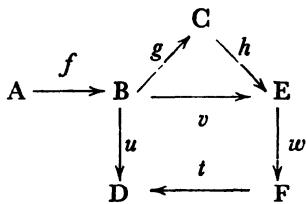
\includegraphics[keepaspectratio]{images/part003_3866b0bf02291d28d06ad2c75d3a73e7be589c55410c746bfd40818492cdc992.jpg}}

in which the letter attached to an arrow denotes a mapping of the set at the tail of the arrow into the set at its head.

The relation of equality ``f=g'' between mappings of E into F is equivalent to the relation ``for all \(x \in E, f(x) = g(x)\) ''.

\begin{enumerate}
\def\labelenumi{\arabic{enumi}.}
\setcounter{enumi}{2}
\tightlist
\item
  A function, defined on a set E, which takes the same value a for every element x of E, is called a constant function on E; it is determined by the functional relation y = a.
\end{enumerate}

The mapping of E into E which associates with each element x of E this same element is called the identity mapping. It is determined by the functional relation y = x.

If A is any subset of E, the mapping of A into E which associates with each element x of A the same element x considered as an element of E is called the canonical mapping of A into E.

Let \(f\) be a mapping of a set \(\mathbf{E}\) into itself. An element \(x\) of \(\mathbf{E}\) is said to be fixed (or invariant) under \(f\) if \(f(x) = x\) .

An element x of E is said to be fixed (or invariant) under a set of mappings of E into E if it is fixed under each of them.

\begin{enumerate}
\def\labelenumi{\arabic{enumi}.}
\setcounter{enumi}{3}
\tightlist
\item
  Let \(f\) be a mapping of \(\mathbf{E}\) into \(\mathbf{F}\) and let \(\mathbf{X}\) be any subset of \(\mathbf{E}\) . Then the image of \(\mathbf{X}\) under \(f\) is the subset \(\mathbf{Y}\) of \(\mathbf{F}\) consisting of all elements \(y\) which have the property ``there exists \(x \in \mathbf{E}\) such that \(x \in \mathbf{X}\) and \(f(x) = y\)''.
\end{enumerate}

This defines a relation between X and Y which is functional in Y and therefore determines a mapping of \(\mathfrak{P}(\mathbf{E})\) into \(\mathfrak{P}(\mathbf{F})\) . This mapping is called the canonical extension of f to sets of subsets; by abuse of language it, too, is denoted by f, and we write \(\mathbf{Y}=f(\mathbf{X})\) .

For all \(f\) and \(x\) we have

\[
f (\phi) = \phi \quad \text { and } \quad f (\{x \}) = \{f (x) \}.
\]

By abuse of language, the value \(f(x)\) of \(f\) at \(x\) is also called the image of \(x\) under \(f\) .

If y is a generic element of F, the property `` \(y \in f(E)\) '' may be expressed by saying that ``y is of the form \(f(x)\) ''.

By abuse of language, the image \(f(\mathbf{E})\) of \(\mathbf{E}\) under \(f\) is sometimes called the image of \(f\) .

If we have \(f(\mathbf{E}) = \mathbf{F}\) , that is if for all \(y \in \mathbf{F}\) there exists \(x \in \mathbf{E}\) such that \(y = f(x)\) , then \(f\) is said to be a mapping of \(\mathbf{E}\) onto \(\mathbf{F}\) , or a surjective mapping, or a surjection.

Let \(x\) be any element and \(X\) any subset of \(E\) . Instead of saying that \(f(x)\) is the value of \(f\) at \(x\) , and \(f(X)\) the image of \(X\) under \(f\) , it is sometimes said that \(f\) transforms (or maps) \(x\) into \(f(x)\) and \(X\) into \(f(X)\) ; \(f(x)\) and \(f(X)\) are then called the transforms by \(f\) of \(x\) and \(X\) , respectively.

If f is a mapping of E into itself, a subset X of E is said to be stable under f if \(f(\mathbf{X}) \subset \mathbf{X}\) . The subset X is said to be stable under a set of mappings of E into E if X is stable under each of these mappings.

\begin{enumerate}
\def\labelenumi{\arabic{enumi}.}
\setcounter{enumi}{4}
\tightlist
\item
  Let \(f\) be a mapping of \(\mathbf{E}\) into \(\mathbf{F}\) . Then we have the following propositions, in which \(\mathbf{X}\) and \(\mathbf{Y}\) denote arbitrary subsets of \(\mathbf{E}\) :
\end{enumerate}

\begin{enumerate}
\def\labelenumi{(\alph{enumi})}
\item
  The relation \(\mathbf{X} \subset \mathbf{Y}\) implies \(f(\mathbf{X}) \subset f(\mathbf{Y})\) .
\item
  The property \(\mathbf{X} \neq \emptyset\) is equivalent to \(f(\mathbf{X}) \neq \emptyset\) .
\item
  For all \(\tilde{\mathbf{X}}\) , \(\mathbf{Y}\) we have
\end{enumerate}

\begin{enumerate}
\def\labelenumi{(\arabic{enumi})}
\setcounter{enumi}{10}
\tightlist
\item
\end{enumerate}

\[
f (\mathbf {X} \cup \mathbf {Y}) = f (\mathbf {X}) \cup f (\mathbf {Y}),\tag{12}
\]

\[
f (\mathbf {X} \cap \mathbf {Y}) \subset f (\mathbf {X}) \cap f (\mathbf {Y}).
\]

\begin{enumerate}
\def\labelenumi{\arabic{enumi}.}
\setcounter{enumi}{5}
\tightlist
\item
  Let \(f\) be a mapping of \(\mathbf{E}\) into \(\mathbf{F}\) , and let \(\mathbf{Y}\) be any subset of \(\mathbf{F}\) . The inverse image of \(\mathbf{Y}\) under \(f\) is the subset \(\mathbf{X}\) of \(\mathbf{E}\) consisting of all elements \(x\) which have the property \(f(x) \in \mathbf{Y}\) .
\end{enumerate}

This defines a relation between X and Y which is functional in X and therefore determines a mapping of \(\mathfrak{P}(\mathbf{F})\) into \(\mathfrak{P}(\mathbf{E})\) , called the inverse extension of f to sets of subsets, and denoted by \(\overline{f}^{1}\) ; thus we write \(\mathbf{X} = \overline{f}^{1}(\mathbf{Y})\) .

In particular, if \(y\) is an element of \(F\) , then \(f^{1}(\{y\})\) will be the set of all \(x \in E\) such that \(f(x) = y\) . The relations `` \(f(x) = y\) '' and `` \(x \in \overline{f}^{1}(\{y\})\) '' are equivalent. By abuse of language we often write \(\overline{f}^{1}(y)\) in place of \(\overline{f}^{1}(\{y\})\) .

The trace \(X_{A}\) of a subset X of E on a given subset A is the inverse image of X under the canonical mapping of A into E (no. 3).

\begin{enumerate}
\def\labelenumi{\arabic{enumi}.}
\setcounter{enumi}{6}
\tightlist
\item
  Let \(f\) be a mapping of \(\mathbf{E}\) into \(\mathbf{F}\) . Then we have the following propositions, in which \(\mathbf{X}\) and \(\mathbf{Y}\) denote arbitrary subsets of \(\mathbf{F}\) :
\end{enumerate}

\begin{enumerate}
\def\labelenumi{(\alph{enumi})}
\item
  The relation \(\mathbf{X} \subset \mathbf{Y}\) implies \(\overline{f}^1(\mathbf{X}) \subset \overline{f}^1(\mathbf{Y})\) .
\item
  For all X, Y we have
\end{enumerate}

\begin{enumerate}
\def\labelenumi{(\arabic{enumi})}
\setcounter{enumi}{12}
\tightlist
\item
\end{enumerate}

\[
\overline {{f}} ^ {1} (\mathrm{X} \cup \mathrm{Y}) = \overline {{f}} ^ {1} (\mathrm{X}) \cup \overline {{f}} ^ {1} (\mathrm{Y}),\tag{14}
\]

\[
\bar {f} ^ {1} (\mathrm{X} \cap \mathrm{Y}) = \bar {f} ^ {1} (\mathrm{X}) \cap \bar {f} ^ {1} (\mathrm{Y}),\tag{15}
\]

\[
\overline {{f}} ^ {1} (\mathbb {C X}) = \mathbb {C} \overline {{f}} ^ {1} (\mathbf {X}).
\]

Note the difference between formulae (12) and (14); (14) would not be true for all X and Y if we replaced f by an arbitrary mapping of F into E. Again, there is no analogue of (15) for the extension of an arbitrary mapping.

Furthermore, we have \(\overline{f}^{1}(\phi) = \phi\) ; but we can also have \(\overline{f}^{1}(\mathbf{X}) = \phi\) for a non-empty subset \(\mathbf{X}\) of \(\mathbf{F}\) . In order that \(\mathbf{X} \neq \phi\) should imply \(\overline{f}^{1}(\mathbf{X}) \neq \phi\) , it is necessary and sufficient that \(f\) should be a mapping of \(\mathbf{E}\) onto \(\mathbf{F}\) .

\begin{enumerate}
\def\labelenumi{\arabic{enumi}.}
\setcounter{enumi}{7}
\tightlist
\item
  If a mapping \(f\) of \(\mathbf{E}\) into \(\mathbf{F}\) is such that for all \(y \in \mathbf{F}\) there exists at most one \(x \in \mathbf{E}\) such that \(y = f(x)\) (in other words, the set \(\overline{f}^1(y)\) is either empty or consists of a single element), then \(f\) is said to be a one-to-one mapping of \(\mathbf{E}\) into \(\mathbf{F}\) , or an injective mapping, or an injection. We have then, for all subsets \(\mathbf{X}, \mathbf{Y}\) of \(\mathbf{E}\) ,
\end{enumerate}

\[
f (\mathbf {X} \cap \mathbf {Y}) = f (\mathbf {X}) \cap f (\mathbf {Y}).\tag{16}
\]

\begin{enumerate}
\def\labelenumi{\arabic{enumi}.}
\setcounter{enumi}{8}
\tightlist
\item
  If a mapping \(f\) of \(\mathbf{E}\) into \(\mathbf{F}\) is such that for all \(y \in \mathbf{F}\) there exists exactly one \(x \in \mathbf{E}\) such that \(y = f(x)\) (in other words, \(\overline{f}(y)\) consists of a single element), then \(f\) is said to be a one-to-one mapping of \(\mathbf{E}\) onto \(\mathbf{F}\) , or a bijective mapping, or a bijection. Such a mapping may be characterized as being both a mapping of E onto F and a one-to-one mapping of E into F.
\end{enumerate}

If \(f\) is a one-to-one mapping of \(\mathbf{E}\) onto \(\mathbf{F}\) , the relation \(y = f(x)\) is not only functional in \(y\) , but also functional in \(x\) . As a functional relation in \(x\) , it determines a one-to-one mapping of \(\mathbf{F}\) onto \(\mathbf{E}\) , called the inverse of the mapping \(f\) .

Note that the extension of the inverse of f is the same as the inverse of the extension of f.

Let \(g\) be the inverse of \(f\) . Then the relations `` \(y = f(x)\) '' and `` \(x = g(y)\) '' are equivalent. The inverse of \(g\) is \(f\) . If \(f\) is a one-to-one mapping of \(E\) onto \(F\) , we have not only the relation (16) but also, for all subsets \(X\) of \(E\) ,

\[
f (\mathbf {C X}) = \mathbf {C} f (\mathbf {X}).
\]

Moreover, the extension of \(f\) is a one-to-one mapping of \(\mathfrak{P}(\mathbf{E})\) onto \(\mathfrak{P}(\mathbf{F})\) .

A one-to-one mapping of E onto F, together with its inverse mapping, are said to realize a one-to-one correspondence between E and F; alternatively, we say that E and F are put in one-to-one correspondence by these mappings.

A one-to-one mapping of a set E onto itself is called a permutation of E. The identity mapping is a permutation. If a permutation is identical with its inverse, it is said to be involutory; for example, the mapping \(X \rightarrow C X\) of \(\mathfrak{P}(E)\) onto itself is involutory.

\begin{enumerate}
\def\labelenumi{\arabic{enumi}.}
\setcounter{enumi}{9}
\tightlist
\item
  In the following propositions, X denotes an arbitrary subset of E, and Y an arbitrary subset of F :
\end{enumerate}

\begin{enumerate}
\def\labelenumi{(\alph{enumi})}
\tightlist
\item
  If \(f\) is a mapping of \(\mathbf{E}\) into \(\mathbf{F}\) , we have
\end{enumerate}

\begin{enumerate}
\def\labelenumi{(\arabic{enumi})}
\setcounter{enumi}{16}
\tightlist
\item
\end{enumerate}

\[
\overline {{{f}}} ^ {1} (\mathrm{Y}) = \overline {{{f}}} ^ {1} (\mathrm{Y} \cap f (\mathrm{E})),\tag{18}
\]

\[
\mathbf {X} \subset \overline {{f}} ^ {1} (f (\mathbf {X})),\tag{19}
\]

\[
f (\overline {{f}} ^ {1} (\mathbf {Y})) \subset \mathbf {Y}.
\]

\begin{enumerate}
\def\labelenumi{(\alph{enumi})}
\setcounter{enumi}{1}
\item
  The properties ``for all Y, \(f(\bar{f}^{1}(Y)) = Y\) '' and ``f is a mapping of E onto F'' are equivalent.
\item
  The properties ``for all X, \(\overline{f}^{1}(f(X)) = X\) '' and ``f is a one-to-one mapping of E into F'' are equivalent.
\item
  The properties ``for all X and Y,
\end{enumerate}

\[
\bar {f} ^ {1} (f (\mathbf {X})) = \mathbf {X} \quad \text { and } \quad f (\bar {f} ^ {1} (\mathbf {Y})) = \mathbf {Y}"
\]

and ``f is a one-to-one mapping of E onto F'' are equivalent.

\begin{enumerate}
\def\labelenumi{\arabic{enumi}.}
\setcounter{enumi}{10}
\tightlist
\item
  Let E, F, G be three sets, which may or may not be distinct. Let f be a mapping of E into F, and let g be a mapping of F into G. The mapping of E into G whose value at any element x of E is \(g(f(x))\) is called the composition of g and f, and is denoted by \(g \circ f\) , or simply gf if there is no risk of ambiguity.
\end{enumerate}

The equality \(h = g \circ f\) is called a factorization of h.

Note that, if G is distinct from E, we may not speak of the composition of f and g (in that order), and the notation \(f \circ g\) has no meaning. If G is identical with E, then \(f \circ g\) and \(g \circ f\) are not elements of the same set unless F is also identical with E; and even when this is so, it is usually the case that \(f \circ g \neq g \circ f\) . Thus the order of composition of f and g is essential.

Let \(\varphi\) be the composition of \(g\) and \(f\) , let \(\mathbf{X}\) be any subset of \(\mathbf{E}\) , and let \(\mathbf{Z}\) be any subset of \(\mathbf{G}\) . Then we have

\begin{enumerate}
\def\labelenumi{(\arabic{enumi})}
\setcounter{enumi}{19}
\tightlist
\item
\end{enumerate}

\[
\varphi (\mathbf {X}) = g (f (\mathbf {X})),\tag{21}
\]

\[
\overline {{{\varphi}}} ^ {1} (Z) = \overline {{{f}}} ^ {1} (\overline {{{g}}} ^ {1} (Z)).
\]

If \(f\) is a one-to-one mapping of \(\mathbf{E}\) onto \(\mathbf{F}\) , and if \(g\) is a one-to-one mapping of \(\mathbf{F}\) onto \(\mathbf{G}\) , then \(g \circ f\) is a one-to-one mapping of \(\mathbf{E}\) onto \(\mathbf{G}\) .

Let \(h\) be a mapping of \(G\) into a set \(H\) . Then we have

\[
h \circ (g \circ f) = (h \circ g) \circ f;
\]

this mapping of E into H is written \(h \circ g \circ f\) , and is called the composition of the three mappings h, g, f in this order. The composition of more than three mappings is defined similarly.

If \(f\) is a mapping of \(\mathbf{E}\) into itself, the iterates of \(f\) are defined to be the mappings \(f^n\) ( \(n\) an integer \(\geqslant 1\) ) of \(\mathbf{E}\) into itself, defined by induction on \(n\) by means of the relations \(f^1 = f\) , \(f^n = f^{n-1} \circ f\) ; \(f^n\) is called the nth iterate of \(f\) . We have \(f^{m+n} = f^m \circ f^n\) .

\begin{enumerate}
\def\labelenumi{\arabic{enumi}.}
\setcounter{enumi}{11}
\tightlist
\item
  In general, the composition \(\overline{f}^{1} \circ f\) of the inverse extension and the extension of a mapping \(f\) is not the identity mapping of \(\mathfrak{P}(\mathbf{E})\) onto itself. Likewise, \(f \circ \overline{f}^1\) is not usually the identity mapping of \(\mathfrak{P}(\mathbf{E})\) onto itself. These two conditions are satisfied simultaneously only if \(f\) is a bijection of \(\mathbf{E}\) onto \(\mathbf{F}\) .
\end{enumerate}

If \(f\) is a bijection of \(\mathbf{E}\) onto \(\mathbf{F}\) , and if \(g\) denotes the inverse of \(f\) , then the compositions \(g \circ f\) and \(f \circ g\) are respectively the identity mapping of \(\mathbf{E}\) onto \(\mathbf{E}\) and the identity mapping of \(\mathbf{F}\) onto \(\mathbf{F}\) .

Conversely, if \(f\) is a mapping of \(\mathbf{E}\) into \(\mathbf{F}\) , and \(g\) a mapping of \(\mathbf{F}\) into \(\mathbf{E}\) , such that \(g \circ f\) is a permutation of \(\mathbf{E}\) and \(f \circ g\) is a permutation of \(\mathbf{F}\) , then \(f\) is a bijection of \(\mathbf{E}\) onto \(\mathbf{F}\) and \(g\) is a bijection of \(\mathbf{F}\) onto \(\mathbf{E}\) .

If, moreover, \(g \circ f\) is the identity mapping of \(\mathbf{E}\) onto itself, then \(g\) is the inverse of \(f\) .

\begin{enumerate}
\def\labelenumi{\arabic{enumi}.}
\setcounter{enumi}{12}
\item
  Let \(f\) be a mapping of \(\mathbf{E}\) into \(\mathbf{F}\) , and let \(\mathbf{A}\) be any subset of \(\mathbf{E}\) . The mapping \(f_{\mathbf{A}}\) of \(\mathbf{A}\) into \(\mathbf{F}\) whose value at any element \(x\) of \(\mathbf{A}\) is \(f(x)\) is called the restriction of \(f\) to the subset \(\mathbf{A}\) ; it is just the composition of \(f\) and the canonical mapping of \(\mathbf{A}\) into \(\mathbf{E}\) . If two mappings \(f, g\) of \(\mathbf{E}\) into \(\mathbf{F}\) have the same restriction to \(\mathbf{A}\) , they are said to agree (or coincide) on \(\mathbf{A}\) . Conversely, \(f\) is said to be an extension of \(f_{\mathbf{A}}\) to \(\mathbf{E}\) .
\item
  A mapping of a set E onto a set F is also called a parametric representation of F by means of E; E is then called the parameter set of this representation, and the elements of E take the name of parameters.
\end{enumerate}

A family of elements of a set F is by definition a subset of F endowed with a parametric representation; in other words, to be given a family of elements of F is equivalent to being given a mapping of some set E into F. The image of E under this mapping is called the set of elements of the family. Note that two distinct families of elements of F may have the same subset of F as the set of their elements.

With each subset A of a set F we may always associate a family of elements whose set of elements is A. It is enough to consider the family defined by the canonical mapping of A into F.

A family of elements of F, defined by a mapping \(\iota\to x_{i}\) of a set I into F, is denoted by \((x_{i})_{i\in I}\) , or simply \((x_{i})\) if there is no possible ambiguity about the index set.

If \(J\) is a subset of \(I\) , the family \((x_{t})_{t\in J}\) is called the subfamily corresponding to \(J\) of the family \((x_{t})_{t\in I}\) ; it is defined by the restriction to \(J\) of the mapping \(t\to x_t\) .

\section{PRODUCTS OF SETS}

\begin{enumerate}
\def\labelenumi{\arabic{enumi}.}
\tightlist
\item
  Let E, F be two sets, which may or may not be distinct. The ordered pairs \((x, y)\) , whose first element x is any element of E and whose second element y is any element of F, are the elements of a new set, called the product of E by F, and denoted by \(E \times F\) ; E and F are called the factors of \(E \times F\) . Two ordered pairs are considered to be identical only if they have the same first element and the same second element; in other words, the relation `` \((x, y) = (x', y')\) '' is equivalent to the relation `` \(x = x'\) and \(y = y''\) ''. If z is any element of \(E \times F\) , the relation ``x is the first element of the ordered pair \(z''\) is a functional relation in x; it determines a mapping of \(E \times F\) onto E, which is called the first coordinate function, or the first projection, and is denoted by \(pr_{1}\) . Instead of saying ``x is the first element of the ordered pair \(z''\) , we also say ``x is the first coordinate (or projection) of \(z''\) or '' \(x = \mathrm{pr}_1z''\) . Similarly we define the second coordinate function, or second projection, which is a mapping of \(E \times F\) onto \(F\) , denoted by \(\mathrm{pr}_2\) .
\end{enumerate}

The relation `` \(x = \text{pr}_1 z\) and \(y = \text{pr}_2 z\) '' is equivalent to `` \(z = (x, y)\) ''.

The extension of the function \(pr_{1}\) to sets of subsets is denoted by the same symbol, in accordance with the general conventions, and is again called the first projection (here we do not use the term ``coordinate''); similarly for the extension of the second projection.

\begin{enumerate}
\def\labelenumi{\arabic{enumi}.}
\setcounter{enumi}{1}
\tightlist
\item
  A relation R between a generic element x of E and a generic element y of F is a property of the pair \((x, y)\) , and consequently defines a subset of the product \(E \times F\) , called the graph of R. Conversely, every subset A of \(E \times F\) is the graph of the relation \((x, y) \in A\) between x and y.
\end{enumerate}

Let A be a subset of E and let B be a subset of F. We denote by \(A \times B\) the subset of \(E \times F\) defined by the relation `` \(x \in A\) and \(y \in B\) '' between x and y.

\begin{enumerate}
\def\labelenumi{\arabic{enumi}.}
\setcounter{enumi}{2}
\tightlist
\item
  In the following propositions, X and X' denote arbitrary subsets of E, Y and Y' arbitrary subsets of F, and Z an arbitrary subset of E × F.
\end{enumerate}

\begin{enumerate}
\def\labelenumi{(\alph{enumi})}
\item
  The relation ``X × Y = φ'' is equivalent to ``X = φ or Y = φ''.
\item
  If \(X \times Y \neq \emptyset\) , the relation `` \(X \times Y \subset X' \times Y''\) '' is equivalent to `` \(X \subset X'\) and \(Y \subset Y''\) ''.
\item
  For all \(\mathbf{X},\mathbf{X}^{\prime},\mathbf{Y}\) we have
\end{enumerate}

\[
(\mathbf {X} \times \mathbf {Y}) \cup (\mathbf {X} ^ {\prime} \times \mathbf {Y}) = (\mathbf {X} \cup \mathbf {X} ^ {\prime}) \times \mathbf {Y}.\tag{22}
\]

\begin{enumerate}
\def\labelenumi{(\alph{enumi})}
\setcounter{enumi}{3}
\tightlist
\item
  For all \(\mathbf{X},\mathbf{X}^{\prime},\mathbf{Y},\mathbf{Y}^{\prime}\) we have
\end{enumerate}

\[
(\mathbf {X} \times \mathbf {Y}) \cap (\mathbf {X} ^ {\prime} \times \mathbf {Y} ^ {\prime}) = (\mathbf {X} \cap \mathbf {X} ^ {\prime}) \times (\mathbf {Y} \cap \mathbf {Y} ^ {\prime}).
\]

\begin{enumerate}
\def\labelenumi{(\alph{enumi})}
\setcounter{enumi}{4}
\tightlist
\item
  For all X, Y we have
\end{enumerate}

\[
\mathrm{pr} _ {1} ^ {- 1} (\mathbf {X}) = \mathbf {X} \times \mathbf {F}, \quad \mathrm{pr} _ {2} ^ {- 1} (\mathbf {Y}) = \mathbf {E} \times \mathbf {Y}.\tag{24}
\]

\begin{enumerate}
\def\labelenumi{(\alph{enumi})}
\setcounter{enumi}{5}
\tightlist
\item
  If \(\mathbf{Y} \neq \emptyset\) , then for all \(\mathbf{X}\) we have
\end{enumerate}

\[
\operatorname{pr} _ {1} (\mathbf {X} \times \mathbf {Y}) = \mathbf {X}.\tag{25}
\]

\begin{enumerate}
\def\labelenumi{(\alph{enumi})}
\setcounter{enumi}{6}
\tightlist
\item
  For all Z we have
\end{enumerate}

\[
Z \subset \operatorname{pr} _ {1} (Z) \times \operatorname{pr} _ {2} (Z).\tag{26}
\]

\begin{enumerate}
\def\labelenumi{(\alph{enumi})}
\setcounter{enumi}{7}
\tightlist
\item
  Let \(a\) be an element of \(\mathbf{E}\) . Then the mapping \((a, y) \to y\) of the set \(\{a\} \times \mathbf{F}\) onto \(\mathbf{F}\) (i.e., the restriction of \(\mathbf{pr}_2\) to the subset \(\{a\} \times \mathbf{F}\) ) is one-to-one.
\end{enumerate}

\begin{enumerate}
\def\labelenumi{\arabic{enumi}.}
\setcounter{enumi}{3}
\item
  The mapping

\[
(x, y) \rightarrow (y, x)\tag{27}
\]

is a one-to-one mapping of \(E \times F\) onto \(F \times E\) , and is called canonical. When E and F are the same set, the mapping (27) is called the canonical symmetry; it is then involutory. The elements \((x, y)\) of \(E \times E\) which are fixed under this symmetry are those which have the property x = y; the set \(\Delta\) of these elements is called the diagonal of \(E \times E\) . The mapping \(x \to (x, x)\) is a bijection of E onto \(\Delta\) , called the diagonal mapping of E into \(E \times E\) .

If Z is any subset of \(E \times F\) , the image of Z under the canonical mapping of \(E \times F\) onto \(F \times E\) is denoted by \(\overline{Z}^{1}\) . If X is any subset of E and Y any subset of F, then

\[
\overline{\mathbf {X} \times \mathbf {Y}}^{1} = \mathbf {Y} \times \mathbf {X}.
\]

If a relation R between x and y, considered as a property of the ordered pair \((x, y)\) , defines a subset A of \(E \times F\) , then the same relation, considered as a property of the pair \((y, x)\) , defines the subset \(\overline{A}^{1}\) of \(F \times E\) . R is equivalent to each of the relations \((x, y) \in A\) , \((y, x) \in \overline{A}^{1}\) . If E and F are the same set, the relation R and the corresponding subset A are said to be symmetric when \(A = \overline{A}^{1}\) . The diagonal \(\Delta\) (defined by the relation of equality) is symmetric. If Z is any subset of \(E \times E\) , then \(Z \cup \overline{Z}^{1}\) and \(Z \cap \overline{Z}^{1}\) are symmetric.

\end{enumerate}

\begin{enumerate}
\def\labelenumi{\arabic{enumi}.}
\setcounter{enumi}{4}
\tightlist
\item
  Let A be a subset of a set E, and let f be a mapping of A into a set F. The relation `` \(x \in A\) and \(y = f(x)\) '' between a generic element x of E and a generic element y of F defines a subset of \(E \times F\) called the graph of the function f.~If B is a subset of E which contains A, and if g is an extension (§ 2, no. 13) of f to B, then the graph of f is contained in the graph of g.
\end{enumerate}

Conversely, let C be a subset of \(\mathbf{E} \times \mathbf{F}\) such that, for each \(x \in \mathbf{E}\) , there exists at most one \(y \in \mathbf{F}\) such that \((x, y) \in \mathbf{C}\) . Then the relation \((x, y) \in \mathbf{C}\) between a generic element \(x\) of the set \(\operatorname{pr}_1(\mathbf{C})\) and a generic element \(y\) of \(\mathbf{F}\) is a functional relation in \(y\) and determines a mapping of \(\operatorname{pr}_1(\mathbf{C})\) into \(\mathbf{F}\) whose graph is \(\mathbf{C}\) .

The set of subsets C of \(E \times F\) which have the property ``for all \(x \in E\) there is at most one \(y \in F\) such that \((x, y) \in C\) '' (a set which is a subset of \(\mathfrak{P}(\mathbf{E} \times \mathbf{F})\) ) can therefore be put into one-to-one correspondence with the set of mappings of subsets of E into F.

Let \(f\) be an injective mapping of \(\mathbf{E}\) into \(\mathbf{F}\) , and let \(g\) be the inverse of \(f\) considered as a bijection of \(\mathbf{E}\) onto \(f(\mathbf{E})\) . If \(\mathbf{C}\) is the graph of \(f\) , then the graph of \(g\) is \(\overline{\mathbf{C}}^1\) .

\begin{enumerate}
\def\labelenumi{\arabic{enumi}.}
\setcounter{enumi}{5}
\tightlist
\item
  If \(f\) is a mapping of \(\mathbf{E}\) into \(\mathbf{F}\) , and \(\mathbf{C}\) is its graph in \(\mathbf{E} \times \mathbf{F}\) , the relation `` \(y = f(x)\) '' is equivalent to `` \((x, y) \in \mathbf{C}\) ''. The relation `` \(y \in f(\mathbf{X})\) '' is equivalent to ``there exists \(x\) such that \(x \in \mathbf{X}\) and \((x, y) \in \mathbf{C}\) ''.
\end{enumerate}

Now let K be any subset of E × F, and let X be any subset of E. Let K(X) denote the subset of F consisting of all elements y which satisfy the relation ``there exists x such that \(x \in X\) and \((x, y) \in K\) ''; this relation is thus equivalent to `` \(y \in K(X)\) ''. The mapping \(X \to K(X)\) of \(\mathfrak{P}(E)\) into \(\mathfrak{P}(F)\) is said to be defined by the subset K of E × F. Note that K(X) is the second projection of the set \(K \cap (X \times F)\) . If K is the graph of a mapping f of E into F, then the mapping \(X \to K(X)\) is the canonical extension of f to sets of subsets.

\begin{enumerate}
\def\labelenumi{\arabic{enumi}.}
\setcounter{enumi}{6}
\tightlist
\item
  If \(x\) is a generic element of \(\mathbf{E}\) , then \(x \to \mathrm{K}(\{x\})\) is a mapping of \(\mathbf{E}\) into \(\mathfrak{P}(\mathbf{F})\) whose value \(\mathrm{K}(\{x\})\) (denoted also by \(\mathrm{K}(x)\) , by abuse of language) is called the section of \(\mathbf{K}\) at \(x\) . The relation \((x, y) \in \mathbf{K}\) is equivalent to \(y \in \mathrm{K}(x)\) .
\end{enumerate}

Conversely, every mapping \(x \to \Phi(x)\) of \(E\) into \(\mathfrak{P}(F)\) can be obtained in this way; for the relation \(y \in \Phi(x)\) defines a subset \(K\) of \(E \times F\) , and \(\Phi(x)\) is precisely the section of \(K\) at \(x\) . The set \(\mathfrak{P}(E \times F)\) and the set of mappings of \(E\) into \(\mathfrak{P}(F)\) are thus in one-to-one correspondence.

\begin{enumerate}
\def\labelenumi{\arabic{enumi}.}
\setcounter{enumi}{7}
\tightlist
\item
  Every mapping \(\mathbf{X} \to \mathbf{K}(\mathbf{X})\) defined by a subset \(\mathbf{K}\) of \(\mathbf{E} \times \mathbf{F}\) has the following properties, which generalize those of the canonical extension of a mapping of \(\mathbf{E}\) into \(\mathbf{F}\) (§2, nos. 4 and 5):
\end{enumerate}

\begin{enumerate}
\def\labelenumi{(\alph{enumi})}
\item
  \(\mathbf{K}(\phi)=\phi.\)
\item
  ``X ⊂ Y'' implies ``K(X) ⊂ K(Y)''.
\item
  For all X, Y we have
\end{enumerate}

\begin{enumerate}
\def\labelenumi{(\arabic{enumi})}
\setcounter{enumi}{27}
\tightlist
\item
\end{enumerate}

\[
\mathbf {K} (\mathbf {X} \cup \mathbf {Y}) = \mathbf {K} (\mathbf {X}) \cup \mathbf {K} (\mathbf {Y}),\tag{29}
\]

\[
\mathbf {K} (\mathbf {X} \cap \mathbf {Y}) \subset \mathbf {K} (\mathbf {X}) \cap \mathbf {K} (\mathbf {Y}).
\]

If K and \(K'\) are two subsets of \(E \times F\) such that \(K \subset K'\) , then we have \(\mathrm{K}(\mathrm{X}) \subset \mathrm{K}'(\mathrm{X})\) for all \(X \subset E\) ; in particular, \(\mathrm{K}(x) \subset \mathrm{K}'(x)\) for all \(x \in E\) . Conversely, if \(\mathrm{K}(x) \subset \mathrm{K}'(x)\) for all \(x \in E\) , then \(K \subset K'\) .

\begin{enumerate}
\def\labelenumi{\arabic{enumi}.}
\setcounter{enumi}{8}
\tightlist
\item
  A relation between a generic element of E and a generic element of F defines a subset K of \(E \times F\) and a subset \(\overline{K}\) of \(F \times E\) , and hence a mapping \(X \to K(X)\) of \(\mathfrak{P}(E)\) into \(\mathfrak{P}(F)\) and a mapping \(Y \to \overline{K}(Y)\) of \(\mathfrak{P}(F)\) into \(\mathfrak{P}(E)\) .
\end{enumerate}

If \(\mathbf{K}\) is the graph of a mapping \(f\) of \(\mathbf{E}\) into \(\mathbf{F}\) , the mapping \(\mathbf{Y} \to \overline{\mathbf{K}}(\mathbf{Y})\) is the inverse extension of \(f\) .

It should be noted that the relations (18) and (19) do not generalize to the mappings \(\mathbf{X} \to \mathbf{K}(\mathbf{X})\) and \(\mathbf{Y} \to \overline{\mathbf{K}}^{1}(\mathbf{Y})\) , when \(\mathbf{K}\) is an arbitrary subset of \(\mathbf{E} \times \mathbf{F}\) .

\begin{enumerate}
\def\labelenumi{\arabic{enumi}.}
\setcounter{enumi}{9}
\tightlist
\item
  Let E, F, G be three sets, which may or may not be distinct, let A be a subset of \(E \times F\) and let B be a subset of \(F \times G\) . Then the elements \((x, z)\) of \(E \times G\) which have the property ``there exists \(y \in F\) such that \((x, y) \in A\) and \((y, z) \in B\) '' form a subset of \(E \times G\) , called the composition of B and A, and denoted by \(B \circ A\) , or simply BA when there is no risk of confusion. Here again, the order of composition is essential. ¶ The mapping \(X \to BA(X)\) of \(\mathfrak{P}(E)\) into \(\mathfrak{P}(G)\) is the composition of \(Y \to B(Y)\) and \(X \to A(X)\) ; in other words, for all \(X \subset E\) we have
\end{enumerate}

\[
\mathbf {B A} (\mathbf {X}) = \mathbf {B} (\mathbf {A} (\mathbf {X})).\tag{30}
\]

Let H be another set, not necessarily distinct from E, F, G, and let C be a subset of \(G \times H\) . Then we have \(\mathbf{C} \circ (\mathbf{B} \circ \mathbf{A}) = (\mathbf{C} \circ \mathbf{B}) \circ \mathbf{A}\) ; this set is also denoted by \(C \circ B \circ A\) (or simply CBA) and is called the composition of C, B, A taken in this order.

Let \(f\) be a mapping of \(\mathbf{E}\) into \(\mathbf{F}\) , and let \(g\) be a mapping of \(\mathbf{F}\) into \(\mathbf{G}\) . If \(\mathbf{A}\) (resp. \(\mathbf{B}\) ) is the graph of \(f\) (resp. \(g\) ), then the composition BA is the graph of the composite mapping \(g \circ f\) .

\begin{enumerate}
\def\labelenumi{\arabic{enumi}.}
\setcounter{enumi}{10}
\tightlist
\item
  We have
\end{enumerate}

\[
\overline{\mathbf {B} \circ \mathbf {A}}^{1} = \overline {\mathbf {A}}^{1} \circ \overline {\mathbf {B}}^{1}.\tag{31}
\]

Let A, A' be two subsets of E × F, and let B, B' be two subsets of F × G. Then the relation

\[
" \mathbf {A} \subset \mathbf {A} ^ {\prime} \text {   and   } \mathbf {B} \subset \mathbf {B} ^ {\prime}" \quad \text { implies } \quad " \mathbf {B} \circ \mathbf {A} \subset \mathbf {B} ^ {\prime} \circ \mathbf {A} ^ {\prime}".
\]

Let A be a subset of \(E \times F\) , \(\Delta\) the diagonal of \(E \times E\) , and \(\Delta'\) the diagonal of \(F \times F\) . Then we have

\[
\mathbf {A} \circ \Delta = \Delta^ {\prime} \circ \mathbf {A} = \mathbf {A}.\tag{32}
\]

\begin{enumerate}
\def\labelenumi{\arabic{enumi}.}
\setcounter{enumi}{11}
\tightlist
\item
  Let E, F, G be three sets, which may or may not be distinct. Their product \(E \times F \times G\) is the set of ordered triples \((x, y, z)\) , where \(x \in E\) , \(y \in F\) , and \(z \in G\) , the relation `` \((x, y, z) = (x', y', z')\) '' being equivalent to `` \(x = x'\) and \(y = y'\) and \(z = z''\) ''. The three mappings \((x, y, z) \to x\) , \((x, y, z) \to y\) , \((x, y, z) \to z\) of \(E \times F \times G\) onto E, F, G respectively are called the first, second, and third coordinate functions (or projections); similarly, for example, the projection with indices 1, 2 is the mapping
\end{enumerate}

\[
(x, y, z) \rightarrow (x, y)
\]

of \(\mathbf{E} \times \mathbf{F} \times \mathbf{G}\) onto \(\mathbf{E} \times \mathbf{F}\) , and is denoted by \(\mathbf{pr}_{1,2}\) .

The definitions and propositions of nos. 2, 3, and 4 generalize easily to the product of three sets.

Furthermore, instead of considering the product \(E \times F \times G\) of three sets, we may equivalently consider the product \((\mathbf{E} \times \mathbf{F}) \times \mathbf{G}\) , obtained by a double application of the operation of forming the product of two sets. In fact, \((x, y, z) \to ((x, y), z)\) is a one-to-one mapping of \(E \times F \times G\) onto \((\mathbf{E} \times \mathbf{F}) \times \mathbf{G}\) , called canonical. Similarly we define one-to-one mappings of \(E \times F \times G\) onto the set \(E \times (F \times G)\) , and onto all the sets obtained from \(E \times F \times G\) , \((\mathbf{E} \times \mathbf{F}) \times \mathbf{G}\) , and \(E \times (F \times G)\) by permuting the three letters E, F, G.

There are analogous definitions and properties for the product of more than three sets.

\begin{enumerate}
\def\labelenumi{\arabic{enumi}.}
\setcounter{enumi}{12}
\tightlist
\item
  If a function \(f\) , which takes its values in any set \(\mathbf{E}'\) , is defined on a product of three sets \(\mathbf{E}\) , \(\mathbf{F}\) , \(\mathbf{G}\) , it is said to be a function of three variables, each of which runs through one of the sets \(\mathbf{E}\) , \(\mathbf{F}\) , \(\mathbf{G}\) . The value of \(f\) at the element \((x, y, z)\) of \(\mathbf{E} \times \mathbf{F} \times \mathbf{G}\) is denoted by \(f(x, y, z)\) .
\end{enumerate}

Let \(a\) be any element of \(\mathbf{E}\) . Then \((y, z) \to f(a, y, z)\) is a mapping of \(\mathbf{F} \times \mathbf{G}\) into \(\mathbf{E}'\) , called a partial mapping (or function) determined by \(f\) corresponding to the value \(a\) of \(x\) ; it is also the composition of \(f\) and the mapping \((y, z) \to (a, y, z)\) of \(\mathbf{F} \times \mathbf{G}\) into \(\mathbf{E} \times \mathbf{F} \times \mathbf{G}\) .

Likewise, if \(b\) is an element of \(\mathbf{F}\) , then \(z \to f(a, b, z)\) is a mapping of \(\mathbf{G}\) into \(\mathbf{E}'\) , called the partial mapping determined by \(f\) corresponding to the values \(a, b\) of \(x, y\) .

Inversely, let g be a mapping of E into \(E'\) . Then \((x, y, z) \to g(x)\) is a mapping h of \(E \times F \times G\) into \(E'\) such that every partial mapping of E into \(E'\) determined by h, corresponding to any values of y and z, is identical with g. This fact is often expressed by saying that a function of an argument x can always be envisaged as a function of all the arguments which need to be considered at a given moment and which will, of course, include x.

\begin{enumerate}
\def\labelenumi{\arabic{enumi}.}
\setcounter{enumi}{13}
\tightlist
\item
  Let \(f, g, h\) be three mappings of \(\mathbf{E}\) into \(\mathbf{E}'\) , \(\mathbf{F}\) into \(\mathbf{F}'\) , \(\mathbf{G}\) into \(\mathbf{G}'\) , respectively. The mapping \((x, y, z) \to (f(x), g(y), h(z))\) of \(\mathbf{E} \times \mathbf{F} \times \mathbf{G}\) into \(\mathbf{E}' \times \mathbf{F}' \times \mathbf{G}'\) is denoted by \((f, g, h)\) or \(f \times g \times h\) and is called the extension of \(f, g, h\) to products. If all three of \(f, g, h\) are injective (resp. surjective, bijective), then \(f \times g \times h\) is injective (resp. surjective, bijective).
\end{enumerate}

In this and the previous subsection we have considered only the case of three sets merely to fix the ideas; analogous considerations hold for any finite number of sets.

\section{UNION, INTERSECTION, PRODUCT OF A FAMILY OF SETS}

\begin{enumerate}
\def\labelenumi{\arabic{enumi}.}
\tightlist
\item
  In this section we consider a family \((\mathbf{X}_{i})_{i\in\mathbf{I}}\) of subsets of a set E, in which the index set I is arbitrary; the set of subsets of E belonging to the family will be denoted by \(\mathfrak{F}\) (which is therefore a subset of \(\mathfrak{P}(\mathbf{E})\) ).
\end{enumerate}

If I is finite, the consideration of the family \((\mathbf{X}_{t})\) reduces to that of several subsets of E, which may or may not be distinct, and in number equal to the number of elements of I. For example, any three subsets \(X_{1}, X_{2}, X_{3}\) of E form a family of subsets of E, the index set here consisting of the numbers 1, 2, 3.

\begin{enumerate}
\def\labelenumi{\arabic{enumi}.}
\setcounter{enumi}{1}
\tightlist
\item
  Let \(J\) be any subset of \(I\) , and consider the set of all elements \(x\) which have the property ``there exists \(\iota \in J\) such that \(x \in X_\iota\)''. This set is called the union of the family of sets \((X_\iota)_{\iota \in J}\) , and is denoted by \(\bigcup_{\iota\in J} X_\iota\) .
\end{enumerate}

We may also formulate this definition as follows: to the mapping \(\iota \to \mathbf{X}_{\iota}\) of \(\mathbf{I}\) into \(\mathfrak{P}(\mathbf{E})\) there corresponds a well-defined subset \(\mathbf{C}\) of \(\mathbf{I} \times \mathbf{E}\) such that \(\mathbf{X}_{\iota} = \mathbf{C}(\iota)\) ( \(\S 3\) , no. 7), and we have \(\bigcup_{\iota \in J} \mathbf{X}_{\iota} = \mathbf{C}(\mathbf{J})\) .

In particular,

\[
\bigcup_ {t \in \varnothing} \mathrm{X} _ {t} = \mathrm{C} (\varnothing) = \varnothing .\tag{33}
\]

When \(J = I\) , we often write \(\bigcup_{i} X_i\) , or simply \(\bigcup X_i\) , in place of \(\bigcup_{i \in I} X_i\) .

The union \(\bigcup_{i} X_{i}\) depends only on the set \(\mathfrak{F}\) ; in other words, it is the same for two families corresponding to the same subset \(\mathfrak{F}\) of \(\mathfrak{P}(E)\) . In particular, it is equal to the union of the family defined by the canonical mapping of \(\mathfrak{F}\) into \(\mathfrak{P}(E)\) , and we may therefore write \(\bigcup_{X \in \mathfrak{F}} X\) , which is also called the union of the sets belonging to \(\mathfrak{F}\) .

When \(\mathbf{I}\) is a set whose elements are explicitly designated, for example the numbers 1, 2, 3, we have

\[
\bigcup_ {i \in I} X _ {i} = X _ {1} \cup X _ {2} \cup X _ {3},
\]

which justifies the name ``union'' given in the general case to the set \(\bigcup_{i}X_{i}\) .

\begin{enumerate}
\def\labelenumi{\arabic{enumi}.}
\setcounter{enumi}{2}
\tightlist
\item
  For any \(J \subset I\) we have
\end{enumerate}

\[
\bigcup_ {i \in J} X _ {i} \subset \bigcup_ {i \in I} X _ {i}.
\]

In particular, for all \(x \in I\) , we have

\[
\mathrm{X} _ {x} \subset \bigcup_ {i \in I} \mathrm{X} _ {i}.
\]

Conversely, if Y is a subset of E such that \(X_{i} \subset Y\) for all \(i \in I\) , then

\[
\bigcup_ {i} \mathrm{X} _ {i} \subset \mathrm{Y}.
\]

More generally, if \((\mathbf{Y}_{i})\) is another family of subsets of E, indexed by the same set I, and if \(X_{i} \subset Y_{i}\) for all \(i \in I\) , then

\[
\bigcup_ {i} X _ {i} \subset \bigcup_ {i} Y _ {i}.
\]

Let F be another set, and let \(\mathbf{X} \to \mathbf{K}(\mathbf{X})\) be the mapping of \(\mathfrak{P}(\mathbf{E})\) into \(\mathfrak{P}(\mathbf{F})\) defined by a subset K of \(E \times F\) . Then we have

\[
\mathrm{K} \left(\bigcup_ {i \in J} \mathrm{X} _ {i}\right) = \bigcup_ {i \in J} \mathrm{K} (\mathrm{X} _ {i}).\tag{34}
\]

Now let \(\mathbf{L}\) be another index set, and \((J_{\lambda})_{\lambda \in \mathbf{L}}\) a family of subsets of \(\mathbf{I}\) . Then

\[
\bigcup_ {\iota \in \bigcup_ {\lambda \in L} J _ {\lambda}} X _ {\iota} = \bigcup_ {\lambda \in L} \left(\bigcup_ {\iota \in J _ {\lambda}} X _ {\iota}\right).\tag{35}
\]

This is the general associativity formula for unions. When I and L are sets whose elements are explicitly designated, the relations we obtain have already been given (see § 1, no. 14). If L alone satisfies this condition and consists, say, of the numbers 1, 2, we have

\[
\bigcup_ {i \in J _ {1} \cup J _ {2}} X _ {i} = \left(\bigcup_ {i \in J _ {1}} X _ {i}\right) \cup \left(\bigcup_ {i \in J _ {2}} X _ {i}\right).\tag{36}
\]

Let \((\mathbf{X}_i)_{i\in I}\) and \((\mathbf{Y}_x)_{x\in K}\) be any two families of subsets of E. Then we have

\[
\left(\bigcup_ {i \in I} X _ {i}\right) \cap \left(\bigcup_ {x \in K} Y _ {x}\right) = \bigcup_ {(i, x) \in I \times K} (X _ {i} \cap Y _ {x}),\tag{37}
\]

the distributivity formula, which includes the second formula of (10) as a particular case.

If \((\mathbf{X}_t)_{i\in \mathbf{I}}\) is a family of subsets of \(\mathbf{E}\) , and if \((\mathbf{Y}_{\mathbf{x}})_{\mathbf{x}\in \mathbf{K}}\) is a family of subsets of \(\mathbf{F}\) , then

\[
\left(\bigcup_ {i \in I} X _ {i}\right) \times \left(\bigcup_ {x \in K} Y _ {x}\right) = \bigcup_ {(i, x) \in I \times K} (X _ {i} \times Y _ {x}).\tag{38}
\]

\begin{enumerate}
\def\labelenumi{\arabic{enumi}.}
\setcounter{enumi}{3}
\tightlist
\item
  A family \((\mathbf{X}_i)_{i\in I}\) of subsets of \(E\) is a covering of a subset \(A\) of \(E\) , or covers \(A\) , if
\end{enumerate}

\[
\mathrm{A} \subset \bigcup_ {i \in \mathrm{I}} \mathrm{X} _ {i}.
\]

In particular, if \((\mathbf{X}_{t})\) is a covering of E, we have

\[
\bigcup_ {i \in I} X _ {i} = E.
\]

A partition of \(\mathbf{E}\) is a covering \((\mathbf{X}_t)\) of \(\mathbf{E}\) such that

\begin{enumerate}
\def\labelenumi{(\alph{enumi})}
\item
  \(\mathbf{X}_{\iota} \neq \varnothing\) for all \(\iota \in \mathbf{I}\) ;
\item
  \(X_{t} \cap X_{x} = \varnothing\) for each pair of different indices t, x in I. (This second condition may be expressed by saying that the \(X_{t}\) are pairwise disjoint.)
\end{enumerate}

These conditions imply that \(\iota \to X_{\iota}\) is a bijection of I onto the set \(\mathfrak{F}\) of subsets of the partition. Hence, if \(\mathfrak{F}\) is given, the family is determined to within a one-to-one correspondence of index sets. In particular, a partition may be considered indifferently as a set of subsets or as a family of subsets.

\begin{enumerate}
\def\labelenumi{\arabic{enumi}.}
\setcounter{enumi}{4}
\tightlist
\item
  Let \((\mathbf{X}_t)_{i \in I}\) be any family of non-empty subsets of a set \(E\) . In the product \(I \times E\) , let \(\mathbf{X}_t'\) denote the subset \(\{\iota\} \times \mathbf{X}_t\) for each \(\iota \in I\) . The set
\end{enumerate}

\[
S = \bigcup_ {i \in I} X _ {i} ^ {\prime}
\]

is called the sum of the family \((\mathbf{X}_i)_{i\in I}\) . It is clear that the family \((\mathbf{X}_i')_{i\in I}\) is a partition of \(S\) and that for each \(i\in I\) the mapping \(x_i\to (i,x_i)\) is a bijection of \(\mathbf{X}_i\) onto \(\mathbf{X}_i'\) . By abuse of language, any set in one-to-one correspondence with \(S\) is often called the sum of the family \((\mathbf{X}_i)_{i\in I}\) , and the \(\mathbf{X}_i\) are usually identified with the subsets of this set to which they correspond.

The sum of two non-empty sets E and F is often said to be obtained by adjoining the set F to E.

\begin{enumerate}
\def\labelenumi{\arabic{enumi}.}
\setcounter{enumi}{5}
\tightlist
\item
  With the notation of no. 2, the set of elements x of E which have the property ``for all \(\iota\in J\) , \(x\in X_{\iota}\) '' is called the intersection of the family of sets \((\mathbf{X}_i)_{i \in J}\) , and is denoted by \(\bigcap_{i \in J} \mathbf{X}_i\) ; when \(J = I\) , we often write \(\bigcap_{i} \mathbf{X}_i\) , or simply \(\bigcap \mathbf{X}_i\) , instead of \(\bigcap_{i \in I} \mathbf{X}_i\) .
\end{enumerate}

We have

\[
\mathbb {C} \left(\bigcup_ {i \in J} X _ {i}\right) = \bigcap_ {i \in J} \left(\mathbb {C} X _ {i}\right).\tag{39}
\]

In particular, if \(\mathrm{J} = \emptyset\) ,

\[
\bigcap_ {i \in \emptyset} X _ {i} = E.\tag{40}
\]

The intersection \(\bigcap_{i} X_i\) depends only on the set \(\mathfrak{F}\) , and may be written \(\bigcap_{X \in \mathfrak{F}} X\) . For example, if \(I\) consists of the numbers 1, 2, 3, we have

\[
\bigcap_ {i} \mathrm{X} _ {i} = \mathrm{X} _ {1} \cap \mathrm{X} _ {2} \cap \mathrm{X} _ {3}.
\]

\begin{enumerate}
\def\labelenumi{\arabic{enumi}.}
\setcounter{enumi}{6}
\tightlist
\item
  Formula (39) allows us to generalize the duality rule. If a subset A of E is obtained from other subsets X, Y, Z and families \((\mathbf{X}_{t}), (\mathbf{Y}_{x}), (\mathbf{Z}_{\lambda})\) of subsets of E by applying (in any order) only the operations \(\mathbb C, \cup, \cap, \bigcup, \bigcap\), then we shall obtain the complement \(\mathbb C A\) by replacing the subsets X, Y, Z, \(X_{t}, Y_{x}, Z_{\lambda}\) by their complements, and the operations \(\cup, \cap, \bigcup, \bigcap\) by \(\cap, \cup, \bigcap, \bigcup\), respectively, the order of operations being preserved; of course, the operations of intersection and union are not to be altered where they apply to index sets written under the signs \(\bigcup\) and \(\bigcap\).
\end{enumerate}

As in §1, no. 15, we define the dual of a relation \(\mathbf{A} = \mathbf{B}\) or \(\mathbf{A} \subset \mathbf{B}\) where \(\mathbf{A}\) and \(\mathbf{B}\) are subsets of \(\mathbf{E}\) of the above form.

\begin{enumerate}
\def\labelenumi{\arabic{enumi}.}
\setcounter{enumi}{7}
\tightlist
\item
  For all \(J \subset I\) we have
\end{enumerate}

\[
\bigcap_ {i \in I} X _ {i} \subset \bigcap_ {i \in J} X _ {i}.
\]

In particular, for all \(x \in I\) we have

\[
\bigcap_ {i} \mathrm{X} _ {i} \subset \mathrm{X} _ {x}.
\]

Conversely, if \(\mathbf{Y} \subset \mathbf{X}_i\) for all \(\iota \in I\) , then

\[
\mathrm{Y} \subset \bigcap_ {i} \mathrm{X} _ {i}.
\]

More generally, if \((\mathbf{Y}_{t})\) is another family of subsets of E, indexed by the same set I, and if \(X_{t} \subset Y_{t}\) for all \(t \in I\) , then

\[
\bigcap_ {i} X _ {i} \subset \bigcap_ {i} Y _ {i}.
\]

The union of the sets \(X_{t}\) is the intersection of all sets Y such that \(X_{t} \subset Y\) for all \(t \in I\) . The intersection of the \(X_{t}\) is the union of all Z such that \(Z \subset X_{t}\) for all \(t \in I\) .

The following formulae are the duals of (35) and (37), respectively:

\begin{enumerate}
\def\labelenumi{(\arabic{enumi})}
\setcounter{enumi}{40}
\tightlist
\item
\end{enumerate}

\[
\bigcap_ {i \in \bigcup_ {\lambda \in L} J _ {\lambda}} X _ {i} = \bigcap_ {\lambda \in L} \left(\bigcap_ {i \in J _ {\lambda}} X _ {i}\right) \quad (\text { associativity });\tag{42}
\]

\[
\left(\bigcap_ {t \in I} X _ {t}\right) \cup \left(\bigcap_ {x \in K} Y _ {x}\right) = \bigcap_ {(t, x) \in I \times K} (X _ {t} \cup Y _ {x}) \quad (\text { distributivity }).
\]

If \((\mathbf{X}_i)_{i\in I}\) is a family of subsets of \(\mathbf{E}\) , and \((\mathbf{Y}_x)_{x\in \mathbb{K}}\) a family of subset of \(\mathbf{F}\) , then

\[
\left(\bigcap_ {i \in I} X _ {i}\right) \times \left(\bigcap_ {x \in K} Y _ {x}\right) = \bigcap_ {(i, x) \in I \times K} (X _ {i} \times Y _ {x}).\tag{43}
\]

Moreover, if \((\mathbf{X}_{t})\) and \((\mathbf{Y}_{t})\) are families of subsets of E and F, respectively, indexed by the same set I, then

\[
\left(\bigcap_ {i \in I} X _ {i}\right) \times \left(\bigcap_ {i \in I} Y _ {i}\right) = \bigcap_ {i \in I} (X _ {i} \times Y _ {i}).\tag{44}
\]

The formula (34) has no dual; in general all we can say is

\[
\mathrm{K} \left(\bigcap_ {i \in J} X _ {i}\right) \subset \bigcap_ {i \in J} \mathrm{K} (X _ {i}).\tag{45}
\]

We have equality in (45) for all families \((\mathbf{X}_{t})\) only if \(\mathbf{X} \to \mathbf{K}(\mathbf{X})\) is the inverse extension of a mapping of a subset of F into E. Consequently, if f is a mapping of F into E, we have (generalizing (14))

\[
\bar {f} ^ {1} \left(\bigcap_ {i \in J} X _ {i}\right) = \bigcap_ {i \in J} \bar {f} ^ {1} (X _ {i}).\tag{46}
\]

\begin{enumerate}
\def\labelenumi{\arabic{enumi}.}
\setcounter{enumi}{8}
\tightlist
\item
  Let E be any set and let I be any index set. The set of all families \((x_{i})_{i\in I}\) of elements of E, indexed by I, is denoted by \(E^{I}\) , and the operation of passing from E to \(E^{I}\) is called exponentiation. \(E^{I}\) is thus in one-to-one correspondence with the set of all mappings of I into E (which for this reason is often denoted by \(E^{I}\) , by abuse of language), as well as with a subset of \(\mathfrak{P}(\mathbf{I} \times \mathbf{E})\) , by considering the graphs of these mappings. The sets \(E^{J}\) corresponding to subsets J of the set I may therefore be considered all as subsets of the same set, which is in one-to-one correspondence with a subset of \(\mathfrak{P}(\mathbf{I} \times \mathbf{E})\) .
\end{enumerate}

Now let \((\mathbf{X}_i)_{i\in I}\) be a family of subsets of E, indexed by the same set I, and let J be any subset of I. The property ``for all \(i\in J\) , \(x_i\in X_i\)'' of the family \((x_i)_{i\in J}\) defines a subset of \(\mathbf{E}^{\mathbf{J}}\) , called the product of the family of sets \((\mathbf{X}_i)_{i\in J}\) , and denoted by \(\prod_{i\in J}\mathbf{X}_i\) (or simply \(\prod_{i}\mathbf{X}_i\) when \(J = I\) ). The \(\mathbf{X}_i\) are called the factors of the product. Note that \(\prod_{i\in \emptyset}\mathbf{X}_i\) is a set consisting of one element (corresponding to the empty subset of \(\mathbf{I}\times \mathbf{E}\) ). If \(\mathbf{X}_i = \mathbf{E}\) for all \(i\in J\) , then we have

\[
\prod_ {i \in J} X _ {i} = E ^ {J}.
\]

If, for example, I consists of the three numbers 1, 2, 3, then \(\prod_{i\in J}X_i\) is in one-to-one correspondence with the set \(X_1\times X_2\times X_3\) . 10. If \(R\{x,y\}\) is a relation between a generic element \(x\) of a set E and a generic element \(y\) of a set F, then the following propositions are equivalent:

``for each x there exists y such that R\{x,y\}''

and

``there exists a mapping f of E into F such that R\{x, f(x)\} for all x''.

The assertion of this equivalence is known as the axiom of choice (or Zermelo's axiom). We shall sometimes indicate whether the proof of a theorem depends on it.

The axiom of choice is equivalent to the following proposition: ``if, for each \(\iota\in I\) , we have \(X_{\iota}\neq\phi\) , then \(\prod_{\iota\in I}X_{\iota}\neq\phi\) ''.

\begin{enumerate}
\def\labelenumi{\arabic{enumi}.}
\setcounter{enumi}{10}
\tightlist
\item
  In this and the following subsection, we shall consider a non-empty product \(\prod A_{i}\) , where \((A_{i})\) is any family of (non-empty) subsets of E.
\end{enumerate}

Let \(J\) be a subset of \(I\) . The mapping \((x_{i})_{i\in I}\to(x_{i})_{i\in J}\) of \(\prod_{i\in I}A_{i}\) onto \(\prod_{i\in J}A_{i}\) is called the projection of \(\prod_{i\in I}A_{i}\) onto \(\prod_{i\in J}A_{i}\) , and is denoted by \(pr_{J}\) . In particular, the mapping \((x_{i})_{i\in I}\to x_{x}\) of \(\prod_{i\in I}A_{i}\) onto \(A_{x}\) is called the coordinate function (or projection) of index \(x\) , and is denoted by \(pr_{x}\) .

If \(z\) is an element of \(\prod_{i} A_{i}\) , we have \(z = (\mathrm{pr}_{i}z)_{i \in I}\) .

Let \(J_1, J_2\) be two sets forming a partition of I. Then \(z \to (\mathrm{pr}_{J_1}z, \mathrm{pr}_{J_2}z)\) is a one-to-one mapping of \(\prod_{i\in I} A_i\) onto \(\prod_{i\in J_1} A_i \times \prod_{i\in J_2} A_i\) .

In general, if \((\mathbf{J}_{\lambda})_{\lambda \in \mathbf{L}}\) is any partition of the set I, the mapping \(z \to (\mathrm{pr}_{\mathbf{J}_{\lambda}} z)_{\lambda \in \mathbf{L}}\) is a bijection (called canonical) of \(\prod_{i \in I} A_i\) onto the product \(\prod_{\lambda \in L} \left( \prod_{i \in J_{\lambda}} A_i \right)\) . This may also be expressed by saying that the product of a family of sets is associative.

\begin{enumerate}
\def\labelenumi{\arabic{enumi}.}
\setcounter{enumi}{11}
\tightlist
\item
  The following propositions generalize those of §3, no. 3; \((\mathbf{X}_t)\) , \((\mathbf{Y}_t)\) denote families of subsets of E such that \(\mathbf{X}_t \subset \mathbf{A}_t\) and \(\mathbf{Y}_t \subset \mathbf{A}_t\) for all \(t \in I\) ; Z denotes any subset of \(\prod A_t\) .
\end{enumerate}

\begin{enumerate}
\def\labelenumi{(\alph{enumi})}
\item
  If \(\prod_{i} X_{i} \neq \emptyset\) , the relation `` \(\prod_{i} X_{i} \subset \prod_{i} Y_{i}\) '' is equivalent to ``for all \(i \in I\) , \(X_{i} \subset Y_{i}\) ''.
\item
  We have \(\operatorname{pr}_{\chi}^{-1}(\mathbf{X}_{\chi}) = \prod_{i} \mathbf{Y}_{i}\) , where \(\mathbf{Y}_{\chi} = \mathbf{X}_{\chi}\) and \(\mathbf{Y}_{i} = \mathbf{A}_{i}\) whenever \(i \neq \chi\) . Hence
\end{enumerate}

\[
\prod_ {i \in I} X _ {i} = \bigcap_ {i \in I} \operatorname{pr}_{i}^{-1}(X _ {i}).\tag{47}
\]

\begin{enumerate}
\def\labelenumi{(\alph{enumi})}
\setcounter{enumi}{2}
\tightlist
\item
  If \(\prod_{i} X_i \neq \emptyset\) , then
\end{enumerate}

\[
\operatorname{pr} _ {x} \left(\prod_ {i} X _ {i}\right) = X _ {x}.\tag{48}
\]

\begin{enumerate}
\def\labelenumi{(\alph{enumi})}
\setcounter{enumi}{3}
\tightlist
\item
  For all Z we have
\end{enumerate}

\[
\mathbf {Z} \subset \prod_ {\iota} \operatorname{pr} _ {\iota} (\mathbf {Z}).\tag{49}
\]

\begin{enumerate}
\def\labelenumi{(\alph{enumi})}
\setcounter{enumi}{4}
\tightlist
\item
  Let \((\mathbf{J}_1, \mathbf{J}_2)\) be a partition of I into two sets, let \((a_t)_{t \in J_1}\) be a family of elements of E, and let \((\mathbf{X}_t)_{t \in J_2}\) be a family of subsets of E, such that \(a_t \in \mathbf{A}_t\) for all \(t \in J_1\) , and \(\mathbf{X}_t \subset \mathbf{A}_t\) for all \(t \in J_2\) . Then the product \(\prod_{i \in I} \mathbf{Y}_t\) , where \(\mathbf{Y}_t = \{a_t\}\) when \(t \in J_1\) , and \(\mathbf{Y}_t = \mathbf{X}_t\) when \(t \in J_2\) , can be put in one-to-one correspondence with \(\prod_{i \in J_2} \mathbf{X}_t\) by projecting onto this latter set.
\end{enumerate}

\begin{enumerate}
\def\labelenumi{\arabic{enumi}.}
\setcounter{enumi}{12}
\tightlist
\item
  Let \((\mathbf{A}_i)_{i\in I}\) be a family of subsets of a set \(F\) , and let \(f\) be a mapping of a set \(E\) into the product \(\prod_{i\in I} A_i\) . If we put \(f_i(x) = \text{pr}_i(f(x))\) , then \(f_i\) is a mapping of \(E\) into \(A_i\) , and \(f\) is the mapping \(x \to (f_i(x))\) . Conversely, if for each index \(i \in I\) , \(f_i\) is a mapping of \(E\) into \(A_i\) , then
\end{enumerate}

\[
x \rightarrow (f _ {i} (x))
\]

is a mapping of E into \(\prod_{i\in I}A_i\) , which is denoted by \((f_i)\) (by abuse of language, because this notation already denotes the family of mappings \(f_i\) ). Thus we define a bijection (called canonical) of the set \(\left(\prod_{i\in I}A_i\right)^E\) onto the set \(\prod_{i\in I}(A_i^E)\) .

\begin{enumerate}
\def\labelenumi{\arabic{enumi}.}
\setcounter{enumi}{13}
\item
  Let E, F, G be three sets. For each mapping f of \(F \times G\) into E and for each \(y \in G\) , let \(f_{y}\) denote the partial mapping \(x \to f(x, y)\) of F into E. Then \(y \to f_{y}\) is a mapping of G into \(E^{F}\) . Conversely, for each mapping g of G into \(E^{F}\) there exists a unique mapping f of \(F \times G\) into E such that \(f_{y} = g(y)\) for all \(y \in G\) . Thus we define a bijection (called canonical) of the set \(E^{F \times G}\) onto the set \((E^{F})^{G}\) .
\item
  Let \((\mathbf{A}_t)_{t \in \mathbf{I}}\) be a family of non-empty subsets of a set \(\mathbf{E}\) . For each \(t \in I\) let \(f_t\) be a mapping of \(\mathbf{A}_t\) into a set \(\mathbf{F}\) such that, for each pair of indices \((t, x)\) , \(f_t\) and \(f_x\) agree on \(\mathbf{A}_t \cap \mathbf{A}_x\) . Then, if
\end{enumerate}

\[
\mathrm{A} = \bigcup_ {i \in \mathrm{I}} \mathrm{A} _ {i},
\]

there exists a unique mapping \(f\) of \(\mathbf{A}\) into \(\mathbf{F}\) such that the restriction of \(f\) to each \(\mathbf{A}_i\) is equal to \(f_i\) . In particular, if \(\mathbf{A}_i \cap \mathbf{A}_x = \emptyset\) whenever \(i \neq x\) , we see that sets \(\mathbf{F}^{\mathbf{A}}\) and \(\prod_{i \in I} \mathbf{F}^{\mathbf{A}_i}\) are in one-to-one correspondence (called canonical).

\section{EQUIVALENCE RELATIONS AND QUOTIENT SETS}

\begin{enumerate}
\def\labelenumi{\arabic{enumi}.}
\tightlist
\item
  Let \((\mathbf{A}_t)_{i \in \mathbf{I}}\) be a partition of a set \(\mathbf{E}\) . The relation \(\mathbf{R}\{x, y\} :\) ``there exists \(i \in \mathbf{I}\) such that \(x \in \mathbf{A}_t\) and \(y \in \mathbf{A}_t\)'' between two generic elements \(x, y\) of \(\mathbf{E}\) satisfies the following conditions:
\end{enumerate}

\begin{enumerate}
\def\labelenumi{(\alph{enumi})}
\item
  \(\mathbf{R}\{x,x\}\) is an identity (reflexivity of \(\mathbf{R}\) ).
\item
  \(\mathbf{R}\{x,y\}\) and \(\mathbf{R}\{y,x\}\) are equivalent (symmetry of \(\mathbf{R}\) ).
\item
  The relation ``R\{x,y\} and R\{y,z\}'' implies R\{x,z\} (transitivity of R).
\end{enumerate}

If C denotes the subset of \(E \times E\) defined by the relation R, the conditions (a), (b), (c) are respectively equivalent to the following conditions: \((a') \Delta \subset C; (b') \overline{C} = C; (c') C \circ C \subset C.\) From \((a')\) and \((c')\) it follows that \(C \circ C = C.\)

\begin{enumerate}
\def\labelenumi{\arabic{enumi}.}
\setcounter{enumi}{1}
\tightlist
\item
  Conversely, let \(R\{x,y\}\) be a reflexive, symmetric, and transitive relation, and let C be its graph in \(E \times E\) . Then the image F of E under the mapping \(x \to C(x)\) of E into \(\mathfrak{P}(E)\) is a partition of E, and the relation ``there exists a subset \(X \in F\) such that \(x \in X\) and \(y \in X\) '' is equivalent to \(R\{x, y\}\) .
\end{enumerate}

Every relation which satisfies conditions (a), (b), and (c) is called an equivalence relation on E. The partition \(\mathfrak{F}\) which it defines, considered as a subset of \(\mathfrak{P}(\mathbf{E})\) , is called the quotient set of E by the relation R, and is denoted by E/R; its elements are called equivalence classes with respect to R. The mapping \(x \to \mathrm{C}(x)\) of E onto E/R, which maps each element \(x\) of E to the equivalence class which contains \(x\) , is called the canonical mapping of E onto E/R.

The relation of equality x = y is an equivalence relation. The canonical mapping of E onto the corresponding quotient set is just \(x \to \{x\}\) , and is bijective.

If R is an equivalence relation, the notation `` \(x \equiv y \pmod{R}\) '' is sometimes used as a synonym for R \(\{x, y\}\) ; it is read `` \(x\) is equivalent to \(y\) modulo R''.

\begin{enumerate}
\def\labelenumi{\arabic{enumi}.}
\setcounter{enumi}{2}
\tightlist
\item
  On a product set \(E \times F\) , the relation `` \(pr_{1}z = pr_{1}z'\) '' between z and \(z'\) is an equivalence relation R, and the quotient set \((\mathbf{E} \times \mathbf{F}) / \mathbf{R}\) can be put in one-to-one correspondence with E (this is the origin of the name quotient set).
\end{enumerate}

More generally, let \(f\) be a mapping of a set \(\mathbf{E}\) into a set \(\mathbf{F}\) . Then the relation '' \(f(x) = f(y)\) '' is an equivalence relation on \(\mathbf{E}\) . If we denote this relation by \(\mathbf{R}\) , the mapping \(z \to \overline{f}^1(z)\) (where \(\overline{f}^1(z)\) is considered as an element of \(\mathbf{E}/\mathbf{R}\) ) is a bijection of \(f(\mathbf{E})\) onto \(\mathbf{E}/\mathbf{R}\) .

It follows that \(f\) may be considered as the composition of the following three mappings, in the given order:

\begin{enumerate}
\def\labelenumi{(\arabic{enumi})}
\item
  the canonical mapping of the subset \(f(\mathbf{E})\) of \(\mathbf{F}\) into the set \(\mathbf{F}\) ;
\item
  the bijective mapping of E/R onto \(f(\mathbf{E})\) , whose inverse has just been defined;
\item
  the canonical mapping of E onto E/R.
\end{enumerate}

This decomposition of a mapping is called its canonical decomposition or canonical factorization.

\begin{enumerate}
\def\labelenumi{\arabic{enumi}.}
\setcounter{enumi}{3}
\item
  Every equivalence relation R on a set E may be defined by means of a mapping as in the previous subsection; for, if C is the graph of R, the relation ``C(x) = C(y)'' is equivalent to R\{x, y\}.
\item
  Let R be an equivalence relation on a set E, and let A be a subset of E. Then the relation \(R\{x, y\}\) between two generic elements x, y of A is an equivalence relation on A, called the relation induced by R on A, and denoted by \(R_{A}\) . Let f be the canonical mapping of E onto E/R and let g be that of A onto \(A/R_{A}\) . By making an element of E/R and an element of \(A/R_{A}\) correspond if they are the images of the same element of E under f and g respectively, we have a one-to-one correspondence between the image \(f(A)\) of A under f and the quotient set \(A/R_{A}\) . If \(\varphi\) denotes the canonical mapping of A into E, this correspondence is realized by the mapping \(z \to f(\varphi(\overline{g}^1(z)))\) and its inverse, both of which are also called canonical.
\item
  A subset \(\mathbf{A}\) of \(\mathbf{E}\) is said to be saturated with respect to the equivalence relation \(\mathbf{R}\) if for each \(x \in \mathbf{A}\) the equivalence class of \(x\) with respect to \(\mathbf{R}\) is contained in \(\mathbf{A}\) . In other words, the saturated sets with respect to \(\mathbf{R}\) are unions of equivalence classes with respect to \(\mathbf{R}\) . If \(f\) is the canonical mapping of \(\mathbf{E}\) onto \(\mathbf{E} / \mathbf{R}\) , then a set is saturated if it is of the form \(\overline{f}^1(\mathbf{X})\) , where \(\mathbf{X} \subset \mathbf{E} / \mathbf{R}\) .
\end{enumerate}

Let A be a subset of E. The intersection of the saturated sets which contain A is \(\overline{f}^{1}(f(A))\) . This set may also be defined as the union of the equivalence classes of the elements of A, and is called the saturation of A (with respect to R).

\begin{enumerate}
\def\labelenumi{\arabic{enumi}.}
\setcounter{enumi}{6}
\tightlist
\item
  Let \(\mathrm{P}\{x, y, z\}\) be a relation in which there appears a generic element \(x\) of \(\mathbf{E}\) . Then \(\mathrm{P}\) is said to be compatible (in \(x\) ) with the equivalence relation \(\mathbf{R}\) if the relation `` \(\mathrm{P}\{x, y, z\}\) and \(x \equiv x' (\text{mod } \mathbf{R})\) '' implies \(\mathrm{P}\{x', y, z\}\) .
\end{enumerate}

Let \(f\) be the canonical mapping of \(\mathbf{E}\) onto \(\mathbf{E} / \mathbf{R}\) , and let \(t\) be a generic element of \(\mathbf{E} / \mathbf{R}\) . The relation ``there exists \(x \in \overline{f}^1(t)\) such that \(\mathrm{P}\{x, y, z\}\)'' is then equivalent to ``for all \(x \in \overline{f}^1(t)\) , \(\mathrm{P}\{x, y, z\}\) ; the latter is a relation between \(t, y, z\) , said to be induced by \(\mathrm{P}\) on passing to the quotient (with respect to \(x\) ). If we denote it by \(\mathrm{P}'\{t, y, z\}\) , then \(\mathrm{P}\{x, y, z\}\) is equivalent to \(\mathrm{P}'\{f(x), y, z\}\) .

There are analogous definitions for a relation involving any number of arguments, and for the case in which the relation is compatible with R in several of its arguments. For example, if A is a subset of E, to say that the relation `` \(x \in A\) '' is compatible (in \(x\) ) with R is equivalent to saying that A is saturated with respect to R. If \(\varphi\) is a mapping of E into a set F, to say that the functional relation `` \(y = \varphi(x)\) '' is compatible (in \(x\) ) with R is to say that \(\varphi\) is constant on each equivalence class with respect to R. Passing to the quotient, R therefore induces a relation between \(y\) and a generic element \(t\) of E/R; this relation is functional in \(y\) and so determines a mapping \(\varphi'\) of E/R into F, satisfying the identity \(\varphi(x) = \varphi'(f(x))\) .

\begin{enumerate}
\def\labelenumi{\arabic{enumi}.}
\setcounter{enumi}{7}
\item
  Let R be an equivalence relation on a set E, let S be an equivalence relation on a set F, and let f be a mapping of E into F. The mapping f is said to be compatible with R and S if the relation \(x \equiv x' \pmod{R}\) implies \(f(x) \equiv f(x') \pmod{S}\) . If g is the canonical mapping of F onto F/S, then the composite function \(g \circ f\) has the same value at all elements of an equivalence class z with respect to R; if we denote this common value by \(h(z)\) , then h is a mapping of E/R into F/S, and is said to be induced by f on passing to the quotients.
\item
  Let R be an equivalence relation on E, and let S be an equivalence relation on E/R. If f is the canonical mapping of E onto E/R, then `` \(f(x) \equiv f(y) \pmod{S}\) '' is an equivalence relation T on E. An equivalence class with respect to T is therefore the union in E of equivalence classes with respect to R which are equivalent to each other with respect to S; and the relation `` \(x \equiv y \pmod{R}\) '' implies `` \(x \equiv y \pmod{T}\) ''. If \(g\) and \(\varphi\) are the canonical mappings of E/R onto (E/R)/S and E onto E/T, respectively, we obtain a one-to-one correspondence (called canonical) between (E/R)/S and E/T by making an element of (E/R)/S and an element of E/T correspond to each other if they are the images of the same element of E under \(g \circ f\) and \(\varphi\) , respectively.
\end{enumerate}

Conversely, let R and T be two equivalence relations on E such that `` \(x \equiv y \pmod{R}\) '' implies `` \(x \equiv y \pmod{T}\) ''. Then T is compatible (in the sense of no. 7) with R, both in \(x\) and in \(y\) ; by passing to the quotient E/R (with respect to \(x\) and \(y\) ), T induces an equivalence relation S on E/R. If \(f\) again denotes the canonical mapping of E onto E/R, the relation `` \(f(x) = f(y) \pmod{S}\) '' is equivalent to `` \(x \equiv y \pmod{T}\) ''. The equivalence relation S is called the quotient of T by R, and is denoted by T/R. From the previous paragraph we see that there exists a one-to-one correspondence (the canonical correspondence) between (E/R)/(T/R) and E/T.

\begin{enumerate}
\def\labelenumi{\arabic{enumi}.}
\setcounter{enumi}{9}
\tightlist
\item
  Now let E, F be any two sets, which may or may not be distinct. Let R\{x, y\} be an equivalence relation on E and let S\{z, t\} be an equivalence relation on F. Then the relation ``R\{x, y\} and S\{z, t\}'' between elements (x, z) and (y, t) of the product set E × F is an equivalence relation on E × F, called the product of R by S, and denoted by R × S. Every equivalence class with respect to R × S is the product of an equivalence class with respect to R and an equivalence class with respect to S. If u denotes a generic element of E/R, and v a generic element of F/S, then (u, v) → u × v is a bijection (called canonical) of (E/R) × (F/S) onto (E × F)/(R × S).
\end{enumerate}

\section{ORDERED SETS}

\begin{enumerate}
\def\labelenumi{\arabic{enumi}.}
\tightlist
\item
  A relation \(\omega\{x, y\}\) between two generic elements \(x, y\) of a set E is said to be an order relation on E, if it satisfies the following two conditions:
\end{enumerate}

\begin{enumerate}
\def\labelenumi{(\alph{enumi})}
\item
  The relation `` \(\omega \{x, y\}\) and \(\omega \{y, z\}\) '' implies \(\omega \{x, z\}\) (transitivity).
\item
  The relation ``ω\{x, y\} and ω\{y, x\}'' is equivalent to ``x = y''. Condition (b) implies that ω is reflexive.
\end{enumerate}

Let C be the subset of \(E \times E\) defined by the relation \(\omega\{x, y\}\) as a property of the pair \((x, y)\) . Then conditions (a) and (b) are respectively equivalent to the following: \((a') \quad C \circ C \subset C\) ; \((b') \quad C \cap \overline{C} = \Delta\) . These imply that \(C \circ C = C\) .

When we consider a particular order relation on a set E, we say that E is ordered by this relation, and that the relation defines an order structure (cf.~§8) (or an ordering) on E.

If \(\omega\{x,y\}\) is an order relation on E, then so is \(\omega\{y,x\}\) . These two order relations, and the orderings they define, are said to be opposites of each other.

Let \(\omega\{x, y\}\) be an order relation on E, and let A be any subset of E. The relation \(\omega\{x, y\}\) between two generic elements \(x, y\) of A is then an order relation on A, and the ordering it defines on A is said to be induced by the ordering defined by \(\omega\{x, y\}\) on E. The given ordering on E is said to be an extension of the induced ordering on A.

A reflexive and transitive relation \(\varpi\{x, y\}\) between two generic elements \(x, y\) of E is called a preorder relation on E. The relation `` \(\varpi\{x, y\}\) and \(\varpi\{y, x\}\) '' is an equivalence relation R on E, and \(\varpi\{x, y\}\) is compatible (in \(x\) and \(y\) ) with this relation. Passing to the quotient (with respect to \(x\) and \(y\) ), \(\varpi\{x, y\}\) induces on the set E/R an order relation, said to be associated with \(\varpi\{x, y\}\) . A set endowed with a preorder relation is called a preordered set.

\begin{enumerate}
\def\labelenumi{\arabic{enumi}.}
\setcounter{enumi}{1}
\tightlist
\item
  The inclusion relation ``Y ⊂ X'' is an order relation on the set of subsets \(\mathfrak{P}(\mathbf{E})\) of any set E.
\end{enumerate}

If E and F are two sets, which may or may not be distinct, the relation ``g extends f'' is an order relation on the set of all mappings of subsets of E into F.

The set N of natural integers (*) is ordered by the relation `` \(x \leqslant y\) ''. 3. By analogy with this last example, when a set E is ordered by a relation \(\omega\{x, y\}\) , it is often convenient to denote the relation \(\omega\{x, y\}\) by \(x \leqslant y\) , or \(y \geqslant x\) ; these relations are read `` \(x\) is less than \(y\) '', or `` \(y\) is greater than \(x\) '' (†). The relations `` \(x < y\) '' and `` \(y > x\) '' (read `` \(x\) is strictly less than \(y\) '', or `` \(y\) is strictly greater than \(x\) '') are by definition equivalent to `` \(x \leqslant y\) and \(x \neq y\) ''.

The relation ``x ≤ y'' is equivalent to ``x \textless{} y or x = y''. The relation ``x ≤ y and y \textless{} z'' implies ``x \textless{} z''; similarly, ``x \textless{} y and y ≤ z'' implies ``x \textless{} z''.

\begin{enumerate}
\def\labelenumi{\arabic{enumi}.}
\setcounter{enumi}{3}
\tightlist
\item
  A subset X of a set E, ordered by a relation `` \(x \leqslant y\) '', is said to be totally ordered by this relation if, for all \(x \in X\) and all \(y \in X\) , we have either \(x \leqslant y\) or \(y \leqslant x\) (or, equivalently, either x \textless{} y or x = y or x \textgreater{} y, these three relations being mutually exclusive).
\end{enumerate}

The empty subset of an ordered set is always totally ordered. It may happen that the whole set E is totally ordered, as is the case for the set N and the relation \(x \leqslant y\) .

Every subset of a totally ordered set is totally ordered by the induced ordering.

In an ordered set E, if a and b are two elements such that \(a \leqslant b\) , the subset of E consisting of the elements x such that \(a \leqslant x \leqslant b\) is called the closed interval with left-hand endpoint a and right-hand endpoint b, and is denoted by \([a, b]\) . The set of all \(x \in E\) such that \(a \leqslant x < b\) (resp. \(a < x \leqslant b\) ) is called the interval half-open on the right (resp. on the left) with endpoints a and b, and is denoted by \([a, b[\) (resp. {]}a, b{]}). The set of all \(x \in E\) such that a \textless{} x \textless{} b is called the open interval with endpoints a and b, and is denoted by {]}a, b{]}.

The set of all \(x \in \mathbf{E}\) such that \(x \leqslant a\) (resp. \(x < a\) ) is called the closed (resp. open) interval unbounded on the left, with right-hand endpoint \(a\) , and is denoted by \(] \leftarrow, a]\) (resp. \(] \leftarrow, a[\) ); likewise, the set of all \(x \in \mathbf{E}\) such that \(x \geqslant a\) (resp. \(x > a\) ) is called the closed (resp. open) interval unbounded on the right, with left-hand endpoint \(a\) , and is denoted by \([a, \rightarrow[\) (resp. \(]a, \rightarrow[]\) ). Finally, we consider E itself as an open interval unbounded in both directions, and as such we denote it by \(] \leftarrow, \rightarrow]\) .

\begin{enumerate}
\def\labelenumi{\arabic{enumi}.}
\setcounter{enumi}{4}
\tightlist
\item
  If X is a subset of an ordered set E, there is at most one element \(a\) of X such that \(a \leqslant x\) for all \(x \in \mathbf{X}\) ; when there exists an element \(a\) with this property, it is called the least element of X. Likewise, there exists at most one element \(b\) such that \(x \leqslant b\) for all \(x \in \mathbf{X}\) ; \(b\) , if it exists, is called the greatest element of X.
\end{enumerate}

In a totally ordered set E, every finite non-empty subset has a greatest element and a least element, called the maximum and minimum elements respectively of the subset.

An ordered set in which every non-empty subset has a least element is said to be well-ordered. The set N of natural integers is well-ordered; a subset of N has a greatest element if and only if it is finite and non-empty. It is shown, by use of the axiom of choice, that on every set there exists a well-ordering (Zermelo's theorem).

In the set \(\mathfrak{P}(\mathbf{E})\) of subsets of a set \(\mathbf{E}\) , ordered by inclusion, a subset \(\mathfrak{F}\) of \(\mathfrak{P}(\mathbf{E})\) has a least element if and only if the intersection of the sets of \(\mathfrak{F}\) belongs to \(\mathfrak{F}\) , and this intersection is then the least element. Similarly, \(\mathfrak{F}\) has a greatest element if and only if the union of the sets of \(\mathfrak{F}\) belongs to \(\mathfrak{F}\) , and this union is then the greatest element.

A subset X of an ordered set E is said to be cofinal (resp. coinitial) in E if, for each \(y \in E\) , there exists \(x \in X\) such that \(y \leqslant x\) (resp. \(y \geqslant x\) ). To say that an ordered set E has a greatest (resp. least) element means that there exists a cofinal (resp. coinitial) subset of E consisting of a single element.

\begin{enumerate}
\def\labelenumi{\arabic{enumi}.}
\setcounter{enumi}{5}
\item
  Let X be a subset of an ordered set E. Every \(x \in X\) such that there exists no element \(z \in X\) for which z \textless{} x is called a minimal element of X. Every \(y \in X\) such that there exists no element \(z \in X\) for which z \textgreater{} y is called a maximal element of X. The set of maximal elements (or the set of minimal elements) may be empty; it may also be infinite. If X has a least element a, then a is the only minimal element of X; likewise, if X has a greatest element b, then b is the only maximal element of X.
\item
  Let X be a subset of an ordered set E. If an element \(x \in E\) is such that \(z \leqslant x\) for all \(z \in X\) , then z is called an upper bound of X. Similarly, an element \(y \in E\) such that \(z \geqslant y\) for all \(z \in X\) is called a lower bound of X.
\end{enumerate}

The set of upper bounds (or the set of lower bounds) of a subset X may be empty. A subset X whose set of upper (resp. lower) bounds is not empty is said to be bounded above (resp. bounded below). A set which is bounded both above and below is said simply to be bounded. Every element greater than an upper bound of X is an upper bound of X; every element less than a lower bound of X is a lower bound of X.

If the set of upper bounds of a subset X has a least element a, then a is called the least upper bound or supremum of X. If the set of lower bounds of X has a greatest element b, then b is called the greatest lower bound or infimum of X. If these bounds exist, they are unique by definition, and they are denoted respectively by \(\sup_{E} X\) (or \(\sup X\) ), \(\inf_{E} X\) (or \(\inf X\) ). If X has a greatest element, it is its least upper bound; if X has a least element, it is its greatest lower bound. Conversely, if the least upper bound (resp. greatest lower bound) of X exists and belongs to X, it is the greatest (resp. least) element of X.

Let \(f\) be a mapping of a set \(A\) into \(E\) . If \(f(A)\) is bounded above (resp. bounded below, bounded) in \(E\) , then \(f\) is said to be bounded above (resp. bounded below, bounded). If \(f(A)\) has a least upper bound (resp. greatest lower bound) in \(E\) , this bound is called the least upper bound (resp. greatest lower bound) of \(f\) and is denoted by \(\sup_{x \in A} f(x)\) (resp. \(\inf_{x \in A} f(x)\) ).

\begin{enumerate}
\def\labelenumi{\arabic{enumi}.}
\setcounter{enumi}{7}
\tightlist
\item
  A preordered set E in which every finite non-empty subset of E is bounded above (resp. bounded below) is said to be right directed (or directed) (resp. left directed).
\end{enumerate}

An ordered set E in which every finite non-empty subset of E has a least upper bound and a greatest lower bound is called a lattice.

The set of subsets of any set, ordered by inclusion, is a lattice. Every totally ordered set is a lattice.

\begin{enumerate}
\def\labelenumi{\arabic{enumi}.}
\setcounter{enumi}{8}
\tightlist
\item
  An ordered set E is said to be inductive if it satisfies the following condition: every totally ordered subset of E has an upper bound.
\end{enumerate}

The set \(\mathfrak{P}(\mathbf{E})\) , ordered by inclusion, is inductive. So is the set of mappings of subsets of a set E into a set F when ordered by the relation ``g extends f'' between f and g.

An arbitrary subset of an inductive set is not in general inductive. But if \(a\) is any element of an inductive set \(\mathbf{E}\) , then the subset of \(\mathbf{E}\) consisting of all elements \(x \in \mathbf{E}\) such that \(x \geqslant a\) is inductive.

\begin{enumerate}
\def\labelenumi{\arabic{enumi}.}
\setcounter{enumi}{9}
\tightlist
\item
  The following proposition is proved with the help of the axiom of choice, and is known as Zorn's lemma:
\end{enumerate}

Every inductive ordered set has at least one maximal element.

\begin{enumerate}
\def\labelenumi{\arabic{enumi}.}
\setcounter{enumi}{10}
\tightlist
\item
  In the set of subsets \(\mathfrak{P}(\mathbf{E})\) of a set \(\mathbf{E}\) , ordered by inclusion, the least upper bound of a set \(\mathfrak{F}\) of subsets of \(\mathbf{E}\) is the union of the sets of \(\mathfrak{F}\) . Application of Zorn's lemma gives the following result:
\end{enumerate}

If \(\mathfrak{F}\) is a set of subsets of a set E such that, for each subset \(\mathfrak{G}\) of \(\mathfrak{F}\) which is totally ordered by the relation of inclusion, the union of the sets of \(\mathfrak{G}\) belongs to \(\mathfrak{F}\) , then \(\mathfrak{F}\) has at least one maximal element (that is, a subset of E which belongs to \(\mathfrak{F}\) but is not contained in any other subset of E belonging to \(\mathfrak{F}\) ).

A set \(\mathfrak{F}\) of subsets of a set E is said to be of finite character if the property `` \(\mathbf{X} \in \mathfrak{F}\) '' is equivalent to the property ``every finite subset of X belongs to \(\mathfrak{F}\) ''. With this definition, we have the following theorem:

Every set of subsets of E of finite character has at least one maximal element.

\begin{enumerate}
\def\labelenumi{\arabic{enumi}.}
\setcounter{enumi}{11}
\tightlist
\item
  A mapping \(f\) of a subset \(\mathbf{A}\) of an ordered set \(\mathbf{E}\) into an ordered set \(\mathbf{F}\) is said to be increasing (resp. decreasing) if the relation \(x \leqslant y\) between generic elements of \(\mathbf{A}\) implies \(f(x) \leqslant f(y)\) (resp. \(f(y) \leqslant f(x)\) ). Every constant function on \(\mathbf{A}\) is thus both increasing and decreasing, and the converse is true if \(\mathbf{A}\) is (right or left) directed.
\end{enumerate}

A mapping \(f\) is said to be strictly increasing (resp. strictly decreasing) if the relation \(x < y\) implies \(f(x) < f(y)\) (resp. \(f(x) < f(y)\) ).

If E is totally ordered, every strictly increasing (or strictly decreasing) mapping of a subset A of E into an ordered set F is injective.

If I is an ordered set of indices, a family \((\mathbf{X}_{\iota})_{\iota\in\mathbf{I}}\) of subsets of a set E is said to be increasing (resp. decreasing) if the mapping \(\iota\to X_{\iota}\) of I into \(\mathfrak{P}(\mathbf{E})\) , ordered by inclusion, is increasing (resp. decreasing).

\begin{enumerate}
\def\labelenumi{\arabic{enumi}.}
\setcounter{enumi}{12}
\tightlist
\item
  Let I be a directed set, and let \((\mathrm{E}_{\alpha})_{\alpha\in\mathbf{I}}\) be a family of sets indexed by I. For each pair \((\alpha,\beta)\) of indices in I such that \(\alpha\leqslant\beta\) , let \(f_{\beta\alpha}\) be a mapping of \(E_{\alpha}\) into \(E_{\beta}\) , and suppose that the relations \(\alpha\leqslant\beta\leqslant\gamma\) imply \(f_{\gamma\alpha}=f_{\gamma\beta}\circ f_{\beta\alpha}\) .
\end{enumerate}

Let \(\mathbf{F}\) be the sum of the family of sets \((\mathbf{E}_{\alpha})_{\alpha \in \mathbf{I}}\) . By abuse of language, we shall identify the \(\mathbf{E}_{\alpha}\) with the corresponding subsets of \(\mathbf{F}\) . Given two elements \(x\) and \(y\) in \(\mathbf{F}\) , let \(\mathbb{R}\{x, y\}\) be the following relation (where \(\alpha\) and \(\beta\) denote the elements of I such that \(x \in \mathbf{E}_{\alpha}\) and \(y \in \mathbf{E}_{\beta})\) :

``there exists \(\gamma \in I\) such that \(\gamma \geqslant \alpha\) and \(\gamma \geqslant \beta\) and \(f_{\gamma \alpha}(x) = f_{\gamma \beta}(y) "\) .

Then R is an equivalence relation on F. Let E be the quotient set F/R, and let f be the canonical mapping \(F \rightarrow F/R\) . The set E is called the direct limit of the family \((\mathbf{E}_{\alpha})_{\alpha \in \mathbf{I}}\) with respect to the family of mappings \((f_{\beta\alpha})\) , and the restriction \(f_{\alpha}\) of f to \(E_{\alpha}\) is called the canonical mapping of \(E_{\alpha}\) into E. We have \(f_{\beta} \circ f_{\beta\alpha} = f_{\alpha}\) whenever \(\alpha \leqslant \beta\) . We write

\[
\mathbf {E} = \lim _ {\rightarrow} (\mathrm{E} _ {\alpha}, f _ {\beta \alpha})
\]

or simply \(E = \lim_{\alpha} E_{\alpha}\) when there is no risk of confusion. By abuse of language, the pair \(((E_{\alpha}), (f_{\beta\alpha}))\) is called a direct system of sets relative to I.

language, the pair \(((\mathbf{E}_{\alpha}), (f_{\beta \alpha}))\) is called a direct system of sets relative to I. If the \(f_{\beta \alpha}\) are injective, then the \(f_{\alpha}\) are injective. In this case we shall usually identify \(\mathbf{E}_{\alpha}\) and \(f_{\alpha}(\mathbf{E}_{\alpha})\) , and thus consider E as the union of the \(\mathbf{E}_{\alpha}\) . Conversely, if a set \(\mathbf{E}'\) is the union of a family \((\mathbf{E}_{\alpha}')_{\alpha \in \mathbf{I}}\) of subsets such that the relation \(\alpha \leqslant \beta\) implies \(\mathbf{E}_{\alpha}' \subset \mathbf{E}_{\beta}'\) , and if (for \(\alpha \leqslant \beta\) ) \(j_{\beta \alpha}\) denotes the canonical injection of \(\mathbf{E}_{\alpha}'\) into \(\mathbf{E}_{\beta}'\) , then we may identify \(\lim (\mathbf{E}_{\alpha}', j_{\alpha \beta})\) with \(\mathbf{E}'\) , and the canonical mappings of the \(\mathbf{E}_{\alpha}'\) into \(\lim (\overrightarrow{\mathbf{E}_{\alpha}', j_{\beta \alpha}})\) with the canonical injections of the \(\mathbf{E}_{\alpha}'\) into E.

More generally, let \((\mathbf{E}_{\alpha}, f_{\beta \alpha})\) be a direct system of sets relative to I, and for each \(\alpha \in I\) let \(g_{\alpha}\) be a mapping of \(\mathbf{E}_{\alpha}\) into a set \(\mathbf{E}'\) such that the relation \(\alpha \leqslant \beta\) implies \(g_{\beta} \circ f_{\beta \alpha} = g_{\alpha}\) . Then there exists a unique mapping \(g\) of \(\mathbf{E} = \lim_{\rightarrow} \mathbf{E}_{\alpha}\) into \(\mathbf{E}'\) such that \(g_{\alpha} = g \circ f_{\alpha}\) for all \(\alpha \in I\) . The mapping \(g\) is surjective if and only if \(\mathbf{E}'\) is the union of the \(g_{\alpha}(\mathbf{E}_{\alpha})\) . The mapping \(g\) is injective if and only if, for each \(\alpha \in I\) , the relations \(x \in \mathbf{E}_{\alpha}\) , \(y \in \mathbf{E}_{\alpha}, g_{\alpha}(x) = g_{\alpha}(y)\) imply that there exists \(\beta \geqslant \alpha\) such that \(f_{\beta \alpha}(x) = f_{\beta \alpha}(y)\) . If \(g\) is bijective, \(\mathbf{E}'\) is sometimes identified with the direct limit of the \(\mathbf{E}_{\alpha}\) .

Let \((\mathbf{A}_{\alpha}, \varphi_{\beta \alpha})\) and \((\mathbf{B}_{\alpha}, \psi_{\beta \alpha})\) be two direct systems of sets relative to the same index set I. Let \(\mathbf{A} = \varinjlim (\mathbf{A}_{\alpha}, \varphi_{\beta \alpha}), \mathbf{B} = \varinjlim (\mathbf{B}_{\alpha}, \psi_{\beta \alpha})\) , and for each \(\alpha \in I\) let \(\varphi_{\alpha}\) (resp. \(\psi_{\alpha}\) ) denote the canonical mapping of \(\mathbf{A}_{\alpha}\) into A (resp. of \(\mathbf{B}_{\alpha}\) into B). For each \(\alpha \in I\) let \(u_{\alpha}\) be a mapping of \(\mathbf{A}_{\alpha}\) into \(\mathbf{B}_{\alpha}\) such that \(u_{\beta} \circ \varphi_{\beta \alpha} = \psi_{\beta \alpha} \circ u_{\alpha}\) whenever \(\alpha \leqslant \beta\) . The family \((u_{\alpha})\) is called a direct system of mappings of \((\mathbf{A}_{\alpha}, \varphi_{\beta \alpha})\) into \((\mathbf{B}_{\alpha}, \psi_{\beta \alpha})\) . Under these conditions there exists a unique mapping \(u: \mathbf{A} \to \mathbf{B}\) such that \(u \circ \varphi_{\alpha} = \psi_{\alpha} \circ u_{\alpha}\) for all \(\alpha \in I\) . The mapping \(u\) is called the direct limit of the \(u_{\alpha}\) , and is written \(u = \varprojlim u_{\alpha}\) , provided that there is no risk of confusion. Let \((C_{\alpha}, \theta_{\beta \alpha})\) be another direct system of sets relative to I, let \((v_{\alpha})\) be a direct system of mappings of \((B_{\alpha}, \psi_{\beta \alpha})\) into \((C_{\alpha}, \theta_{\beta \alpha})\) , and let \(v = \varprojlim v_{\alpha}\) . Then \(\varinjlim (v_{\alpha} \circ u_{\alpha}) = v \circ u.\)

Keeping the above notation, let \(D_{\alpha}=A_{\alpha}\times B_{\alpha}\) and \(\omega_{\beta\alpha}=\varphi_{\beta\alpha}\times\psi_{\beta\alpha}\) . Then the family \((\mathbf{D}_{\alpha},\omega_{\beta\alpha})\) is a direct system of sets. Let \(\mathbf{D}=\lim(\mathbf{D}_{\alpha},\omega_{\beta\alpha})\) , let \(\omega_{\alpha}\) be the canonical mapping of \(\mathbf{D}_{\alpha}\) into \(\mathbf{D}\) , let \(\mathbf{D}' = \mathbf{A} \times \mathbf{B}\) , and let \(\omega_{\alpha}' = \varphi_{\alpha} \times \psi_{\alpha}\) . Then there exists a unique bijection (called canonical) \(f: \mathbf{D} \to \mathbf{D}'\) such that \(f \circ \omega_{\alpha} = \omega_{\alpha}'\) for all \(\alpha \in I\) . We shall usually identify the product \(\mathbf{D}'\) of the direct limits with the direct limit \(\mathbf{D}\) of the products \(\mathbf{D}_{\alpha}\) .

Let J be a cofinal subset of I; then J is also directed. If \(((\mathrm{E}_{\alpha})_{\alpha\in\mathbf{I}}, (f_{\beta\alpha})_{\alpha\in\mathbf{I},\beta\in\mathbf{I}})\) is a direct system of sets relative to I, then \(((\mathrm{E}_{\alpha})_{\alpha\in\mathbf{J}}, (f_{\beta\alpha})_{\alpha\in\mathbf{J},\beta\in\mathbf{J}})\) is a direct system of sets relative to J. Let \(E'\) be its direct limit, and let \(f_{\alpha}'\) be the canonical mapping of \(E_{\alpha}\) into \(E'\) for all \(\alpha\in J\) . Then there exists a unique mapping \(g:E\to E'\) such that \(g(f_{\alpha}'(x))=f_{\alpha}(x)\) for all \(\alpha\in J\) and all \(x\in E_{\alpha}\) (where \(f_{\alpha}\) denotes the canonical mapping of \(E_{\alpha}\) into E). This mapping is a bijection, by means of which \(E'\) is usually identified with E.

\begin{enumerate}
\def\labelenumi{\arabic{enumi}.}
\setcounter{enumi}{13}
\tightlist
\item
  Let I be a preordered set and let \((\mathbf{E}_{\alpha})_{\alpha \in \mathbf{I}}\) be a family of sets indexed by I. For each pair \((\alpha, \beta)\) of indices of I such that \(\alpha \leqslant \beta\) , let \(f_{\alpha \beta}\) be a mapping of \(\mathbf{E}_{\beta}\) into \(\mathbf{E}_{\alpha}\) , and suppose that the relations \(\alpha \leqslant \beta \leqslant \gamma\) imply \(f_{\alpha \gamma} = f_{\alpha \beta} \circ f_{\beta \gamma}\) .
\end{enumerate}

Let G be the product of the family of sets \((\mathrm{E}_{\alpha})_{\alpha\in\mathbf{I}}\) . Let E be the subset of G consisting of all elements x which satisfy all the relations \(pr_{\alpha}x = f_{\alpha\beta}(pr_{\beta}x)\) , for every pair of indices \(\alpha, \beta\) such that \(\alpha \leqslant \beta\) . The set E is called the inverse limit of the family \((\mathrm{E}_{\alpha})_{\alpha\in\mathbf{I}}\) with respect to the family of mappings \((f_{\alpha\beta})\) , and the restriction \(f_{\alpha}\) of \(pr_{\alpha}\) to E is called the canonical mapping of E into \(E_{\alpha}\) . We have \(f_{\alpha} = f_{\alpha\beta} \circ f_{\beta}\) whenever \(\alpha \leqslant \beta\) . We write \(E = \varprojlim(E_{\alpha}, f_{\alpha\beta})\) , or simply \(E = \varprojlim E_{\alpha}\) when there is no risk of confusion. By abuse of language, the pair \(((E_{\alpha}), (f_{\alpha\beta}))\) is called an inverse system of sets relative to I.

It should be mentioned that E can be empty, even when all the \(E_{\alpha}\) are non-empty and all the mappings \(f_{\alpha\beta}\) are surjective.

For each \(\alpha \in I\) let \(g_{\alpha}\) be a mapping of a set \(E'\) into \(E_{\alpha}\) such that the relation \(\alpha \leqslant \beta\) implies \(f_{\alpha \beta} \circ g_{\beta} = g_{\alpha}\) . Then there exists a unique mapping \(g\) of \(E'\) into \(E\) such that \(g_{\alpha} = f_{\alpha} \circ g\) for all \(\alpha \in I\) . For \(g\) to be injective it is necessary and sufficient that for each pair of distinct elements \(x', y'\) of \(E'\) , there should exist \(\alpha \in I\) such that \(g_{\alpha}(x') \neq g_{\alpha}(y')\) .

Let \((\mathbf{A}_{\alpha},\varphi_{\alpha \beta})\) and \((\mathbf{B}_{\alpha},\psi_{\alpha \beta})\) be two inverse systems of sets relative to the same index set I. Let \(\mathbf{A} = \varprojlim (\mathbf{A}_{\alpha},\varphi_{\alpha \beta}),\mathbf{B} = \varprojlim (\mathbf{B}_{\alpha},\psi_{\alpha \beta})\) , and for each \(\alpha \in I\) let \(\varphi_{\alpha}\) (resp. \(\psi_{\alpha}\) ) be the canonical mapping of A into \(\mathbf{A}_{\alpha}\) (resp. of B into \(\mathbf{B}_{\alpha}\) ). For each \(\alpha \in I\) let \(u_{\alpha}\) be a mapping of \(\mathbf{A}_{\alpha}\) into \(\mathbf{B}_{\alpha}\) such that \(\psi_{\alpha \beta}\circ u_{\beta} = u_{\alpha}\circ \varphi_{\alpha \beta}\) whenever \(\alpha \leqslant \beta\) . The family \((u_{\alpha})\) is called an inverse system of mappings of \((\mathbf{A}_{\alpha},\varphi_{\alpha \beta})\) into \((\mathbf{B}_{\alpha},\psi_{\alpha \beta})\) . Under these conditions there exists a unique mapping \(u:\mathbf{A}\to \mathbf{B}\) such that \(\psi_{\alpha}\circ u = u_{\alpha}\circ \varphi_{\alpha}\) for all \(\alpha \in I\) . The mapping \(u\) is called the inverse limit of the \(u_{\alpha}\) , and is written \(u = \varprojlim u_{\alpha}\) when there is no risk of confusion. Let \((\mathbf{C}_{\alpha}, \theta_{\alpha\beta})\) be another inverse system of sets relative to I, let \(v_{\alpha}\) be an inverse system of mappings of \((\mathbf{B}_{\alpha}, \psi_{\alpha\beta})\) into \((\mathbf{C}_{\alpha}, \theta_{\alpha\beta})\) , and let \(v = \varprojlim v_{\alpha}\) . Then we have \(\lim (v_{\alpha} \circ u_{\alpha}) = v \circ u\) .

Let J be a cofinal subset of I, and suppose that J is directed (with respect to the ordering induced from I). If \(((E_{\alpha})_{\alpha\in I}, (f_{\alpha\beta})_{\alpha\in I,\beta\in I})\) is an inverse system of sets relative to I, with inverse limit E, then \(((E_{\alpha})_{\alpha\in J}, (f_{\alpha\beta})_{\alpha\in J,\beta\in J})\) is also an inverse system of sets, relative to J. Let \(E'\) be its inverse limit and let \(f_{\alpha}'\) be the canonical mapping of \(E'\) into \(E_{\alpha}\) , where \(\alpha\in J\) . For each \(x\in E\) let \(g(x)=(f_{\alpha}(x))_{\alpha\in J}\in E'\) (where \(f_{\alpha}\) denotes the canonical mapping of E into \(E_{\alpha}\) ). Then g is a bijection of E onto \(E'\) , by means of which \(E'\) is usually identified with E.

\section{POWERS. COUNTABLE SETS}

\begin{enumerate}
\def\labelenumi{\arabic{enumi}.}
\tightlist
\item
  Two sets E, F are said to be equipotent if they can be put in one-to-one correspondence.
\end{enumerate}

Two sets, each equipotent to a third, are themselves equipotent.

If E and F are equipotent, then \(\mathfrak{P}(\mathbf{E})\) and \(\mathfrak{P}(\mathbf{F})\) are equipotent.

If E and F, \(E'\) and \(F'\) , \(E''\) and \(F''\) are respectively equipotent, then \(E \times E' \times E''\) and \(F \times F' \times F''\) are equipotent. This proposition extends to the product of any number of sets.

\begin{enumerate}
\def\labelenumi{\arabic{enumi}.}
\setcounter{enumi}{1}
\tightlist
\item
  Let X and Y be two generic subsets of a set E. The relation ``X and Y are equipotent'' is an equivalence relation on \(\mathfrak{P}(\mathbf{E})\) . The equivalence class (with respect to this relation) to which X belongs is called the power (*) of X, and the set of these classes (i.e., the quotient of \(\mathfrak{P}(\mathbf{E})\) by the above relation) is called the set of powers of subsets of E.
\end{enumerate}

If E and F are two distinct sets, the relation ``X and Y are equipotent'' between a subset X of E and a subset Y of F is expressed by saying that the power of X and the power of Y are equivalent. In this way we have a one-to-one correspondence between a subset of the set of powers of subsets of E and a subset of the set of powers of subsets of F.

\begin{enumerate}
\def\labelenumi{\arabic{enumi}.}
\setcounter{enumi}{2}
\tightlist
\item
  Let E, F be any two sets, which may or may not be distinct, and let a (resp. b) be an element of the set of powers of subsets of E (resp. F). Then a is said to be less than b, or b greater than a, if there exists a one-to-one mapping of a subset X ⊂ E with power a into a subset Y ⊂ F with power b. If also a and b are not equivalent powers, than a is said to be strictly less than b, or b strictly greater than a.
\end{enumerate}

If \(\mathfrak{a}\) and \(\mathfrak{b}\) are equivalent, then \(\mathfrak{a}\) is both greater and less than \(\mathfrak{b}\) . Conversely, it is a theorem that if \(\mathfrak{a}\) is both greater and less than \(\mathfrak{b}\) , then \(\mathfrak{a}\) and \(\mathfrak{b}\) are equivalent. It follows in particular that the set of powers of subsets of a set \(\mathbf{E}\) is ordered by the relation `` \(\mathfrak{a}\) is less than \(\mathfrak{b}\) ''; whenever we speak of this set as an ordered set, it is always the ordering defined by this relation that we mean.

Furthermore, using Zorn's lemma (and hence the axiom of choice), it is shown that the set of powers of subsets of a set E is well-ordered.

\begin{enumerate}
\def\labelenumi{\arabic{enumi}.}
\setcounter{enumi}{3}
\tightlist
\item
  The power of a set \(\mathbf{E}\) is strictly less than that of the set \(\mathfrak{P}(\mathbf{E})\) .
\end{enumerate}

If \(f\) is a mapping of a set \(\mathbf{E}\) into a set \(\mathbf{F}\) , then the power of the image \(f(\mathbf{X})\) of any subset \(\mathbf{X}\) of \(\mathbf{E}\) is less than the power of \(\mathbf{X}\) .

\begin{enumerate}
\def\labelenumi{\arabic{enumi}.}
\setcounter{enumi}{4}
\tightlist
\item
  Let \((\mathbf{X}_t)_{i \in I}\) be a family of subsets of a set \(E\) such that \(\mathbf{X}_t \cap \mathbf{X}_x = \emptyset\) whenever \(i \neq x\) . Let \((\mathbf{Y}_t)_{i \in I}\) be a family of subsets of a set \(F\) , indexed by the same set \(I\) and such that the power of \(\mathbf{Y}_t\) is less than that of \(\mathbf{X}_t\) for all \(i \in I\) . Then the power of the union \(\bigcup_{i \in J} \mathbf{Y}_t\) is less than that of \(\bigcup_{i \in J} \mathbf{X}_t\) for all subsets \(J\) of \(I\) .
\end{enumerate}

If also \(Y_{t} \cap Y_{x} = \emptyset\) whenever \(t \neq x\) , and if \(X_{t}\) and \(Y_{t}\) are equipotent for all \(t \in I\) , then \(\bigcup_{t \in J} X_{t}\) is equipotent to \(\bigcup_{t \in J} Y_{t}\) .

In particular, if F and E are the same set, we see that the power of the union of a set of pairwise disjoint subsets of E depends only on the powers of these subsets; it is called the sum of these powers (thus this function is defined for a family \((\mathfrak{a}_{\iota})\) of elements of the set of powers only if there exists a family \((\mathbf{X}_{\iota})\) of pairwise disjoint subsets of E such that \(X_{t}\) has power \(a_{t}\) for each index t).

If \((\mathbf{X}_i)_{i\in I}\) and \((\mathbf{Y}_i)_{i\in I}\) are families of subsets of E and F, respectively, indexed by the same set I such that \(\mathbf{X}_i\) and \(\mathbf{Y}_i\) are equipotent for all \(i\) , then the products \(\prod_{i}\mathbf{X}_{i}\) and \(\prod_{i}\mathbf{Y}_{i}\) are equipotent.

\begin{enumerate}
\def\labelenumi{\arabic{enumi}.}
\setcounter{enumi}{5}
\item
  The set N of natural integers may be considered as the set of powers of finite subsets of an infinite set. The order relation `` \(x \leqslant y\) '' on N is just the relation ordering this set of powers, and the sum of two natural integers is a function identical with the sum of two powers as defined above.
\item
  A set is said to be countable if it is equivalent to a subset of the set N of natural integers. Every finite set is therefore countable; if it has n elements, it is equipotent to the interval \([0, n - 1]\) of the set N. Every countable infinite set is equipotent to N; in particular, every infinite subset of N has the same power as N.
\end{enumerate}

If E is an infinite set, there exists a partition of E into countable infinite sets; in particular, every infinite set has a power greater than that of N.

If E is an infinite set, the sets \(E \times E\) and \(E \times N\) are both equipotent to E, and the set of finite subsets of E is equipotent to E. In particular, \(N \times N\) is a countable infinite set.

\begin{enumerate}
\def\labelenumi{\arabic{enumi}.}
\setcounter{enumi}{7}
\tightlist
\item
  A sequence of elements of a set E is by definition a family of elements of E, indexed by the set N or a subset of N. A sequence whose index set is N is therefore written \((x_{n})_{n\in\mathbf{N}}\) , or more simply \((x_{n})\) when there is no likelihood of confusion. If n denotes a generic integer, \(x_{n}\) is said to be the general term of the sequence, or the nth term. The latter terminology is also used when n is replaced by a particular integer. The set of elements of a sequence is countable.
\end{enumerate}

A sequence is said to be infinite or finite according as the index set is an infinite or finite subset of N. The set of elements of a finite sequence is finite.

Every subfamily of a sequence is again a sequence, called a subsequence of the given sequence. Every subsequence of a finite sequence is a finite sequence.

A family of elements whose index set is \(N \times N\) , or a subset of \(N \times N\) , is called a double sequence. A double sequence indexed by \(N \times N\) is written \((x_{m,n})\) , or more simply \((x_{mn})\) if there is no risk of confusion. Similarly for sequences with more than two indices.

Two sequences \((x_{n})\) , \((y_{n})\) are said to differ only in the order of their terms if there exists a permutation \(f\) of the index set such that \(y_{n} = x_{f(n)}\) for all \(n\) .

With any family of elements \((x_{i})_{i\in I}\) whose index set \(I\) is countably infinite we may associate an infinite sequence, as follows: there exists a bijection \(n\to f(n)\) of \(N\) onto \(I\) ; putting \(y_{n} = x_{f(n)}\) , the sequence \((y_{n})\) is said to be obtained by ranging the family \((x_{i})\) in the order defined by \(f\) . Thus the sequences corresponding to two distinct bijections of \(N\) onto \(I\) differ only in the order of their terms.

Operating in the same way when I is finite, we obtain a finite sequence associated with the family \((x_{i})\) .

\begin{enumerate}
\def\labelenumi{\arabic{enumi}.}
\setcounter{enumi}{8}
\tightlist
\item
  The union, intersection, and product of a family \((\mathbf{X}_t)_{t\in I}\) of subsets of a set \(E\) are said to be countable if \(I\) is a countable set, finite if \(I\) is finite.
\end{enumerate}

If I is countable, and if the power of \(X_{t}\) is less than a given infinite power a for all \(t \in I\) , then the power of the union \(\bigcup_{t} X_{t}\) is less than a. If also

at least one of the \(X_{i}\) has power a, then \(\bigcup_{i}X_{i}\) has power a. In particular, every countable union of sets of power a also has power a; every countable union of countable sets is a countable set.

\section{SCALES OF SETS. STRUCTURES}

\begin{enumerate}
\def\labelenumi{\arabic{enumi}.}
\tightlist
\item
  Given, for example, three distinct sets E, F, G, we may form other sets from them by taking their sets of subsets, or by forming the product of one of them by itself, or again by forming the product of two of them taken in a certain order. In this way we obtain twelve new sets. If we add these to the three original sets E, F, G, we may repeat the same operations on these fifteen sets, omitting those which give us sets already obtained; and so on. In general, any one of the sets obtained by this procedure (according to an explicit scheme) is said to belong to the scale of sets on E, F, G as base.
\end{enumerate}

For example, let M, N, P be three sets of this scale, and let \(R\{x, y, z\}\) be a relation between generic elements x, y, z of M, N, P, respectively. Then R defines a subset of \(M \times N \times P\) , hence (via a canonical correspondence) a subset of \((\mathbf{M} \times \mathbf{N}) \times \mathbf{P}\) , i.e., an element of \(\mathfrak{P}((\mathbf{M} \times \mathbf{N}) \times \mathbf{P})\) . Thus to give a relation between elements of several sets in the same scale is the same as to give an element of another set in the scale. Likewise, to give a mapping of M into N, for example, amounts (by considering the graph of this mapping) to giving a subset of \(M \times N\) , i.e., an element of \(\mathfrak{P}(\mathbf{M} \times \mathbf{N})\) , which is again a set in the scale. Finally, to give two elements (for example) of M amounts to giving a single element in the product set \(M \times M\) .

Thus being given a certain number of elements of sets in a scale, relations between generic elements of these sets, and mappings of subsets of certain of these sets into others, all comes down in the final analysis to being given a single element of one of the sets in the scale.

\begin{enumerate}
\def\labelenumi{\arabic{enumi}.}
\setcounter{enumi}{1}
\tightlist
\item
  We said earlier (§6) that an element C of the set \(\mathfrak{P}(\mathbf{E} \times \mathbf{E})\) defines an order structure on E if it has the properties (a) \(C \circ C \subset C\) and (b) \(C \cap \overline{C} = \Delta\) .
\end{enumerate}

In general, consider a set M in a scale of sets whose base consists, for the sake of example, of three sets E, F, G. Let us give ourselves a certain number of explicitly stated properties of a generic element of M, and let T be the intersection of the subsets of M defined by these properties. An element \(\sigma\) of T is said to define a structure of the species T on E, F, G. The structures of species T are therefore characterized by the scheme of formation of M from E, F, G, and by the properties defining T, which are called the axioms of these structures. We give a specific name to all the structures of the same species. Every proposition which is a consequence of the proposition `` \(\sigma \in T\) '' (i.e., of the axioms defining T) is said to belong to the theory of the structures of species T; for example, the propositions stated in §6 belong to the theory of structures of ordered sets.

In the last example, the axioms may be stated for a completely arbitrary base set E. Hence we give the same name to the structures which satisfy these axioms, independently of the set on which they are defined; and the propositions deduced from these axioms are valid in any set, because their formulation does not involve any special properties of the set E. Such remarks apply whenever the axioms are of this nature (*).

Most often when a scale is used with a base consisting of several sets E, F, G, one of these sets, say E, plays a preponderant role in the structures under considerations. Therefore, by abuse of language, these structures are said to be defined in the set E, with F and G considered as auxiliary sets.

Finally, to simplify the language, a particular name is often given to a set which has been endowed with a structure of a definite species. Thus we speak of an ordered set, and in later parts of this series we shall define the notions of group, ring, field, topological space, uniform space, etc., all of which are words denoting sets endowed with certain structures.

\begin{enumerate}
\def\labelenumi{\arabic{enumi}.}
\setcounter{enumi}{2}
\item
  Consider the structures of the same species T, where T is a subset of a set M in a scale of sets. If we adjoin new ``axioms'' to those which define T, the system of axioms thus obtained defines a subset U of M, contained in T. The structures of the species U are said to be richer than the structures of the species T. For example, the structures of totally ordered sets are richer than the structures of ordered sets, because the element C of \(\mathfrak{P}(\mathbf{E} \times \mathbf{E})\) which defines such a structure has to satisfy the additional axiom \(C \cup C^{-1} = E \times E\) .
\item
  Let M, M' be two sets in the same scale, say with E, F, G as base. Let T be a subset of M and T' a subset of M', each defined by certain explicitly stated axioms. Whenever we can define explicitly a one-to-one mapping of T onto T', we consider two elements \(\sigma \in T\) , \(\sigma' \in T'\) , which correspond to each other under this mapping, as defining the same structure on E, F, G; and the systems of axioms which define T and T' are said to be equivalent.
\end{enumerate}

The topological structures provide an example of this situation; they can be defined by means of several equivalent systems of axioms, two of which systems are particularly useful (see General Topology, Chapter I, § 1).

\begin{enumerate}
\def\labelenumi{\arabic{enumi}.}
\setcounter{enumi}{4}
\tightlist
\item
  Let E, F, G be three sets, and suppose we are given bijective mappings of E, F, G onto three other sets \(E'\) , \(F'\) , \(G'\) , respectively. Since we know how to define the canonical extensions of bijective mappings to sets of subsets (§ 2, no. 9) and to product sets (§ 3, no. 14), we can define, step by step, the extension of the given bijections to two sets M, M' constructed respectively according to the same scheme in the scale of sets based on E, F, G, and that based on E', F', G'. Let f be the bijection of M onto M' so obtained. If σ is a structure on E, F, G which is an element of a subset T of M, we say that \(f(\sigma)\) is the structure obtained by transporting the structure σ onto E', F', G' by means of the given bijections of E onto E', F onto F', G onto G'. Every proposition relating to the structure σ on E, F, G gives rise (by use of appropriate extensions) to a proposition relating to the structure \(f(\sigma)\) on E', F', G'.
\end{enumerate}

Conversely, a structure \(\sigma\) on E, F, G and a structure \(\sigma'\) on E', F', G' are said to be isomorphic if \(\sigma'\) can be obtained by transporting \(\sigma\) by means of bijections of E, F, G onto E', F', G', respectively; these mappings are then said to constitute an isomorphism of \(\sigma\) onto \(\sigma'\) .

When we are concerned with structures on a single set E, the bijection of E onto \(E'\) which transports \(\sigma\) into \(\sigma'\) is also called an isomorphism of the set E, endowed with the structure \(\sigma\) , onto the set \(E'\) , endowed with the structure \(\sigma'\) .

This mapping is also called an isomorphism when F and G are two auxiliary sets, and the bijections for these two sets are the identity mappings of F and G onto themselves.

An isomorphism of a set E, endowed with a structure \(\sigma\) , onto itself is called an automorphism.

When there exists an isomorphism of a set E, endowed with a structure \(\sigma\) , onto a set \(E'\) , endowed with a structure \(\sigma'\) , it is often convenient to identify E with \(E'\) , i.e., to give the same name to an element of a set M in the scale based on E and to the element which is its image under the appropriate extension of f to the set M.

\begin{enumerate}
\def\labelenumi{\arabic{enumi}.}
\setcounter{enumi}{5}
\item
  Given a system of axioms defining a subset T of a set M in a scale of sets, we should make sure, before speaking of the structures which satisfy these axioms, that the set T is not necessarily empty; otherwise the axioms would be said to be contradictory or inconsistent.
\item
  It may happen that a system of axioms defining a structure on a set can be stated for an arbitrary set, but that when we consider two structures satisfying these axioms and defined on two distinct sets E, F, we find from the axioms that these structures (if they exist) are necessarily isomorphic (which implies in particular that E and F are equipotent). Then the theory of the structures satisfying these axioms is said to be univalent; otherwise they are said to be multivalent.
\end{enumerate}

The theory of integers, the theory of real numbers, and classical Euclidean geometry are univalent theories; the theory of ordered sets, group theory, and topology are multivalent theories. The study of multivalent theories is the most striking feature which distinguishes modern mathematics from classical mathematics.

\section*{INDEX OF NOTATION}
\phantomsection
\addcontentsline{toc}{section}{Index of Notation}

The reference numbers indicate the chapter, section, and subsection, in that order. (R refers to the Summary of Results.)

\begin{Shaded}
\begin{Highlighting}[]
\NormalTok{□, τ, ∨, 1, ⟶ : I.1.1}
\NormalTok{τ\_x(A), (B|x)A, A\{x\}, A\{x, y\}, A\{B\}, A\{B, C\}: I.1.1}
\NormalTok{not (A), (A) or (B), (A) ⟶ (B): I.2}
\NormalTok{“A and B”: I.3.4}
\NormalTok{↔, A ↔ B: I.3.5}
\NormalTok{(∃x)R, (∀x)R: I.4.1}
\NormalTok{(∃\_Ax)R, (∀\_Ax)R: I.4.4}
\NormalTok{=, ≠, T = U, T ≠ U: I.5.1}
\NormalTok{∈, ∈, T ∈ U, T ∈ U: II.1.1}
\NormalTok{⊂, ⊃, ⊕, ⊕, x⊂y, x⊃y: II.1.2}
\NormalTok{Coll\_xR, ℰ\_x(R): II.1.4}
\NormalTok{\{x, y\}, \{x\}: II.1.5}
\NormalTok{C\_xA, X—A, C\_A, φ: II.1.7}
\NormalTok{⊃, (T, U), pr₁z, pr₂z: II.2.1}
\NormalTok{A × B, A × B × C, A × B × C × D, (x, y, z): II.2.2}
\NormalTok{pr₁⟨G⟩, pr₂⟨G⟩, pr₁G, pr₂G (G a graph): II.3.1}
\NormalTok{G⟨X⟩, G(X), G(x) (G a graph, X a set, x an object): II.3.1}
\NormalTok{Γ⟨X⟩, Γ(X), Γ(x) (Γ a correspondence, X a set, x an object): II.3.1}
\NormalTok{⁻¹ G (G a graph), Γ⁻¹ (Γ a correspondence): II.3.2}
\NormalTok{G′∘G, G′G (G, G′ graphs), Γ′∘Γ, Γ′Γ (Γ, Γ′ correspondences):}
\NormalTok{II.3.3}
\NormalTok{Δ\_A, I\_A (A a set): II.3.3}
\NormalTok{f(x), f\_x (f a function), F(x), F\_x (F a functional graph): II.3.4}
\end{Highlighting}
\end{Shaded}

\(f: A \to B, A \xrightarrow{f} B: II.3.4\) \(x \to T (x \in A, T \in C), x \to T (x \in A), x \to T, (T)_{x \in A}, T \text {(by abuse of language)} (T \text { a term}): II.3.6\) \(pr_1, pr_2: II.3.6\) \(gf(g, f \text { mappings }) \text {(by abuse of language): II.3.7}\) \(f(x, y), f(., y), f(x, .), f(., y), f(x, .): II.3.9\) \(u \times v (u, v \text { functions }), (u, v) \text {(by abuse of language): II.3.9}\) \(\bigcup_{i \in I} X_i, \bigcap_{i \in I} X_i: II.4.1\) \(\bigcup_{X \in \mathfrak{F}} X, \bigcap_{X \in \mathfrak{F}} X: II.4.1\) \(A \cup B, A \cup B \cup C, A \cap B, A \cap B \cap C: II.4.5\) \(\{x, y, z\}: II.4.5\) \(\mathfrak{P}(X): II.5.1\) \(\mathcal{F}(E, F), F^E: II.5.2\) \(\prod_{i \in I} X_i, pr_i: II.5.3\) \(pr_j: II.5.4\) \((g_i)_{i \in I} \text {(extension to products of the family } (g_i)_{i \in I}, \text { by abuse of language): II.5.7}\) \(x \equiv y (\text {mod } R) (\text {R an equivalence relation}): II.6.1\) \(E/R (\text {E a set}, R \text { an equivalence relation}): II.6.2\) \(R_A (\text {R an equivalence relation}, A \text { a set}): II.6.6\) \(R/S (\text {R}, S \text { equivalence relations}): II.6.7\) \(R \times R' (\text {R}, R' \text { equivalence relations}): II.6.8\) \(x \leqslant y, y \geqslant x, x \not\leqslant y: III.1.3\) \(x < y, y < x: III.1.3\) \(sup_E X, inf_E X: III.1.9\) \(sup X, inf X: III.1.9\) \(sup (x, y), inf (x, y): III.1.9\) \(sup f(x), inf f(x): III.1.9\) \(x \in A, x \in A\) \(sup x, inf x: III.1.9\) \(x \in A, x \in A\) \([a, b], [a, b[, ]a, b], ]a, b[: III.1.13]\) \([\leftarrow, a], ]\leftarrow, a[, ]a, \rightarrow [, [a, \rightarrow[: III.1.13]\) \(\sum_{i \in I} E_t (\text {ordinal sum}): III.1, \text{Exercise 3}\) \(S_x: III.2.1\)

Is(Γ, Γ'), Ord(E), λ \textless{} μ, ∑i∈I λi, P i∈I λi, λ + μ, μλ, λ* (λ, μ, λ; order-types) : III.2, Exercise 13 ξη (ξ, η ordinals) : III.2, Exercise 18 Eq (X, Y), Card (X) : III.3.1 0, 1, 2 : III.3.1 x ≤ y (x, y cardinals) : III.3.2 sup a\_i ((a\_i) ∈ I a family of cardinals) : III.3.2 ∑ i∈I a\_i, P i∈I a\_i, ∏ i∈I a\_i ((a\_i) ∈ I a family of cardinals) : III.3.3 a + b, ab (a, b cardinals) : III.3.3 a\^{}b (a, b cardinals) : III.3.5 3, 4 : III.4.1 a - b (a, b integers, b \textless{} a) : III.5.2 (t\_i)\emph{\{P\{i\},i\}, (t\_i)}\{a≤i≤b\} : III.5.4 ∏\emph{\{P\{i\}\} X\_i, ∏}\{i=a\}\^{}\{b\} X\_i : III.5.4 φ\_A (A a subset of a set E) : III.5.5 \(\frac{a}{b}\), a/b (a, b integers such that b divides a) : III.5.6 5, 6, 7, 8, 9 : III.5.7 n! (n an integer) : III.5.8 \(\left(\frac{n}{p}\right)\) (n, p integers) : III.5.8 N, N\_0 : III.6.1 (x\_n)\emph{\{P\{n\}\}, (x\_n)}\{k≤n\}, (x\_n)\emph{\{n≥k\}, (x\_n) : III.6.1 ∏}\{P\{n\}\} X\_n, ∏\_\{n=k\}\^{}∞ X\_n : III.6.1 f\^{}n (f a mapping) : III.6.2 ω\_α, N\_α (α an ordinal) : III.6, Exercise 10 lim E\_α (E\_α sets) : III.7.1 \(\varprojlim u_\alpha\) (u\_α mappings) : III.7.2 \(\varprojlim E_\alpha^\lambda\), \(\varprojlim E_\alpha^\lambda\), \(\varprojlim u_\alpha^\lambda\), \(\varprojlim u_\alpha^\lambda\): III.7.3 \(\varprojlim E_\alpha\) (E\_α sets) : III.7.5 \(\varinjlim u_\alpha\) (u\_α mappings) : III.7.6

\(\lim_{\overrightarrow{\alpha,\lambda}} \mathrm{E}_{\alpha}^{\lambda}, \lim_{\overrightarrow{\alpha}} \mathrm{E}_{\alpha}^{\lambda}, \lim_{\overrightarrow{\alpha,\lambda}} u_{\alpha}^{\lambda}, \lim_{\overrightarrow{\alpha}} u_{\alpha}^{\lambda}: \text{III.7.7}\) \(\mathrm{S}(\mathrm{E}_1, \ldots, \mathrm{E}_n)\) (S an echelon construction scheme, \(\mathrm{E}_1, \ldots, \mathrm{E}_n\) sets): IV.1.1

\(\langle f_1, \ldots, f_n \rangle^s\) (S an echelon construction scheme, \(f_1, \ldots, f_n\) mappings): IV.1.1

\(\mathbb{R}\{x, y, z\} : \mathbb{R}.1.2\) \(= , \neq : \mathbb{R}.1.6\) \(\in , \notin : \mathbb{R}.1.7\) \(\mathbb{C}\mathrm{A}, \mathrm{E} - \mathrm{A}: \mathbb{R}.1.7\) \(\phi : \mathbb{R}.1.8\) \(\{a\} : \mathbb{R}.1.9\) \(\mathfrak{P}(\mathrm{E}) : \mathbb{R}.1.10\) \(\subset, \supset, \Phi, \Phi: \mathbb{R}.1.12\) \(\cup, \cap : \mathbb{R}.1.13\) \(\{x, y, z\} : \mathbb{R}.1.13\) \(\mathbf{X}_{\mathbf{A}}\) (X a subset): R.1.16

\(\mathcal{E}_{\mathbf{A}}\) (\(\mathcal{E}\) a set of subsets): R.1.16

\(f(x), f_x, x \to f(x)\) (\(f\) a mapping, \(x\) an element): R.2.2

\(f(\mathrm{X})\) (X a subset): R.2.4

\(\overline{f}^{1}\) (\(f\) a mapping): R.2.6

\(g \circ f, h \circ g \circ f\) (\(f, g, h\) mappings): R.2.11

\(f_{\mathbf{A}}\) (\(f\) a mapping): R.2.13

\((x_t)_{t \in \mathbf{I}}, (x_t) : \mathbb{R}.2.14\) \((x, y) : \mathbb{R}.3.1\) \(\mathbf{E} \times \mathbf{F}\) (E, F sets): R.3.1

\(\mathrm{pr}_1, \mathrm{pr}_2: \mathbb{R}.3.1\) \(\Delta : \mathbb{R}.3.4\) \(-1\)

Z (Z a subset of a product): R.3.4

K(X) (K a subset of E × F, X a subset of E): R.3.6

K(x) (K a subset of E × F, x an element of E): R.3.9

B o A, BA, C o B o A, CBA (A a subset of E × F, B a subset of F × G, C a subset of G × H): R.3.10

\((x, y, z) : \mathbb{R}.3.12\)

E × F × G: R.3.12

\(\mathrm{pr}_{1,2}: \mathbb{R}.3.12\)

\((f,g,h)\) \((f,g,h\) mappings): R.3.12

\(\bigcup X_{t}, \bigcup X_{t}, \bigcup X: R.4.4\)

\(\iota \in I\) \(\quad \quad \quad \quad \quad \quad \quad \quad \quad \quad \quad \quad \quad \quad \quad \quad \quad \quad \quad \quad \quad \quad \quad \quad \quad \quad \quad \quad \quad \quad \quad \quad \quad \quad \quad \quad \quad \quad \quad \quad \quad \quad \quad \quad \quad \quad \quad \quad \quad \quad \quad\mathbf{X}\in \mathfrak{F}\)

\(\bigcap_{i \in I} X_i, \bigcap_{i} X_i, \bigcap_{X \in \mathfrak{F}} X: R.4.9\)

\(\prod_{i \in I} X_i, \prod_{i} X_i: R.4.9\)

\(\mathbf{E}^{\mathbf{I}}\) (E, I sets): R.4.9

\(\mathbf{pr}_{\mathbf{j}},\mathbf{pr}_{\mathbf{x}}:\mathbf{R}.4.11\)

\((f_{i})\) \((f_{i}\) mappings): R.4.13

E/R (E a set, R an equivalence relation on E): R.5.2

\(\mathbf{R}_{\mathbf{A}}\) (R an equivalence relation, A a subset): R.5.5

T/R (T, R equivalence relations): R.5.9

\(\mathbf{R} \times \mathbf{S}\) (R, S equivalence relations): R.5.10

N : R.6.2

\(\leqslant, \geqslant, <, > : \mathbf{R}.6.3\)

\([a, b], [a, b[, ]a, b], ]a, b[, ] \leftarrow, a], ] \leftarrow, a[, [a, \rightarrow [, ]a, \rightarrow [, ] \leftarrow,\) \(\rightarrow[: \mathbf{R}.6.4\)

\(\sup_{\mathbf{E}} \mathbf{X}\) , \(\sup \mathbf{X}\) , \(\inf_{\mathbf{E}} \mathbf{X}\) , \(\inf \mathbf{X} : \mathbf{R}.6.7\)

\(\sup_{x \in \mathbf{A}} f(x), \inf_{x \in \mathbf{A}} f(x): \mathbf{R}.6.7\)

\(\lim_{\rightarrow} (\mathbf{E}_{\alpha}, f_{\beta \alpha}), \lim_{\rightarrow} \mathbf{E}_{\alpha}, \lim_{\rightarrow} u_{\alpha}\) : R.6.13

\(\lim_{\leftarrow} (\mathbf{E}_{\alpha}, f_{\alpha \beta}), \lim_{\leftarrow} \mathbf{E}_{\alpha}, \lim_{\leftarrow} u_{\alpha}: \text{R.6.14}\)

\((x_{n}), (x_{m,n})\) ( \(m, n\) natural integers): R.7.8

\section*{INDEX OF TERMINOLOGY}
\phantomsection
\addcontentsline{toc}{section}{Index of Terminology}

The reference numbers indicate the chapter, section, and sub-section (or exercise) in that order. (R refers to Summary of Results.)

\begin{Shaded}
\begin{Highlighting}[]
\NormalTok{Adjunction of a greatest element to an ordered set : III.1.7}
\NormalTok{Adjunction (of one set to another) : R.5.4}
\NormalTok{Agreeing on a set (functions) : II.3.5}
\NormalTok{Agreement (of two functions on a set) : R.2.14}
\NormalTok{Aleph : III.6. Ex. 10}
\NormalTok{Antecedent assemblies : I. App. 4}
\NormalTok{Antidirected (ordered set) : III.1. Ex. 23}
\NormalTok{Applying the results of one theory in another : I.2.4}
\NormalTok{Argument : R.1.2}
\NormalTok{Assembly : I.1.1}
\NormalTok{antecedent : I. App. 4}
\NormalTok{balanced : I. App. 4}
\NormalTok{of the first (second) species : I.1.3}
\NormalTok{perfectly balanced : I. App. 4}
\NormalTok{Associated equivalence relation : II.6.2}
\NormalTok{Associativity criterion for product structures : IV.2.4}
\NormalTok{of the intersection of a family of sets : R.4.8}
\NormalTok{of the product of a family of sets : R.4.11}
\NormalTok{of the union and intersection of two sets : R.1.14}
\NormalTok{of the union of a family of sets : R.4.3}
\NormalTok{Automorphism : IV.1.5, R.8.6}
\NormalTok{Auxiliary base sets : IV.1.3,1.4}
\NormalTok{constant, method of : I.3.3}
\NormalTok{hypothesis, method of : I.3.3}
\NormalTok{Axiom, explicit : I.2.1}
\NormalTok{implicit : I.2.1}
\NormalTok{of choice : R.4.10}
\NormalTok{of extent : II.1.3}
\NormalTok{of infinity : III.6.1}
\end{Highlighting}
\end{Shaded}

\begin{Shaded}
\begin{Highlighting}[]
\NormalTok{Axiom of the ordered pair : II.2.1}
\NormalTok{of the set of subsets : II.5.1}
\NormalTok{of the set of two elements : II.1.5}
\NormalTok{Axioms, equivalent : R.8.4}
\NormalTok{of structures of the same species : R.8.2}
\NormalTok{Axiom(s) of a species of structures : IV.1.4}

\NormalTok{Balanced assembly : I. App. 4}
\NormalTok{word : I. App. 2}
\NormalTok{Base of an expansion, or of a system of numeration : III.5.7}
\NormalTok{of a scale of sets : R.8.1}
\NormalTok{sets (of an echelon construction) : IV.1.1}
\NormalTok{sets, auxiliary : IV.1.3, 1.4}
\NormalTok{sets, principal : IV.1.3, 1.4}
\NormalTok{Bijection : II.3.7, R.2.9}
\NormalTok{Bijective mapping : II.3.7, R.2.9}
\NormalTok{Binomial coefficient : III.5.8}
\NormalTok{Boolean lattice : III.1. Ex. 17}
\NormalTok{Bound, greatest lower and least upper (of a set or a mapping) : III.1.9, R.6.7}
\NormalTok{least upper (of a set of cardinals) : III.3.2}
\NormalTok{lower : III.1.8, R.6.7}
\NormalTok{strict upper : III.2.4}
\NormalTok{upper : III.1.8, R.6.7}
\NormalTok{Bounded, bounded above, bounded below (set or mapping) : III.1.8, R.6.7}
\NormalTok{Branched (ordered set) : III.1. Ex. 24}
\end{Highlighting}
\end{Shaded}

Canonical decomposition of a function : II.6.5, R.5.3 Canonical extension, of a correspondence to sets of subsets : II.5.1 of a family of functions to the product sets : II.5.7 of mappings : IV.1.2 of two functions to the product sets : II.3.9 signed : IV.2. Ex. 1 Canonical injection : II.3.7 Canonical mapping, IV, App. 4 of a subset of E into E : II.3.7, R.2.3 of A\(^{B \times C}\) onto (A\(^{B}\))\(^{C}\) : II.5.2, R.4.14 of G onto G (G a graph) : II.3.7 of F\(^{E}\) onto F(E, F) : II.5.2 of F(B × C, A) onto F(B, F(C, A)) : II.5.2 of ∏\emph{\{i∈\{α\}\} X\_i onto X\_α : II.5.3 of ∏}\{i∈\{α, β\}\} X\_i onto X\_α × X\_β : II.5.3

Canonical mapping of \(\prod_{i\in I}X_t\) onto \(\prod_{\lambda \in L}\left(\prod_{i\in J_\lambda}X_t\right)\): II.5.5, R.4.11\\
of \(\prod_{i\in I}X_t\) onto \(\left(\prod_{i\in J_\alpha}X_t\right) \times \left(\prod_{i\in J_\beta}X_t\right)\) ((J\(_\alpha\), J\(_\beta\)) a partition of I): II.5.5\\
of \(\prod_{i\in \{\alpha,\beta,\gamma\}}X_t\) onto \(X_\alpha \times X_\beta \times X_\gamma\): II.5.5\\
of \(\prod_{i\in I}X_t^E\) onto \(\left(\prod_{i\in I}X_t\right)^E\): II.5.7, R.4.13\\
of E onto E/R: II.6.2, R.5.2\\
of A/R\(_A\) onto f\textless A\textgreater: II.6.6, R.5.5\\
of (E/S)/(R/S) onto E/R: II.6.7, R.5.9\\
of (E × E')/(R × R') onto (E/R) × (E'/R'): II.6.8, R.5.10\\
into a direct limit of a direct limit obtained by restriction of the index set: III.7.6\\
of E\(_\beta\) into lim E\(_\alpha\): III.7.5, R.6.13\\
of an inverse limit into an inverse limit obtained by restriction of the index set: III.7.1\\
of lim E\(_\alpha\) into E\(_\beta\): III.7.1, R.6.14\\
of E × F onto F × E: R.3.4\\
of E × F × G onto (E × F) × G, etc.: R.3.12\\
of FA onto \(\prod_{i\in I}FA_i\) (where A = \(\bigcup_{i\in I}A_i\), and A\(_t\) ∩ Ax = φ whenever t ≠ x): R.4.15\\
symmetry: R.3.4\\
Cantor's theorem: III.3.6\\
Cardinal, dominant: III.6.Ex.21\\
finite: III.4.1\\
inaccessible: III.6.Ex.22\\
product: III.3.3\\
regular: III.6.Ex.17\\
singular: III.6.Ex.17\\
strongly inaccessible: III.6.Ex.22\\
Cardinal of a set: III.3.1\\
Cardinal sum: III.3.3\\
Chain of an element in an ordered set (with respect to a mapping): III.2.Ex.6\\
Characteristic function of a subset of a set: III.5.5\\
Characterization, typical: IV.1.4\\
Choice, axiom of: R.4.9\\
Class, equivalence: II.6.2, R.5.2\\
of objects equivalent to x (with respect to an equivalence relation): II.6.9\\
Closed interval: III.1.13, R.6.4\\
Closure (mapping of an ordered set into itself): III.1.Ex.13

Coarser equivalence relation : II.6.7 preordering : III.1.4 structure : IV.2.2 Coefficient, binomial : III.5.8 Cofinal subset : III.1.7, R.6.5 Coincidence (of two functions on a set) : II.3.5, R.2.14 Coinitial subset : III.1.7, R.6.5 Collectivizing relation : II.1.4 Commutativity (of union and intersection) : R.1.14 Comparable elements : III.1.12 structures : IV.2.2 Compatibility, of a function with two equivalence relations : II.6.5, R.5.8 of a relation with an equivalence relation : II.6.5, R.5.7 Complement of a set : II.1.7, R.1.7 Complete lattice : III.1.Ex.11 Complete solution : I.5.2 Completely ramified (ordered set) : III.2.Ex.8 Completion of an ordered set : III.1.Ex.15 Composition, of mappings : R.2.11 of sets : R.3.10 of two correspondences : II.3.3 of two graphs : II.3.3 Conjunction of two relations : I.3.4 Connected components of a set with respect to a relation : II.6.Ex.10 Constant, auxiliary : I.3.3 function or mapping : II.3.4, R.2.3 of a theory : I.2.1 Constituents of a set with respect to a relation : II.6.Ex.11 Construction, echelon : IV.1.1 formative : I.1.3 Contained in a set : II.1.2, R.1.12 Continuum hypothesis : III.6.4 Continuum, power of : III.6.4 Contradictory axioms : R.8.6 theory : I.2.2 Contravariant signed echelon type : IV.2.Ex.1 Coordinate (first, second) of an ordered pair : II.2.1 Coordinate function (first, second) : II.3.6 of index i : II.5.3 Coordinate functions, on a product of a family of sets : R.4.11 on a product of several sets : R.3.12 on a product of two sets : R.3.1 Corollary : I.2.2 Correspondence, between two sets : II.3.1

Correspondence defined at an object x : II.3.1 defined by a relation : II.3.1 inverse : II.3.2 one-to-one : II.3.7, R.2.9 Correspondences, composition of : II.3.3 Countable set : III.6.4, R.7.7 Countable union, intersection, product : R.7.9 Covariant signed echelon type : IV.2.Ex.1 Covering : II.4.6, R.4.4 finer : II.4.6 of a set : II.4.6 Criterion, deductive : I.2.2 formative : I.1.4 of deduction : I.3.3 of substitution : I.1.2 Critical ordinal : III.6.Ex.13

Decent set : III.2.Ex.20 Decimal system : III.5.7 Decomposition, canonical : II.6.5, R.5.3 Decreasing family of subsets : III.1.5, R.6.12 Decreasing mapping : III.1.5, R.6.12 Deduced (structure) : IV.1.6 Deduction, criterion of : I.3.3 procedure : IV.1.6 Deductive criterion : I.2.2 Definition : I.1.1 Degree of disjointness of a covering : III.6.Ex.25 Demonstrative text : I.2.2 Descending induction : III.4.3 Diagonal, of A × A : II.3.3, R.3.4 of E¹ : II.5.3 Diagonal mapping, of A into A × A : II.3.7, R.3.4 of E into E¹ : II.5.3 Diagrams : R.2.2 Difference of two integers : III.5.2 Different from : I.5.1 Digit : III.5.7 Direct image of a structure : IV.2.6 Direct limit, of a direct system of mappings : III.7.6, R.6.13 of a direct system of sets : III.7.5, R.6.13 Direct system, of mappings : III.7.6, R.6.13 of sets : III.7.5, R.6.13 of subsets : III.7.6

Directed (left, right) : III.1.10, R.6.8 with respect to the relation ≤ : III.1.10 Disjoint segments : I.App.1 sets : II.4.7, R.1.13 Disjunction, of cases, method of : I.3.3 of two relations : I.1.3 Distributive lattice : III.1.Ex.16 Distributivity, of union and intersection of a family of sets : R.4.3, 4.8 of union and intersection of two sets : R.1.14 Divergent mapping (of an ordinal into itself) : III.6.Ex.23 Divisible by an integer : III.5.6 Division, Euclidean : III.5.6 of an integer : III.5.6 Domain, of a correspondence : II.3.1 of a graph : II.3.1 Dominant cardinal : III.6.Ex.21 Double family : II.3.4 Double sequence : III.6.1, R.7.8 Dual formulae : R.1.15, R.4.7 Duality rule : R.1.15, R.4.7 Dyadic system : III.5.7

Echelon, echelon construction, echelon construction scheme : IV.1.1 signed : IV.2.Ex.1 type : IV.1.Ex.1 Element : II.1.1 fixed (under a mapping or set of mappings) : R.2.3 generic : R.1.2 greatest : III.1.3, R.6.5 invariant (under a mapping or set of mappings) : R.2.3 least : III.1.3, R.6.5 maximal : III.1.6, R.6.6 minimal : III.1.6, R.6.6 Elements, comparable : III.1.12 Empty function : II.3.4 Empty set : II.1.7, R.1.8 Empty word : I.App.1 Endowed with a structure : IV.1.4 Endpoints of an interval : III.1.13, R.6.4 Equal : I.5.1 Equalitarian theory : I.5.1 Equality, relation of : I.5.1, R.1.6 Equation : I.5.2 Equipotent sets : III.3.1, R.7.1

\begin{Shaded}
\begin{Highlighting}[]
\NormalTok{Equivalence, on a set: II.6.1}
\NormalTok{Equivalence class: II.6.2, R.5.2}
\NormalTok{Equivalence relation: II.6.1, R.5.2}
\NormalTok{associated with a function: II.6.2}
\NormalTok{coarser: II.6.7}
\NormalTok{finer: II.6.7}
\NormalTok{induced: II.6.6}
\NormalTok{on a set: II.6.1}
\NormalTok{product: II.6.8}
\NormalTok{quotient: II.6.7}
\NormalTok{Equivalent axioms: R.8.4}
\NormalTok{Equivalent elements: II.6.1}
\NormalTok{Equivalent powers: R.7.2}
\NormalTok{Equivalent relations: I.3.5, R.1.3}
\NormalTok{Equivalent species of structures: IV.1.7}
\NormalTok{Equivalent theories: I.2.4}
\NormalTok{Euclidean division: III.5.6}
\NormalTok{Even integer: III.5.6}
\NormalTok{Existential quantifier: I.4.1}
\NormalTok{Expansion of an integer to base b: III.5.7}
\NormalTok{Explicit axiom: I.2.1}
\NormalTok{Exponentiation: R.4.9}
\NormalTok{Extension, canonical: IV.1.2}
\NormalTok{inverse (of a mapping to sets of subsets): R.2.6}
\NormalTok{of a correspondence or mapping to sets of subsets: II.5.1, R.2.4}
\NormalTok{of a family of functions to product sets: II.5.7}
\NormalTok{of a mapping: II.3.5, R.2.13}
\NormalTok{of an ordering, order relation, preordering, preorder relation: III.1.4, R.6.1}
\NormalTok{of several mappings to the product sets: R.3.14}
\NormalTok{of two functions to product sets: II.3.9}
\NormalTok{Extent, axiom of: II.1.3}

\NormalTok{Factor, of an integer: III.5.6}
\NormalTok{of a product: II.2.2 and II.5.3}
\NormalTok{Factors, of a product set: R.3.1, 4.9}
\NormalTok{Factorial n: III.5.8}
\NormalTok{Factorization, canonical: R.5.3}
\NormalTok{of a mapping: R.2.11}
\NormalTok{False relation: I.2.2}
\NormalTok{Family: II.3.4}
\NormalTok{double: II.3.4}
\NormalTok{finite: III.4.1}
\NormalTok{of elements of a set: II.3.4, R.2.14}
\NormalTok{of mutually disjoint sets: II.4.7}
\end{Highlighting}
\end{Shaded}

\begin{Shaded}
\begin{Highlighting}[]
\NormalTok{Family of subsets, decreasing (increasing) : III.1.5}
\NormalTok{of subsets of a set : II.3.4}
\NormalTok{Final character (of a totally ordered set) : III.6.Ex.16}
\NormalTok{Final segment of a word : I.App.1}
\NormalTok{Final structure : IV.2.5}
\NormalTok{Finer covering : II.4.6}
\NormalTok{Finer preordering : III.1.4}
\NormalTok{Finer relation : II.6.7}
\NormalTok{Finer structure : IV.2.2}
\NormalTok{Finite cardinal : III.4.1}
\NormalTok{Finite character (property of, set of subsets of) : III.4.5, R.6.11}
\NormalTok{Finite family : III.4.1}
\NormalTok{Finite sequence, finite sequence of elements of a set : III.5.4, R.7.8}
\NormalTok{Finite set : IV.4.1}
\NormalTok{First coordinate of an ordered pair : II.2.1}
\NormalTok{First projection of a graph : II.3.1}
\NormalTok{First species : I.1.3}
\NormalTok{First term of a sequence : III.5.4}
\NormalTok{Fixed element : II.3.4, R.2.3}
\NormalTok{Formative construction : I.1.3}
\NormalTok{criterion : I.1.4}
\NormalTok{Free subset of an ordered set : III.1.Ex.5}
\NormalTok{Function : see mapping}
\NormalTok{characteristic : III.5.5}
\NormalTok{coordinate : II.3.6, II.5.3}
\NormalTok{defined on A with values in B : II.3.4}
\NormalTok{not depending on x : II.3.9}
\NormalTok{of several variables : R.3.13}
\NormalTok{of two arguments : II.3.9}
\NormalTok{Functional graph : II.3.4}
\NormalTok{Functional relation : I.5.3, R.2.1}
\NormalTok{Functional symbol : I.5.3}

\NormalTok{General solution : I.5.2}
\NormalTok{General term (of a sequence) : R.7.8}
\NormalTok{Generalized continuum hypothesis : III.6.4}
\NormalTok{Generic element (of a set) : R.1.2}
\NormalTok{Generic structure : IV.1.4}
\NormalTok{Graph : II.3.1}
\NormalTok{functional : II.3.4}
\NormalTok{inverse : II.3.2}
\NormalTok{of a correspondence : II.3.1}
\NormalTok{of a mapping : R.3.5}
\NormalTok{of a relation : II.3.1, R.3.2}
\end{Highlighting}
\end{Shaded}

Graph symmetric : II.3.2 Graphs, composition of : II.3.3 Greater : III.1.3, R.6.3 Greatest element of an ordered set : III.1.7, R.6.5 Greatest lower bound : III.1.9, R.6.7

Half-open interval : III.1.13, R.6.4 Hypothesis, auxiliary : I.3.3 continuum : III.6.4 generalized continuum : III.6.4 inductive : III.2.2, III.4.3

Identification : R.8.5 Identity : R.1.3 Identity correspondence : II.3.3 Identity mapping : II.3.4, R.2.3 Image, direct (of a structure) : IV.2.6 inverse (of a set under a mapping) : R.2.6 inverse (of a structure) : IV.2.4 of a covering : II.4.6 of an equivalence relation : II.6.6 of a function (by abuse of language) : R.2.4 of a set : II.3.2 of a set under a correspondence : II.3.1 of a set under a function : II.3.4, R.2.4 of a set under a graph : II.3.1 Implicit axiom : I.2.1 Imply : R.1.3 Inaccessible cardinal : III.6.Ex.22 Inaccessible initial ordinal : III.6.Ex.16 Inclusion relation : II.1.2, III.1.1, R.1.2 Inconsistent axioms : R.8.6 Increasing family of subsets : III.1.5, R.6.12 Increasing mapping : III.1.5, R.6.12 Indecomposable ordinal : III.2.Ex.16 Independent (of other axioms) : I.2.Ex.1 Index set of a family : II.3.4, R.2.2 Indicial notation : R.2.2 Induced equivalence relation : R.5.5 Induced mapping : II.6.5 Induced ordering, order relation, preordering, preorder relation: III.1.4, R.6.1 Induced relation : II.6.3 Induced structure : IV.2.4

Induction, descending : III.4.3 Noetherian : III.6.5 principle of : III.2.2, III.4.3 restricted : III.4.3 starting at k : III.4.3 transfinite : III.2.2 Inductive hypothesis : III.2.2, III.4.3 Inductive set : III.2.4, R.6.9 Infimum : III.1.9, R.6.7 Infinite sequence : III.6.1, R.7.8 Infinite set : III.6.1 Infinity, axiom of : III.6.1 Initial ordinal : III.6.Ex.10 Initial segment of a word : I.App.1 Initial structure : IV.2.3 Injection : II.3.7, R.2.8 canonical : II.3.7 Injective mapping : II.3.7, R.2.8 Integer, natural : III.4.1 Integral part of the quotient of two integers : III.5.6 Intersecting subsets : R.1.13 Intersection, countable : R.7.9 of a family of sets, or subsets : II.4.1, R.4.6 of a set of sets : II.4.1 of several sets : R.1.13 Intervals (closed, half-open, open, unbounded) : III.1.13, R.6.4 Intransitive: II.6.Ex.11 Intrinsic term : IV.1.6 Invariant element : R.2.3 Inverse extension of a mapping : R.2.6 Inverse, of a (bijective) mapping : II.3.7, R.2.9 of a correspondence : II.3.2 of a graph : II.3.2 Inverse image : R.2.6 of a covering : II.4.6 of an equivalence relation : II.6.6 of a set : II.3.2 of a structure : IV.2.4 Inverse isomorphisms : IV.1.5 Inverse limit, of a family of mappings : III.7.2, R.6.14 of a family of sets : III.7.1, R.6.14 Inverse system, of mappings : III.7.2, R.6.14 of sets : III.7.1, R.6.14 of subsets : III.7.2

Involutory permutation : II.3.7, R.2.9 Irreducible element (of a lattice) : III.4.Ex.7 Isomorphic sets : IV.1.5 structures : IV.1.5, R.8.6 Isomorphism : IV.1.5, R.8.6 of ordered sets : III.1.3 Iterates of a mapping : III.6.2, R.2.11

Larger than : III.1.3 Last term of a finite sequence : III.5.4 Lattice : III.1.11, R.6.8 Boolean : III.1.Ex.17 complete : III.1.Ex.11 distributive : III.1.Ex.16 relatively complemented : III.1.Ex.17 Least element of an ordered set : III.1.7, R.6.5 Least upper bound : III.1.9, R.6.7 of a family of cardinals : III.3.2 Left directed set : III.1.10, R.6.8 Left-hand endpoint of an interval : III.1.13 Left inverse (of an injection) : II.3.8 Legitimation, theorem of : I.3.3 Lemma : I.2.2 Zorn's : III.2.4, R.6.10 Length, of a finite sequence : III.5.4 of a word : I.App.1 Less than : III.1.3, R.6.3 Lexicographical order relation, ordering : III.2.6 product : III.2.6 and III.2.Ex.10 Limit, direct : III.7.5, R.6.13 inverse : III.7.1, R.6.14 Linearly ordered : see totally ordered Link : I.1.1 Logical components of a relation : I.App.Ex.6 Logical construction : I.App.Ex.6 Logical sign : I.1.1 Logical theory : I.3.1 Logically constructed : I.App.Ex.6 Logically irreducible : I.App.Ex.6 Lower bound : III.1.8, R.6.7 greatest : III.1.9, R.6.7

Mapping : R.2.1 bijective : II.3.7, R.2.9

\begin{Shaded}
\begin{Highlighting}[]
\NormalTok{bounded above (bounded below, bounded) : III.1.8, R.6.7}
\NormalTok{compatible with an equivalence relation : II.6.5}
\NormalTok{compatible with two equivalence relations : R.5.8}
\NormalTok{composite : II.3.7, R.2.11}
\NormalTok{constant : II.3.4, R.2.3}
\NormalTok{decreasing : III.1.5, R.6.12}
\NormalTok{diagonal : II.3.7, II.5.3, R.3.4}
\NormalTok{empty : II.3.4}
\NormalTok{identity : II.3.4, R.2.3}
\NormalTok{increasing : III.1.5, R.6.12}
\NormalTok{injective : II.3.7, R.2.8}
\NormalTok{inverse : II.3.7, R.2.9}
\NormalTok{monotone : III.1.5}
\NormalTok{of a set into a set : II.3.4}
\NormalTok{of a set onto a set : II.3.7}
\NormalTok{one{-}to{-}one : II.3.7, R.2.9}
\NormalTok{order{-}preserving : III.1.5}
\NormalTok{order{-}reversing : III.1.5}
\NormalTok{partial : II.3.9, R.3.13}
\NormalTok{strictly decreasing (strictly increasing, strictly monotone) : III.1.5, R.6.12}
\NormalTok{surjective : II.3.7, R.2.4}
\NormalTok{universal : IV.3.1}
\NormalTok{Mappings, agreeing on a set : II.3.5}
\NormalTok{canonical : see canonical}
\NormalTok{Mathematical theory : I.1.1, I.2.1, I.2.2}
\NormalTok{Maximal element : II.1.6, R.6.7}
\NormalTok{Maximum : R.6.5}
\NormalTok{Membership, relation of : II.1.1, R.1.10}
\NormalTok{Method, of disjunction of cases : I.3.3}
\NormalTok{of reductio ad absurdum : I.3.3}
\NormalTok{of the auxiliary constant : I.3.3}
\NormalTok{of the auxiliary hypothesis : I.3.3}
\NormalTok{Minimal element : III.1.6, R.6.6}
\NormalTok{Minimum : R.6.5}
\NormalTok{Mobile (set of finite subsets) : III.4.Ex.11}
\NormalTok{Model of a theory : I.2.4}
\NormalTok{Monotone mapping : III.1.5}
\NormalTok{Morphism : IV.2.1}
\NormalTok{Multiple of an integer : III.5.6}
\NormalTok{Multiple sequence : III.6.1}
\NormalTok{Multivalent theory : R.8.7}
\NormalTok{Mutually disjoint (family of sets) : II.4.7}
\NormalTok{Natural integer : III.4.1}
\end{Highlighting}
\end{Shaded}

\begin{Shaded}
\begin{Highlighting}[]
\NormalTok{Negation of a relation : I.1.3}
\NormalTok{Noetherian induction, principle of : III.6.5}
\NormalTok{Noetherian set : III.6.5}
\NormalTok{nth iterate of a mapping : III.6.2, R.2.11}
\NormalTok{nth term of a sequence : III.6.1, R.7.8}
\NormalTok{Number of elements of a finite set : III.4.1}
\NormalTok{Numerical symbol : III.5.7}
\NormalTok{Numeration, system of : III.5.7}

\NormalTok{Odd integer : III.5.6}
\NormalTok{One{-}to{-}one correspondence, mapping : II.3.7, R.2.9}
\NormalTok{Open interval : III.1.13, R.6.4}
\NormalTok{Opposite order relation, preorder relation : III.1.1, III.1.2, R.6.1}
\NormalTok{Ordered pair : II.2.1}
\NormalTok{Order{-}preserving mapping : III.1.5}
\NormalTok{Order relation, associated with a preorder relation : III.1.2}
\NormalTok{between x and y, with respect to x and y : III.1.1}
\NormalTok{induced on a set : III.1.4}
\NormalTok{lexicographical : III.2.6}
\NormalTok{on a set : III.1.1, R.6.1}
\NormalTok{opposite to an order relation : III.1.1}
\NormalTok{Order{-}reversing mapping : III.1.5}
\NormalTok{Order{-}structure : R.6.1}
\NormalTok{total : III.1.12}
\NormalTok{Order type : III.2.Ex.13}
\NormalTok{Ordered set : III.1.3, R.6.1}
\NormalTok{antidirected : III.1.Ex.23}
\NormalTok{branched : III.1.Ex.24}
\NormalTok{completely ramified : III.2.Ex.8}
\NormalTok{partially well{-}ordered : III.2.Ex.4}
\NormalTok{ramified : III.2.Ex.8}
\NormalTok{scattered : III.1.Ex.20}
\NormalTok{without gaps : III.1.Ex.19}
\NormalTok{Ordering : III.1.1, R.6.1}
\NormalTok{induced : III.1.4}
\NormalTok{lexicographical : III.2.6}
\NormalTok{product : III.1.4}
\NormalTok{total : III.1.12}
\NormalTok{Ordinal : III.2.Ex.14}
\NormalTok{critical : III.6.Ex.13}
\NormalTok{functional symbol : III.2.Ex.17}
\NormalTok{inaccessible initial : III.6.Ex.16}
\NormalTok{indecomposable : III.2.Ex.16}
\NormalTok{Ordinal, initial : III.6.Ex.10}
\end{Highlighting}
\end{Shaded}

Ordinal product (of order-types) : III.2.Ex.13 regular : III.6.Ex.16 singular : III.6.Ex.16 Ordinal sum, of a family of non-empty ordered sets indexed by an ordered set : III.1.Ex.3 (of order-types) : III.2.Ex.13

\begin{Shaded}
\begin{Highlighting}[]
\NormalTok{Pair, ordered : II.2.1}
\NormalTok{Pairwise disjoint (family of subsets) : R.4.4}
\NormalTok{Parameter, parametric set, parametric representation : II.3.7, R.2.14}
\NormalTok{Partial mapping : II.3.9, R.3.13}
\NormalTok{Partial product : II.5.4}
\NormalTok{Partially well{-}ordered (ordered set) : III.2.Ex.1}
\NormalTok{Partition of a set : II.4.7, R.4.4}
\NormalTok{Passage to quotient sets : II.6.3, II.6.5, R.5.7, R5.8}
\NormalTok{Perfectly balanced assembly : I.App.4}
\NormalTok{Permutation : II.3.7, R.2.9}
\NormalTok{Poorer (species of structures) : IV.1.6}
\NormalTok{Power, of a set : III.3.1, R.7.2}
\NormalTok{of the continuum : III.6.4}
\NormalTok{Powers, equivalent : R.7.2}
\NormalTok{sum of : R.7.5}
\NormalTok{Predecessor (of an ordinal) : III.2.Ex.14}
\NormalTok{Preorder relation : III.1.2, R.6.1}
\NormalTok{on a set : III.1.2}
\NormalTok{opposite to a preorder relation : III.1.2}
\NormalTok{Preordered set : R.6.1}
\NormalTok{Preordering : III.1.2}
\NormalTok{(coarser, finer) : III.1.4}
\NormalTok{Principal base sets : IV.1.3, 1.4}
\NormalTok{Principle of induction : III.4.3}
\NormalTok{of Noetherian induction : III.6.5}
\NormalTok{of transfinite induction : III.2.2}
\NormalTok{Procedure of deduction of structures : IV.1.6}
\NormalTok{Product cardinal : III.3.3}
\NormalTok{Product, lexicographic : III.2.6}
\NormalTok{Product of a family of mappings : II.5.7}
\NormalTok{of a family of sets : II.5.3, R.4.9}
\NormalTok{of cardinals : III.3.3}
\NormalTok{of order relations, orderings, preorder relations, preorderings : III.1.4}
\NormalTok{of ordered sets, preordered sets : III.1.4}
\NormalTok{of several sets : R.3.12}
\NormalTok{of two coverings : II.4.6}
\NormalTok{of two equivalence relations : II.6.8, R.5.10}
\end{Highlighting}
\end{Shaded}

\begin{Shaded}
\begin{Highlighting}[]
\NormalTok{Product of two sets : II.2.2, R.3.1}
\NormalTok{Product ordinal : III.2.Ex.13}
\NormalTok{Product structure, product of structures : IV.2.4}
\NormalTok{Product partial : II.5.4}
\NormalTok{Projection, (first, second) of a graph : II.3.1}
\NormalTok{(first, second) of an ordered pair : II.2.1}
\NormalTok{onto a factor : II.5.3}
\NormalTok{onto a partial product : II.5.4}
\NormalTok{Projections : R.3.1, R.3.12, R.4.11}
\NormalTok{Proof : I.2.2}
\NormalTok{Proper segment : I.App.1}
\NormalTok{Property of finite character : III.4.5}
\NormalTok{Proposition : I.2.2}
\NormalTok{Pseudo{-}ordinal : III.2.Ex.20}

\NormalTok{Quantified theory : I.4.2}
\NormalTok{Quantifier, existential : I.4.1}
\NormalTok{typical : I.4.4}
\NormalTok{universal : I.4.1}
\NormalTok{Quotient equivalence relation : II.6.7, R.5.9}
\NormalTok{Quotient of a preorder relation or preordered set by an equivalence relation : III.1.Ex.2}
\NormalTok{Quotient of two integers : III.5.6}
\NormalTok{Quotient set : II.6.2, R.5.2}
\NormalTok{Quotient structure : IV.2.6}

\NormalTok{Ramified (ordered set) : III.2.Ex.8}
\NormalTok{Range, of a correspondence : II.3.1}
\NormalTok{of a graph : II.3.1}
\NormalTok{Realization, of an echelon type : IV.1.Ex.1}
\NormalTok{of a signed echelon type : IV.2.Ex.1}
\NormalTok{Reductio ad absurdum, method of : I.3.3}
\NormalTok{Refinement of a covering : II.4.6}
\NormalTok{Reflexive relation on a set : II.6.1, R.5.1}
\NormalTok{Regular cardinal : III.6.Ex.17}
\NormalTok{Regular ordinal : IV.6.Ex.16}
\NormalTok{Relation : I.1.3}
\NormalTok{between an element of A and an element of B : II.3.1}
\NormalTok{collectivizing : II.1.4}
\NormalTok{compatible with an equivalence relation : II.6.3, R.5.7}
\NormalTok{compatible with two equivalence relations : II.6.8}
\NormalTok{equivalence : II.6.1, R.5.2}
\NormalTok{false : I.2.2}
\NormalTok{functional : I.5.3, R.2.1}
\end{Highlighting}
\end{Shaded}

\begin{Shaded}
\begin{Highlighting}[]
\NormalTok{Relation, having a graph : II.3.1}
\NormalTok{    induced by an equivalence relation on passing to the quotient : II.6.3}
\NormalTok{    of equality : I.5.1, R.1.6}
\NormalTok{    of inclusion : II.1.2, III.1.1, R.1.12}
\NormalTok{    of membership : II.1.1, R.1.10}
\NormalTok{    order : III.1.1, R.6.1}
\NormalTok{    preorder : III.1.2, R.6.1}
\NormalTok{    reflexive : II.6.1, R.5.1}
\NormalTok{    single{-}valued : I.5.3}
\NormalTok{    symmetric : II.6.1, R.3.4}
\NormalTok{    total order : II.1.12}
\NormalTok{    transitive : II.6.1, R.5.1}
\NormalTok{    transportable : IV.1.3}
\NormalTok{    true : I.2.2}
\NormalTok{    well{-}ordering : III.2.1}
\NormalTok{    ≤ (resp. ≥, ⊂, ⊃) : III.1.3}
\NormalTok{Relations, equivalent : I.3.5, R.1.3}
\NormalTok{Relational sign : I.1.3}
\NormalTok{Relative complement (of an element in a lattice) : III.1.Ex.17}
\NormalTok{Relatively complemented lattice : III.1.Ex.17}
\NormalTok{Remainder (on division of a by b) : III.5.6}
\NormalTok{Representation, parametric : II.3.7, R.2.14}
\NormalTok{Representative, of an equivalence class : II.6.2}
\NormalTok{Representatives, system of : II.6.2}
\NormalTok{Restricted induction : III.4.3}
\NormalTok{Restriction, of a direct system : III.7.6}
\NormalTok{    of a function : II.3.5, R.2.13}
\NormalTok{    of an inverse system : III.7.1}
\NormalTok{Retraction of an injection : II.3.8}
\NormalTok{Richer structure : R.8.3}
\NormalTok{Right directed set : III.1.10, R.6.8}
\NormalTok{Right{-}hand endpoint of an interval : III.1.13}
\NormalTok{Right inverse (of a surjection) : II.3.8}

\NormalTok{Saturated set : R.5.6}
\NormalTok{Saturation of a set with respect to an equivalence relation : R.5.6}
\NormalTok{Scale of sets : R.8.1}
\NormalTok{Scattered (ordered set) : III.1.Ex.20}
\NormalTok{Scheme : I.2.1}
\NormalTok{    echelon construction : IV.1.1}
\NormalTok{    of selection and union : II.1.6}
\NormalTok{Second coordinate of an ordered pair : II.2.1}
\NormalTok{    projection : II.3.1}
\NormalTok{    species : I.1.3}
\end{Highlighting}
\end{Shaded}

\begin{Shaded}
\begin{Highlighting}[]
\NormalTok{Section, of a correspondence : II.3.1}
\NormalTok{of a graph : II.3.1}
\NormalTok{of a set (with respect to an equivalence relation) : II.6.2}
\NormalTok{of a subset of a product : R.3.7}
\NormalTok{of a surjection : II.3.8}
\NormalTok{Segment, final : I.App.1}
\NormalTok{initial : I.App.1}
\NormalTok{of a word : I.App.1}
\NormalTok{of an assembly : I.App.4}
\NormalTok{proper : I.App.1}
\NormalTok{with endpoint x : III.2.1}
\NormalTok{Segments, disjoint : I.App.1}
\NormalTok{Selection and union, scheme of : II.1.6}
\NormalTok{Separation (of the elements of E by α{-}mappings) : IV.3.3}
\NormalTok{Sequence : R.7.8}
\NormalTok{double : R.7.8}
\NormalTok{finite : III.5.4, R.7.8}
\NormalTok{infinite : III.6.1, R.7.8}
\NormalTok{obtained by ranging a countable family in an order defined by a mapping : III.6.1}
\NormalTok{of elements of a set : III.6.1}
\NormalTok{significant : I.App.2}
\NormalTok{stationary : III.6.5}
\NormalTok{triple, multiple : III.6.1}
\NormalTok{Sequences differing only in the order of their terms : III.6.1, R.7.8}
\NormalTok{Set : II.1.1}
\NormalTok{base : IV.1.3, 1.4}
\NormalTok{bounded, bounded above, bounded below : III.1.8, R.6.7}
\NormalTok{consisting of a single element : II.1.5}
\NormalTok{countable : III.6.4, R.7.7}
\NormalTok{decent : III.2.Ex.20}
\NormalTok{directed : III.1.10, R.6.8}
\NormalTok{empty : II.1.7, R.1.8}
\NormalTok{endowed with a structure : IV.1.4}
\NormalTok{equipotent to another set : R.7.1}
\NormalTok{finite : III.4.1}
\NormalTok{index (of a family) : II.3.4}
\NormalTok{inductive : III.2.4, R.6.9}
\NormalTok{infinite : III.6.1}
\NormalTok{left directed : III.1.10, R.6.8}
\NormalTok{Noetherian : III.6.5}
\NormalTok{of all x ∈ A such that P : II.1.6}
\NormalTok{of all x such that R (R a relation collectivizing in x) : II.1.4}
\NormalTok{of cardinals ≤ a : III.3.2}
\end{Highlighting}
\end{Shaded}

\begin{Shaded}
\begin{Highlighting}[]
\NormalTok{Set of classes of equivalent objects : II.5.9}
\NormalTok{of elements of a family : II.3.4, R.2.14}
\NormalTok{of mappings of E into F : II.5.2, R.2.2}
\NormalTok{of n elements (n an integer) : III.4.1}
\NormalTok{of objects of the form T for x ∈ A : II.1.6}
\NormalTok{of parameters of parametric representation : II.3.7}
\NormalTok{of σ{-}morphisms : IV.2.1}
\NormalTok{of subsets of a set : II.5.1, R.1.10}
\NormalTok{of subsets, of finite character : III.4.5}
\NormalTok{ordered : III.1.3, R.6.1}
\NormalTok{preordered : III.1.3, R.6.1}
\NormalTok{product : R.3.1, R.3.12, R.4.9}
\NormalTok{quotient : II.6.2, R.5.2}
\NormalTok{representative (of a relation) : II.3.1}
\NormalTok{right directed : III.1.10, R.6.8}
\NormalTok{totally ordered : III.1.12, R.6.4}
\NormalTok{transitive : III.2.Ex.20}
\NormalTok{universal : IV.3.1}
\NormalTok{well{-}ordered : III.2.1, R.6.5}
\NormalTok{whose only element is x : II.1.5}
\NormalTok{Sets, composition of : R.3.10}
\NormalTok{disjoint : II.4.7}
\NormalTok{equipotent : III.3.1}
\NormalTok{isomorphic : IV.1.5}
\NormalTok{theory of : II.1.1}
\NormalTok{Σ{-}admissible : IV.3.2}
\NormalTok{σ{-}morphism : IV.2.1}
\NormalTok{Sign : I.1.1, I.App.1}
\NormalTok{logical : I.1.1}
\NormalTok{rational : I.1.3}
\NormalTok{specific : I.1.1}
\NormalTok{substantific : I.1.3}
\NormalTok{Signed canonical extension : IV.2.Ex.1}
\NormalTok{Signed echelon type : IV.2.Ex.1}
\NormalTok{Significant sequence, word : I.App.2}
\NormalTok{Single{-}valued relation : I.5.3}
\NormalTok{Singular cardinal : III.6.Ex.17}
\NormalTok{Singular ordinal : III.6.Ex.16}
\NormalTok{Smaller than : IV.1.3}
\NormalTok{Solution (of an equation) : I.2.2}
\NormalTok{complete (or general) : I.5.2}
\NormalTok{of a universal mapping problem : IV.3.1}
\NormalTok{Source of a correspondence : II.3.1}
\NormalTok{Species, equivalent : IV.1.7}
\end{Highlighting}
\end{Shaded}

\begin{Shaded}
\begin{Highlighting}[]
\NormalTok{Species of algebraic structures : IV.1.4}
\NormalTok{of order structures : IV.1.4}
\NormalTok{of structures : IV.1.4, R.8.2}
\NormalTok{of topological structures : IV.1.4}
\NormalTok{poorer (richer) : IV.1.6}
\NormalTok{Specific sign : I.1.1}
\NormalTok{Stable subset : R.2.5}
\NormalTok{Stationary sequence : III.6.5}
\NormalTok{Strict upper bound : III.2.4}
\NormalTok{Strictly coarser (finer) structure : IV.2.2}
\NormalTok{Strictly decreasing (increasing) : III.1.5, R 6.12}
\NormalTok{Strictly greater (less) : III.1.3, R.6.3, R.7.3}
\NormalTok{Stronger theory : I.2.4}
\NormalTok{Strongly inaccessible cardinal : III.6.Ex.22}
\NormalTok{Structure, coarser : IV.2.2}
\NormalTok{deduced : IV.1.6}
\NormalTok{final : IV.2.5}
\NormalTok{finer : IV.2.2}
\NormalTok{generic : IV.1.4}
\NormalTok{induced : IV.2.4}
\NormalTok{initial : IV.2.3}
\NormalTok{of a set : IV.1.4, R.8.2}
\NormalTok{of species Σ : IV.1.4}
\NormalTok{order : R.6.1}
\NormalTok{product : IV.2.4}
\NormalTok{quotient : IV.2.6}
\NormalTok{richer : R.8.2}
\NormalTok{strictly coarser (finer) : IV.2.2}
\NormalTok{subordinate : IV.1.6}
\NormalTok{transport of : R.8.5}
\NormalTok{underlying : IV.1.6}
\NormalTok{Structures, comparable : IV.2.2}
\NormalTok{isomorphic : IV.1.5, R.8.6}
\NormalTok{Subfamily : II.3.5, R.2.14}
\NormalTok{Sublattice : III.4.Ex.9}
\NormalTok{Subordinate structure : IV.1.6}
\NormalTok{Subsequence (of a sequence) : III.6.1, R.8.7}
\NormalTok{Subset, cofinal : III.1.7, R.6.5}
\NormalTok{coinitial : III.1.7, R.6.5}
\NormalTok{consisting of a alone : R.1.9}
\NormalTok{empty : R.1.8}
\NormalTok{of a set : II.2.1, R.1.7}
\NormalTok{saturated (with respect to an equivalence relation) : II.6.4}
\NormalTok{symmetric : R.3.4}
\end{Highlighting}
\end{Shaded}

Subsets, disjoint : R.1.13 set of : II.5.1, R.1.10 stable : R.2.5 Substantific sign : I.1.3 Substitution, criterion of : I.1.2 Sum, cardinal : III.3.3 of a family of sets : II.4.8 of cardinals : III.3.3 of powers : R.7.5 of sets : R.4.5 ordinal : III.2.Ex.13 Supremum : III.1.9, R.6.7 Surjection : II.3.7, R.2.4 Surjective mapping : II.3.7, R.2.4 Symbol, functional : I.5.3 numerical : III.5.7 Symmetric graph : II.2.3 relation or subset : II.6.1, R.3.4 Symmetry, canonical : R.3.4 System, decimal : III.5.7 direct : III.7.5, R.6.13 dyadic : III.5.7 inverse : III.7.1, R.6.14 System of numeration : III.5.7 System of representatives : II.6.2

Target of a correspondence : II.3.1 Term : I.1.3 general : R.7.8 (first, kth, last) of a finite sequence : III.5.4 intrinsic : IV.1.6 nth : R.7.8 satisfying a relation : I.2.2 which can be put in the form T : I.5.2 Text, demonstrative : I.2.2 Theorem : I.2.2 of Cantor : III.3.6 of legitimation : I.3.3 of Zermelo : III.2.3, R.6.5 Theories, equivalent : I.2.4 Theory : I.1.1, I.2.1, I.2.2 contradictory : I.2.2 equalitarian : I.5.1 logical : I.3.1

\begin{Shaded}
\begin{Highlighting}[]
\NormalTok{Theory multivalent : R.8.7}
\NormalTok{of a species of structures : IV.1.4}
\NormalTok{of sets : II.1.1}
\NormalTok{of structures of a given species : R.8.2}
\NormalTok{quantified : I.4.2}
\NormalTok{stronger : I.2.4}
\NormalTok{univalent : R.8.7}
\NormalTok{Total order relation, total ordering : III.1.12}
\NormalTok{Totally ordered set : III.1.12, R.6.4}
\NormalTok{Trace of a family of sets : II.4.5}
\NormalTok{of a subset, or set of subsets : R.1.16}
\NormalTok{Transform of an element by a function : II.3.4, R.2.4}
\NormalTok{Transitive relation : II.6.1, R.5.1}
\NormalTok{Transitive set : III.2.Ex.20}
\NormalTok{Transitivity criteria : IV.2.3, 2.5}
\NormalTok{Transport of structure : R.8.5}
\NormalTok{Transportable relation : IV.1.3}
\NormalTok{Transporting a structure : IV.1.5}
\NormalTok{Transversal : II.6.2}
\NormalTok{Triple : II.2.2}
\NormalTok{Triple sequence : III.6.1}
\NormalTok{True relation : I.2.2}
\NormalTok{Typical characterization of a species of structures : IV.1.4}
\NormalTok{Typical quantifier : I.4.4}
\NormalTok{Typification : IV.1.3}

\NormalTok{Unbounded interval : III.1.13, R.6.4}
\NormalTok{Underlying structure : IV.1.6}
\NormalTok{Union, countable : R.7.9}
\NormalTok{of a family of sets : R.4.2}
\NormalTok{of a set of sets : II.4.1}
\NormalTok{of several sets : R.1.13}
\NormalTok{Univalent species of structures : IV.1.5}
\NormalTok{Univalent theory : R.8.7}
\NormalTok{Universal mapping : IV.3.1}
\NormalTok{Universal problem : IV.3.1}
\NormalTok{Universal quantifier : I.4.1}
\NormalTok{Universal set : IV.3.1}
\NormalTok{Upper bound : III.1.8, R.6.7}
\NormalTok{least : III.1.9, R.6.7}
\NormalTok{strict : III.2.4}

\NormalTok{Value, of a function : II.3.4}
\NormalTok{of a function at an element : R.2.1}
\end{Highlighting}
\end{Shaded}

Value, of a variable : R.1.2 taken by a correspondence : II.3.1 Variable : R.1.2 Variance of an assembly : IV.2.Ex.1

Weak compatibility (of an equivalence relation with a preorder relation): III.1.Ex.2

Zermelo's axiom (= axiom of choice) : R.4.9

Zermelo's theorem : III.2.3, R.6.5

Zorn's lemma : III.2.4, R.6.10

\section*{AXIOMS AND SCHEMES OF THE THEORY OF SETS}
\phantomsection
\addcontentsline{toc}{section}{Axioms and Schemes of the Theory of Sets}

S1. If \(A\) is a relation, (A or A) \(\Longrightarrow A\) is an axiom.

S2. If A and B are relations, the relation \(A \Longrightarrow (A \text{ or } B)\) is an axiom.

S3. If A and B are relations, the relation \((A \text{ or } B) \Longrightarrow (B \text{ or } A)\) is an axiom.

S4. If A, B, and C are relations, the relation

\[
(A \Rightarrow B) \Rightarrow ((C \text {   or   } A) \Rightarrow (C \text {   or   } B))
\]

is an axiom.

S5. If R is a relation, T a term, and x a letter, the relation \((T|x)R \Longrightarrow (\exists x)R\) is an axiom.

S6. Let \(\pmb{x}\) be a letter, \(\pmb{T}\) and \(\pmb{U}\) terms, and \(R\{\pmb{x}\}\) a relation. Then the relation

\[
(T = U) \Longrightarrow (R \{T \} \Longleftrightarrow R \{U \})
\]

is an axiom.

S7. Let R and S be relations and x a letter. Then the relation

\[
((\forall x) (R \leftrightarrow S)) \Longrightarrow (\tau_ {x} (R) = \tau_ {x} (S))
\]

is an axiom.

S8. Let \(R\) be a relation, \(x\) and \(y\) distinct letters, \(X\) and \(Y\) letters distinct from \(x\) and \(y\) which do not appear in \(R\). Then the relation

\[
(\forall y)(\exists X)(\forall x)(R \Longrightarrow (x \in X)) \Longrightarrow (\forall Y)\operatorname{Coll}_x((\exists y)((y \in Y) \text{ and } R))
\]

is an axiom.

A1. \((\forall x)(\forall y)(((x\subset y)\text{ and }(y\subset x))\Longrightarrow (x = y)).\)

A2. \((\forall x)(\forall y)\operatorname{Coll}_z((z = x)\text{ or }(z = y)).\)

A3. \((\forall x)(\forall x')(\forall y)(\forall y')(((x, y) = (x', y')) \Longrightarrow ((x = x')\text{ and }(y = y'))).\)

A4. \((\forall X)\operatorname{Coll}_{Y}(Y \subset X).\)

A5. There exists an infinite set.
